% LaTeX source for book ``代数学方法'' in Chinese
% Copyright 2018  李文威 (Wen-Wei Li).
% Permission is granted to copy, distribute and/or modify this
% document under the terms of the Creative Commons
% Attribution 4.0 International (CC BY 4.0)
% http://creativecommons.org/licenses/by/4.0/

% To be included
\chapter{Dasar-Dasar Teori Kategori}\label{sec:category}
Secara garis besar, kategori adalah struktur matematika yang tersusun atas objek-objek dan morfisme di antaranya. Morfisme $f$ dari objek $X$ ke objek $Y$ lazim dinyatakan dengan panah
\[ X \xrightarrow{f} Y; \]
Adapun fungtor dapat dipandang sebagai semacam ``peta'' antarkategori yang mempertahankan struktur panah; hubungan antara fungtor dijelaskan oleh transformasi natural. Kerangka ini semula diperkenalkan oleh Eilenberg dan MacLane \cite{EM45} untuk mengkaji topologi aljabar. Kerangka tersebut segera berkembang menjadi bidang yang mendalam dan menjadi bahasa dasar bagi bidang-bidang seperti aljabar homologis, teori homotopi, dan geometri aljabar.

Kategori yang dikaji dalam matematika sering memiliki struktur dari suatu jenis tertentu sebagai objek-objeknya, misalnya grup, gelanggang, ruang vektor, poset, dan ruang topologis; morfismenya sering berupa peta pelestari struktur, seperti homomorfisme grup atau peta kontinu. Fungtor dan transformasi natural membangun jembatan di antara berbagai struktur tersebut. Sebagai contoh, grup homologi $X \mapsto H_n(X, \Z)$ dalam topologi aljabar merupakan keluarga fungtor dari kategori ruang topologis $\cate{Top}$ ke kategori grup abelian $\cate{Ab}$ ($n=0,1,2,\ldots$). Tujuan teori kategori bukan hanya mengkaji sifat masing-masing struktur, melainkan juga hubungan di antaranya.

Ciri khas sudut pandang kategorial terletak pada kecenderungannya untuk lebih mengutamakan hubungan daripada objek matematika itu sendiri, serta menggunakan isomorfisme alih-alih kesamaan ketat; contoh paling nyata ialah sifat universal yang hadir di mana-mana dalam aljabar. Karena itu, beralih dari himpunan ke kategori bukan hanya berarti naik ke tingkat abstraksi yang lebih tinggi, tetapi juga mencakup perubahan paradigma berpikir. Ungkapan yang lazim dalam matematika seperti ``peta natural'' dan ``peta kanonik'' memperoleh penjelasan yang tepat dalam kerangka kategori.

Seperti semua teori matematika yang berhasil, capaian teori kategori jauh melampaui tujuan awal pembentukannya. Gagasan menempatkan struktur di dalam kategori selaras dengan pandangan matematika mazhab Bourbaki, tetapi hanya mencerminkan sebagian kecil praktik. Objek dalam kategori tidak harus merupakan struktur yang dibangun di atas himpunan, dan morfisme pun tidak harus berupa peta. Contoh berikut diambil dari artikel Baez dan Stay dalam \cite{Co11}; pembaca juga dianjurkan membaca artikel aslinya:
\begin{center}
\small \setlength{\tabcolsep}{3pt} \renewcommand{\arraystretch}{1.2} \begin{tabularx}{\textwidth}{|>{\centering\arraybackslash}p{0.13\textwidth}|*{4}{>{\centering\arraybackslash}X|}} \hline
	& Topologi & Fisika Kuantum & Logika Matematis & Ilmu Komputer \\
	& (teori kobordisme) & & (sistem deduksi formal) & (kalkulus-$\lambda$ bertipe) \\ \hline
	Objek & manifold & sistem fisik & proposisi & tipe data \\ \hline
	Morfisme & kobordisme & proses & bukti & program \\ \hline
\end{tabularx}
\end{center}
Tentu saja, penerapan dalam fisika pada akhirnya harus diuji dalam praktik.

Dalam praktik, orang sering mempertimbangkan kategori yang dilengkapi struktur khusus. Kategori monoidal merupakan salah satu struktur yang paling umum; di dalamnya terdapat operasi yang menyerupai perkalian, yang akan kita bahas lebih lanjut pada bab berikutnya.

Untuk sejarah singkat perkembangan teori kategori, lihat catatan dan daftar pustaka MacLane dalam \cite{ML98}; untuk ulasan aspek filosofisnya, lihat \cite{sep-category-theory}.

\begin{wenxintishi}
	Kunci mempelajari bagian ini adalah menguasai contoh. Dengan hanya memiliki pemahaman paling dasar tentang struktur aljabar, pembaca dapat mencoba terlebih dahulu menguasai definisi fungtor, transformasi natural, dan ekuivalensi kategori; manipulasi diagram komutatif; serta karakterisasi produk dan koproduk melalui sifat universal dalam \S\ref{sec:limits}. Sisanya dapat dipelajari kemudian ketika waktunya sudah tepat. Namun, pada akhirnya semua konsep yang diperkenalkan dalam bab ini diperlukan; setelah pembaca semakin memahami konstruksi aljabar konkret, ia sebaiknya mencoba saling mencocokkan dan menguji konstruksi-konstruksi tersebut dengan konsep-konsep kategorial seperti sifat universal, fungtor adjoin, dan limit.

	Untuk menghindari paradoks tertentu dalam teori himpunan, bila diperlukan kita akan menggunakan bahasa semesta Grothendieck (lihat \S\ref{sec:Grot-universe}); pembaca pemula boleh mengabaikannya. Namun, ukuran himpunan sungguh memengaruhi sifat-sifat kategori; Proposisi \ref{prop:preorder-complete} merupakan salah satu contohnya.
\end{wenxintishi}

\section{Kategori dan Morfisme}\label{sec:cat-and-morphism}
Menurut penuturan Mac Lane, pendiri teori kategori, tujuan awalnya mendefinisikan fungtor ialah menjelaskan mengapa transformasi natural bersifat ``natural''. Agar dapat menyatakan dengan tepat apa itu fungtor, ia kemudian memperkenalkan definisi ketat bagi objek dan morfisme. Namun, ketika memaparkan teorinya, kita terpaksa menempuh urutan yang sebaliknya.

\begin{definition}\label{def:category}\index{kategori@kategori (category)}\index[sym1]{Mor@$\Mor$}\index[sym1]{Ob@$\Obj$}
	Sebuah kategori $\mathcal{C}$ terdiri atas data berikut:
	\begin{enumerate}
		\item Himpunan $\Obj(\mathcal{C})$, yang unsur-unsurnya disebut \emph{objek} dari $\mathcal{C}$.\index{objek@objek (object)}
		\item Himpunan $\Mor(\mathcal{C})$, yang unsur-unsurnya disebut \emph{morfisme} dari $\mathcal{C}$, dilengkapi sepasang peta $\begin{tikzcd} \Mor(\mathcal{C}) \arrow[yshift=-0.5ex, r, "t"'] \arrow[yshift=0.5ex, r, "s"] & \Obj(\mathcal{C}) \end{tikzcd}$; di sini $s$ dan $t$ masing-masing memberikan \emph{sumber} dan \emph{target} suatu morfisme. Untuk $X, Y \in \Obj(\mathcal{C})$, lazim ditulis $\Hom_{\mathcal{C}}(X, Y) := s^{-1}(X) \cap t^{-1}(Y)$, atau cukup $\Hom(X, Y)$. Himpunan ini disebut himpunan-$\Hom$, dan unsur-unsurnya disebut morfisme dari $X$ ke $Y$.\index{morfisme@morfisme (morphism)}\index[sym1]{HomC@$\Hom_{\mathcal{C}}(X,Y)$}
		\item Untuk setiap objek $X$, diberikan sebuah unsur $\identity_X \in \Hom_{\mathcal{C}}(X, X)$, yang disebut \emph{morfisme identitas} dari $X$ ke dirinya sendiri.\index{morfisme!morfisme identitas}\index[sym1]{id_X@$\identity_X$}
		\item Untuk sebarang $X, Y, Z \in \Obj(\mathcal{C})$, diberikan sebuah \emph{peta komposisi} antarmorfisme
		\begin{align*}
			\circ : \Hom_{\mathcal{C}}(Y, Z) \times \Hom_{\mathcal{C}}(X, Y) & \longrightarrow \Hom_{\mathcal{C}}(X, Z) \\
			(f, g) & \longmapsto f \circ g,
		\end{align*}
		Jika tidak menimbulkan kekeliruan, $f \circ g$ sering disingkat menjadi $fg$. Komposisi ini memenuhi
		\begin{compactenum}[(i)]
			\item asosiativitas: untuk sebarang morfisme $h, g, f \in \Mor(\mathcal{C})$, jika komposisi $f(gh)$ dan $(fg)h$ keduanya terdefinisi, maka
			\[ f (g h) = (f g) h. \]
			Karena itu, kedua ruas dapat sama-sama ditulis sebagai $f \circ g \circ h$ atau $fgh$;
			\item untuk setiap morfisme $f \in \Hom_{\mathcal{C}}(X,Y)$, berlaku
			\[ f \circ \identity_X = f = \identity_Y \circ f. \]
		\end{compactenum}
	\end{enumerate}
\end{definition}

\begin{itemize}
	\item Perhatikan bahwa $\identity_X$ ditentukan secara tunggal oleh sifat-sifatnya. Kategori yang himpunan objek dan himpunan morfismenya sama-sama kosong disebut \emph{kategori kosong}, dan dinotasikan dengan $\mathbf{0}$.\index{kategori!kategori kosong}
	\item Morfisme $f \in \Hom_{\mathcal{C}}(X, Y)$ juga lazim ditulis sebagai $f: X \to Y$ atau $X \xrightarrow{f} Y$; karena itu, morfisme kadang-kadang disebut pula panah. Komposisi morfisme bersesuaian dengan penyambungan panah dari ujung ke pangkal. Diagram berpanah merupakan bahasa yang praktis untuk membahas kategori. Konsep yang paling sering digunakan ialah \emph{diagram komutatif}; ``komutatif'' berarti bahwa komposisi panah melalui lintasan mana pun memberikan hasil yang sama. Sebagai contoh, diagram berikut\index{diagram komutatif@diagram komutatif (commutative diagram)}
	\[ \begin{tikzcd}
		X \arrow[rr, "f"] \arrow[rd, "h"'] & & Y \arrow[ld, "g"] \\
		& Z &
	\end{tikzcd} \qquad \begin{tikzcd}
		A \arrow[r, "u"] \arrow[d, "x"'] & B \arrow[d, "v"] \\
		C \arrow[r, "y"'] & D
	\end{tikzcd} \]
	masing-masing komutatif tepat ketika $g f = h$ dan $v u = y x$. Nama morfisme (seperti $f,g$, dan seterusnya) sering dihilangkan dari diagram apabila sudah jelas atau tidak penting.

	\item Untuk morfisme $f: X \to Y$, jika terdapat $g: Y \to X$ sedemikian sehingga $f g = \identity_Y$ dan $g f = \identity_X$, maka $f$ disebut \emph{isomorfisme} (atau invertibel, ditulis $f: X \rightiso Y$), sedangkan $g$ disebut \emph{invers} dari $f$. Dari sifat morfisme identitas segera terlihat bahwa invers, jika ada, bersifat tunggal. Himpunan isomorfisme dari $X$ ke $Y$ dinotasikan dengan $\Isom_{\mathcal{C}}(X, Y)$. \index{isomorfisme@isomorfisme (isomorphism)}

	\item Tuliskan $\End_{\mathcal{C}}(X) := \Hom_{\mathcal{C}}(X, X)$ dan $\Aut_{\mathcal{C}}(X) := \Isom_{\mathcal{C}}(X, X)$; masing-masing disebut himpunan endomorfisme dan himpunan automorfisme dari $X$. Himpunan-himpunan ini tertutup terhadap operasi biner $\circ$: dalam bahasa aljabar, $\End(X)$ merupakan monoid (Definisi \ref{def:monoid}), sedangkan $\Aut(X)$ merupakan grup (Definisi \ref{def:group}).\index[sym1]{End@$\End$}\index[sym1]{Aut@$\Aut$}
\end{itemize}

\begin{definition}\label{def:subcategory}\index{subkategori@subkategori (subcategory)}\index{subkategori!subkategori penuh (full subcategory)}
	Kategori $\mathcal{C}'$ disebut \emph{subkategori} dari $\mathcal{C}$ jika
	\begin{compactenum}[(i)]
		\item $\Obj(\mathcal{C}') \subset \Obj(\mathcal{C})$;
		\item $\Mor(\mathcal{C}') \subset \Mor(\mathcal{C})$, dan morfisme identitas dipertahankan;
		\item peta sumber/target $\begin{tikzcd} \Mor(\mathcal{C}') \arrow[yshift=-0.5ex, r, "t"'] \arrow[yshift=0.5ex, r, "s"] & \Obj(\mathcal{C}') \end{tikzcd}$ diperoleh dengan membatasi peta pada $\mathcal{C}$; dan
		\item komposisi morfisme dalam $\mathcal{C}'$ juga diperoleh dengan membatasi komposisi pada $\mathcal{C}$.
	\end{compactenum}

	Singkatnya, untuk setiap objek $X,Y$ dalam $\mathcal{C}'$ terdapat inklusi $\Hom_{\mathcal{C}'}(X, Y) \subset \Hom_{\mathcal{C}}(X, Y)$ yang kompatibel dengan komposisi morfisme. Jika $\Hom_{\mathcal{C}'}(X, Y) = \Hom_{\mathcal{C}}(X, Y)$ untuk setiap pasangan objek tersebut, maka $\mathcal{C}'$ disebut \emph{subkategori penuh}.
\end{definition}

Kita perlu memperhatikan beberapa persoalan kecil dalam teori himpunan. Selanjutnya selalu diasumsikan bahwa sebuah semesta $\mathcal{U}$ telah dipilih; lihat \S\ref{sec:Grot-universe} untuk konsep-konsep terkait.

\begin{definition}\label{def:U-cat}\index{kategori-U@kategori-$\mathcal{U}$, kategori kecil-$\mathcal{U}$}
  Sebuah kategori $\mathcal{C}$ disebut kategori-$\mathcal{U}$ jika, untuk setiap objek $X,Y$, himpunan $\Hom_{\mathcal{C}}(X,Y)$ merupakan himpunan kecil-$\mathcal{U}$. Jika himpunan morfisme $\Mor(\mathcal{C})$ juga merupakan himpunan kecil-$\mathcal{U}$, maka disebut kategori kecil-$\mathcal{U}$.
\end{definition}
Dalam sebagian literatur, kategori-$\mathcal{U}$ disebut kategori yang kecil-$\mathcal{U}$ secara lokal.

Kategori $\mathcal{C}$ merupakan kategori kecil-$\mathcal{U}$ jika dan hanya jika ia merupakan kategori-$\mathcal{U}$ dan $\Obj(\mathcal{C})$ merupakan himpunan kecil-$\mathcal{U}$. Hal ini karena $X \mapsto \identity_X$ menyisipkan $\Obj(\mathcal{C})$ ke dalam $\Mor(\mathcal{C})$. Sebuah grup (atau gelanggang, ruang topologis, dan struktur lainnya) disebut grup-$\mathcal{U}$ (atau gelanggang-$\mathcal{U}$, ruang topologis-$\mathcal{U}$, dan seterusnya) apabila himpunan dasarnya merupakan himpunan-$\mathcal{U}$. Jika tidak menimbulkan kekeliruan, kita cukup mengatakan himpunan kecil, grup kecil, dan seterusnya.

\begin{convention}\label{con:U-small}
	Setelah semesta dipilih, selanjutnya kita menghilangkan simbol $\mathcal{U}$ kecuali dinyatakan lain, dan memahami himpunan, grup, dan sebagainya sebagai himpunan-$\mathcal{U}$, grup-$\mathcal{U}$, dan seterusnya. Semua kategori yang dibahas dipahami sebagai kategori-$\mathcal{U}$ kecuali dinyatakan lain.
\end{convention}

Menurut Hipotesis \ref{hyp:universe}, untuk setiap kategori $\mathcal{C}$ kita selalu dapat memperbesar semesta $\mathcal{U}$ sehingga $\mathcal{C}$ menjadi kategori kecil-$\mathcal{U}$.

\begin{example}\label{eg:categories}
	Perhatikan beberapa contoh dasar berikut.
	\begin{enumerate}
		\item Himpunan praterurut (Definisi \ref{def:partial-order}) dapat dipandang sebagai kategori yang memiliki paling banyak satu morfisme di antara setiap dua objek: untuk himpunan praterurut $(P, \leq)$, definisikan kategori dengan himpunan objek $P$, dan terdapat morfisme $p \to p'$ jika dan hanya jika $p \leq p'$; bila ada, morfisme tersebut tunggal. Khususnya, menurut definisi rekursif ordinal hingga pada \S\ref{sec:order}, setiap $n \in \Z_{\geq 0}$ yang dipandang sebagai ordinal dapat diidentifikasi dengan himpunan terurut total $\{0, \ldots, n-1\}$, sedangkan $0$ diidentifikasi dengan $\emptyset$. Kategori yang bersesuaian dinotasikan dengan $\mathbf{n}$, dan strukturnya dapat digambarkan sebagai
		{\small \[ 0 \to 1 \to \cdots \to (n-1) \qquad \text{(morfisme identitas dan panah komposit tidak digambar)}. \] }
		Sebagai kasus khusus, $0$ memberikan kategori kosong $\mathbf{0}$, sedangkan $1$ memberikan kategori $\mathbf{1}$ yang memiliki tepat satu objek dan satu morfisme. \index[sym1]{01n@$\mathbf{0}, \mathbf{1}, \ldots \mathbf{n}$}
		\item Misalkan $\cate{Set}$ adalah kategori semua himpunan, dengan morfisme di antara objek $X,Y$ didefinisikan sebagai peta dari himpunan $X$ ke $Y$. Komposisi morfisme adalah komposisi peta, dan morfisme identitas adalah peta identitas. Ini merupakan kategori-$\mathcal{U}$.\index[sym1]{Set@$\cate{Set}$}
		\item Kategori himpunan bertitik dasar $\cate{Set}_\bullet$ didefinisikan sebagai berikut: objeknya adalah semua pasangan $(X,x)$, dengan $X$ suatu himpunan dan $x \in X$ (disebut titik dasar), sedangkan morfisme dari $(X,x)$ ke $(Y,y)$ adalah peta $f: X \to Y$ yang memenuhi $f(x)=y$. \index{titik dasar@titik dasar (basepoint)}
		\item Misalkan $\cate{Grp}$ adalah kategori semua grup, dengan morfisme antarobjek berupa homomorfisme grup; komposisi dan morfisme identitas didefinisikan seperti pada $\cate{Set}$.\index[sym1]{Grp@$\cate{Grp}$}
		\item Misalkan $\cate{Ab}$ adalah kategori semua grup komutatif (atau grup abelian, dengan operasi biner ditulis secara aditif sebagai $+$), dengan morfisme seperti pada $\cate{Grp}$. Kategori ini merupakan subkategori penuh dari $\cate{Grp}$. Perhatikan bahwa homomorfisme grup komutatif dapat dijumlahkan. Jadi, untuk setiap dua grup komutatif $X,Y$, himpunan homomorfisme $\Hom(X,Y)$ bukan sekadar himpunan, tetapi memiliki struktur grup komutatif (dengan operasi grup ditulis $+$). Akibatnya, peta komposisi $\Hom(Y, Z) \times \Hom(X, Y) \to \Hom(X, Z)$ bersifat bilinear:
		\[ (f + g) h = fh + gh, \quad h(f+g) = hf + hg. \]
		Ini merupakan kasus khusus kategori-$\cate{Ab}$, yang akan dibahas lebih lanjut dalam Contoh \ref{eg:Ab-cat}.\index[sym1]{Ab@$\cate{Ab}$}
		\item Misalkan $\cate{Top}$ adalah kategori semua ruang topologis, yang semuanya diasumsikan Hausdorff, dengan morfisme berupa peta kontinu serta komposisi dan morfisme identitas seperti di atas; kategori ruang topologis bertitik dasar $\cate{Top}_\bullet$ didefinisikan secara serupa. Kita juga ingin memberi struktur tambahan pada himpunan morfisme $\Hom(X,Y)$, misalnya topologi kompak-terbuka (lihat \cite[\S 9.3]{Xiong}), sehingga $\Hom(Y, Z) \times \Hom(X, Y) \to \Hom(X, Z)$ menjadi peta kontinu; bahkan, kita menginginkan isomorfisme natural \index[sym1]{Top@$\cate{Top}$}
			\[ \Hom(X \times Y, Z) \rightiso \Hom(X, \Hom(Y, Z)). \]
			Persoalan topologi himpunan titik yang terkait cukup rumit. Agar memperoleh sifat kategoris yang baik sambil tetap mencakup kelas ruang topologis yang cukup luas, dalam teori homotopi biasanya digunakan sebuah subkategori $\cate{CGHaus}$ dari $\cate{Top}$, yaitu kategori ruang Hausdorff yang dibangkitkan secara kompak; lihat \cite[Bab 5]{May99}.
		\item Pilih sebuah medan $\Bbbk$, dan misalkan $\cate{Vect}(\Bbbk)$ adalah kategori semua ruang vektor atas $\Bbbk$, dengan morfisme berupa peta linear. Kategori ruang vektor berdimensi hingga $\text{Vect}_f(\Bbbk)$ didefinisikan secara serupa; kategori ini merupakan subkategori penuh dari $\cate{Vect}(\Bbbk)$. \index[sym1]{Vect@$\cate{Vect}$}
		\item Untuk suatu himpunan $S$, definisikan \emph{kategori diskret} $\cate{Disc}(S)$ yang bersesuaian: himpunan objeknya adalah $S$, sedangkan morfismenya hanya morfisme identitas $\{ \identity_x : x \in S \}$.
	\end{enumerate}
	Kita akan membahas lebih lanjut struktur tambahan pada himpunan morfisme dalam \S\ref{sec:enriched-cat}.
\end{example}

\begin{remark}
	Jika kita tidak menggunakan Konvensi \ref{con:U-small} dan langsung mempertimbangkan kategori semua himpunan, semua grup, dan sebagainya, kita akan menghadapi paradoks, sebab keseluruhan semua himpunan bukanlah suatu himpunan. Salah satu pendekatan yang lazim ialah membedakan kelas dari himpunan, lalu mensyaratkan agar keseluruhan objek membentuk sebuah kelas $\Obj(\mathcal{C})$, sedangkan setiap himpunan morfisme $\Hom_{\mathcal{C}}(X,Y)$ tetap merupakan himpunan. Membicarakan kelas dalam ZFC agak tidak langsung, sedangkan teori himpunan NBG\index{teori himpunan!NBG} sangat sesuai untuk pendekatan ini. Memasukkan kelas sejati ke dalam aksioma teori kategori menimbulkan berbagai kesulitan; kategori fungtor yang akan dibahas kemudian merupakan salah satu contohnya. Karena itu, kita memilih memperkenalkan konsep semesta dan mengasumsikan bahwa semua objek matematika yang dipertimbangkan bersifat kecil-$\mathcal{U}$. Lihat pembahasan pada \S\ref{sec:Grot-universe}.
\end{remark}

Konsep injeksi dan surjeksi memiliki perumuman kategoris yang natural.
\begin{definition}\index{morfisme!monomorfisme (monomorphism)}\index{morfisme!epimorfisme (epimorphism)}\index{morfisme!invers (inverse)}
	Misalkan $X,Y$ adalah objek dalam kategori $\mathcal{C}$ dan $f: X \to Y$ suatu morfisme.
	\begin{itemize}
		\item Morfisme $f$ disebut \emph{monomorfisme} jika, untuk setiap objek $Z$ dan setiap pasangan morfisme $g,h: Z \to X$, berlaku $fg = fh \iff g=h$ (hukum pembatalan kiri);
		\item Morfisme $f$ disebut \emph{epimorfisme} jika, untuk setiap objek $Z$ dan setiap pasangan morfisme $g,h: Y \to Z$, berlaku $gf = hf \iff g=h$ (hukum pembatalan kanan).
	\end{itemize}
	Jika terdapat $g$ sedemikian sehingga $gf=\identity_X$, maka $f$ disebut invertibel dari kiri dan $g$ merupakan suatu invers kirinya; secara serupa, jika $fg = \identity_Y$, maka $f$ disebut invertibel dari kanan dan $g$ merupakan suatu invers kanannya.
\end{definition}
Jelas bahwa invertibilitas dari kiri mengakibatkan sifat mono, sedangkan invertibilitas dari kanan mengakibatkan sifat epi. Suatu morfisme invertibel jika dan hanya jika ia invertibel baik dari kiri maupun dari kanan.

Dalam kategori $\cate{Set}$, $\cate{Grp}$, dan $\cate{Vect}(\Bbbk)$, sifat mono dan epi suatu morfisme masing-masing ekuivalen dengan injektivitas dan surjektivitas dalam arti teori himpunan; selain itu, morfisme yang sekaligus mono dan epi tepat merupakan isomorfisme. Dalam kategori lain, keadaannya agak berbeda. Misalnya, dalam $\cate{Top}$, suatu morfisme $f: X \to Y$ merupakan epimorfisme apabila citranya padat. Dalam kategori ruang vektor topologis kompleks $\cate{TopVect}(\CC)$, terdapat banyak peta linear kontinu $f: V \to W$ yang bijektif tetapi bukan peta terbuka; morfisme $f$ seperti itu sekaligus mono dan epi, tetapi bukan isomorfisme.

\begin{definition}\index{grupoid@grupoid (groupoid)}
	Jika semua morfisme dalam suatu kategori $\mathcal{C}$ invertibel, maka kategori tersebut disebut \emph{grupoid}.
\end{definition}

Grupoid dapat dipahami sebagai berikut. Kategori yang hanya memiliki satu objek berkorespondensi satu-satu dengan monoid: monoid yang bersesuaian ialah $\End(x)$, dengan $x$ sebagai satu-satunya objek. Dengan demikian, grup tidak lain ialah grupoid yang hanya memiliki satu objek. Karena semua panah dalam grupoid merupakan isomorfisme, grupoid cocok untuk merumuskan persoalan klasifikasi objek matematika.

\begin{example}[Grupoid fundamental]\label{eg:fundamental-groupoid}\index{grupoid fundamental@grupoid fundamental (fundamental groupoid)}
	Mula-mula kita mengingat kembali beberapa konsep dasar topologi; untuk rinciannya, lihat \cite[Bab 4]{You} atau \cite[\S 10.1]{Xiong}. Misalkan $X$ adalah ruang topologis. Sebuah lintasan di antara dua titik $x,y$ ialah peta kontinu $f: [0,1] \to X$ yang memenuhi $f(0)=x$ dan $f(1)=y$. Komposisi lintasan tidak lain adalah penyambungan ujung ke pangkal: untuk $x,y,z \in X$, lintasan $f$ (dari $x$ ke $y$), dan lintasan $f'$ (dari $y$ ke $z$), definisikan lintasan $f''$ dari $x$ ke $z$ dengan
	\[ f''(t) = \begin{cases}
		f(2t), & 0 \leq t \leq \frac{1}{2}, \\
		f'(2t-1), & \frac{1}{2} < t \leq 1.
	\end{cases} \]

	Dua lintasan $f,f'$ di antara $x,y$ disebut homotop (dengan titik ujung tetap) jika terdapat peta kontinu $F: [0,1]^2 \to X$ sedemikian sehingga, untuk setiap $t \in [0,1]$, $F(\cdot,t)$ merupakan lintasan di antara $x,y$, serta $F(\cdot,0)=f$ dan $F(\cdot,1)=f'$. Homotopi membentuk relasi ekuivalensi. Mudah dilihat bahwa komposisi lintasan dapat didefinisikan pada tingkat kelas homotopi.
	\begin{center}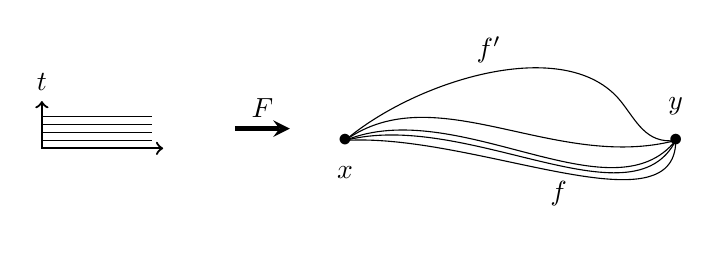
\begin{tikzpicture}[xscale=0.7, yscale=0.5]
		\draw [thick, <->] (1.5, 6.2) node [above] {$t$} -- (1.5, 5) -- (3.7, 5);
		\draw (1.5, 5.2) -- (3.5, 5.2);
		\draw (1.5, 5.4) -- (3.5, 5.4);
		\draw (1.5, 5.6) -- (3.5, 5.6);
		\draw (1.5, 5.8) -- (3.5, 5.8);

		\draw[-stealth, ultra thick] (5, 5.5) -- (6, 5.5) node[midway, above] {$F$};

		\coordinate (x) at (7, 5.2);
		\coordinate (y) at (13, 5.2);
		\node[label=below:$x$]  (x) at (7, 5.2) {$\bullet$};
		\node[label=above:$y$]  (y) at (13, 5.2) {$\bullet$};
		\draw (x.center) to [out=5, in=-90, edge node={node[below] {$f$}}] (y.center);
		\draw (x.center) to [out=20, in=-110] (y.center);
		\draw (x.center) to [out=30, in=-120] (y.center);
		\draw (x.center) to [out=45, in=-160] (y.center);
		\draw (x.center) to [out=50, in=-240, edge node={node[above] {$f'$}}]++(5, 1) to [out=-60, in=-170] (y.center);
	\end{tikzpicture}\end{center}
	Grupoid fundamental $\Pi_1(X)$ dari ruang $X$ didefinisikan sebagai kategori berikut. Objeknya adalah titik-titik dalam $X$, dan untuk setiap $x,y \in X$, himpunan morfisme $\Hom(x,y)$ didefinisikan sebagai himpunan semua kelas homotopi lintasan dari $x$ ke $y$. Komposisi morfisme didefinisikan melalui komposisi kelas lintasan, sedangkan morfisme identitas $\identity_x$ direpresentasikan oleh lintasan konstan $\forall t, \; \identity_x(t) = x$. Untuk morfisme tertentu $f: x \to y$ (yang dipandang sebagai suatu wakil dalam kelas homotopinya), inversnya dapat diambil sebagai lintasan berarah terbalik
	\[ f^{-1}(t) := f(1 - t), \quad 0 \leq t \leq 1. \]

	Dapat diperiksa bahwa semua operasi ini terdefinisi dengan baik dan menjadikan $\Pi_1(X)$ sebuah grupoid. Perhatikan bahwa $\Aut(x) = \Hom(x,x)$ tepat merupakan \emph{grup fundamental} $\pi_1(X, x)$ dengan titik dasar $x$.

	Grup fundamental merupakan invarian penting dalam topologi: kepada setiap ruang $X$ ia mengaitkan suatu struktur aljabar, yaitu grup. Grupoid fundamental dapat dipandang sebagai invarian satu tingkat lebih tinggi: kepada $X$ ia mengaitkan sebuah kategori. Untuk pembahasan lebih lanjut, lihat \cite[Bab 2]{May99}. Namun, pembaca perlu memperhatikan bahwa struktur kategoris $\Pi_1(X)$ masih mengabaikan banyak informasi topologis: selain kelas homotopi lintasan, seharusnya kita memperhitungkan semua homotopi di antara lintasan, kemudian homotopi di antara homotopi, dan seterusnya tanpa akhir. Semua ini harus dicerminkan dalam bahasa kategori yang lebih tinggi.
\end{example}

Akhirnya, kita perkenalkan sebuah konsep yang sederhana dan berguna: kategori lawan.
\begin{definition}\index{kategori!kategori lawan (opposite category)}\index[sym1]{Cop@$\mathcal{C}^\text{op}$}
	Untuk setiap kategori $\mathcal{C}$, \emph{kategori lawan} $\mathcal{C}^\text{op}$ didefinisikan sebagai berikut:
	\begin{compactitem}
		\item $\Obj(\mathcal{C}^{\text{op}}) = \Obj(\mathcal{C})$,
		\item untuk setiap objek $X,Y$, $\Hom_{\mathcal{C}^{\text{op}}}(X, Y) := \Hom_{\mathcal{C}}(Y, X)$,
		\item untuk morfisme $f \in \Hom_{\mathcal{C}^{\text{op}}}(Y, Z)$ dan $g \in \Hom_{\mathcal{C}^{\text{op}}}(X, Y)$, komposisi $f \circ^\text{op} g$ dalam $\mathcal{C}^{\text{op}}$ didefinisikan sebagai komposisi berurutan terbalik $g \circ f$ dalam $\mathcal{C}$,
		\item morfisme identitas didefinisikan sama seperti dalam $\mathcal{C}$.
	\end{compactitem}
\end{definition}
Mudah diperiksa bahwa $\mathcal{C}^\text{op}$ memenuhi definisi kategori dan bahwa $(\mathcal{C}^\text{op})^{\text{op}} = \mathcal{C}$. Singkatnya, konstruksi $\mathcal{C}^\text{op}$ membalikkan semua panah; setelah pembalikan, aksioma teori kategori tetap berlaku. Simetri dalam teori kategori ini disebut pula prinsip dualitas. Sebagai contoh, monomorfisme dalam $\mathcal{C}^\text{op}$ tidak lain adalah epimorfisme dalam $\mathcal{C}$. Dalam menangani banyak sifat kategoris, penggunaan simetri ini dengan tepat dapat sangat menyederhanakan pekerjaan.

\section{Fungtor dan Transformasi Natural}\label{sec:functors}
\begin{definition}[Fungtor]\label{def:functor}\index{fungtor@fungtor (functor)}
	Misalkan $\mathcal{C}', \mathcal{C}$ merupakan kategori. Sebuah fungtor $F: \mathcal{C}' \to \mathcal{C}$ terdiri atas data berikut:
	\begin{enumerate}[(i)]
		\item Peta antarobjek $F: \Obj(\mathcal{C}') \to \Obj(\mathcal{C})$.
		\item Peta antarmorfisme $F: \Mor(\mathcal{C}') \to \Mor(\mathcal{C})$, sedemikian sehingga
			\begin{compactitem}
				\item $F$ berkomutasi dengan peta sumber dan target (yakni $sF=Fs$, $tF=Ft$); secara ekuivalen, untuk setiap $X, Y \in \Obj(\mathcal{C}')$ terdapat peta $F: \Hom_{\mathcal{C}'}(X, Y) \to \Hom_{\mathcal{C}}(FX, FY)$;
				\item $F(g \circ f) = F(g) \circ F(f)$, $F(\identity_X) = \identity_{FX}$.
			\end{compactitem}
	\end{enumerate}
	Untuk $F: \mathcal{C}_1 \to \mathcal{C}_2$, $G: \mathcal{C}_2 \to \mathcal{C}_3$, fungtor komposit $G \circ F: \mathcal{C}_1 \to \mathcal{C}_3$ didefinisikan secara langsung dengan mengambil peta-peta komposit
	\begin{gather*}
		\Obj(\mathcal{C}_1) \xrightarrow{F} \Obj(\mathcal{C}_2) \xrightarrow{G} \Obj(\mathcal{C}_3), \\
		\Mor(\mathcal{C}_1) \xrightarrow{F} \Mor(\mathcal{C}_2) \xrightarrow{G} \Mor(\mathcal{C}_3).
	\end{gather*}
\end{definition}
Dalam literatur lama, fungtor di atas sering disebut fungtor kovarian dari $\mathcal{C}'$ ke $\mathcal{C}$, sedangkan fungtor berbentuk $F: (\mathcal{C}')^\text{op} \to \mathcal{C}$ disebut fungtor kontravarian.

\begin{remark}\label{rem:op-functor}
	Memberikan fungtor dari $\mathcal{C}'$ ke $\mathcal{C}$ sama saja dengan memberikan fungtor dari $(\mathcal{C}')^\text{op}$ ke $\mathcal{C}^\text{op}$. Untuk membedakannya, bagi fungtor $F: \mathcal{C}' \to \mathcal{C}$, fungtor yang bersesuaian di antara kategori lawan dinotasikan dengan $F^\text{op}: (\mathcal{C}')^\text{op} \to \mathcal{C}^\text{op}$.
\end{remark}

\begin{definition}\index{fungtor!penuh (full)}\index{fungtor!surjektif secara esensial (essentially surjective)}\index{fungtor!setia (faithful)}
	Untuk fungtor $F:  \mathcal{C}' \to \mathcal{C}$,
	\begin{enumerate}
		\item $F$ disebut surjektif secara esensial jika setiap objek dalam $\mathcal{C}$ isomorfik dengan suatu $FX$;
		\item $F$ disebut setia jika, untuk semua $X, Y \in \Obj(\mathcal{C}')$, peta $\Hom_{\mathcal{C}'}(X, Y) \to \Hom_{\mathcal{C}}(FX, FY) $ bersifat injektif;
		\item $F$ disebut penuh jika peta di atas bersifat surjektif untuk semua $X, Y \in \Obj(\mathcal{C}')$.
	\end{enumerate}
\end{definition}

\begin{example}\label{eg:functors}
	Fungtor yang digunakan dalam matematika amat banyak; berikut beberapa contoh singkat.
	\begin{enumerate}
		\item Subkategori $\mathcal{C}' \subset \mathcal{C}$ jelas memberikan fungtor inklusi $\iota: \mathcal{C}' \hookrightarrow \mathcal{C}$; fungtor inklusi selalu setia, dan ia penuh jika dan hanya jika $\mathcal{C}'$ merupakan subkategori penuh. Dengan mengambil $\mathcal{C}' = \mathcal{C}$, diperoleh fungtor identitas $\identity_{\mathcal{C}}: \mathcal{C} \to \mathcal{C}$.
		\item Perhatikan kategori grup $\cate{Grp}$. Untuk sebarang grup $G$, kita dapat melupakan struktur grup pada $G$ dan memandangnya sebagai himpunan; homomorfisme grup tentu dapat pula dipandang sebagai peta antarsimpunan. Prosedur ini memberikan \emph{fungtor pelupa} $\cate{Grp} \to \cate{Set}$. Fungtor pelupa untuk struktur lain didefinisikan dengan cara serupa, misalnya $\cate{Top} \to \cate{Set}$ (melupakan struktur topologis ruang), $\cate{Vect}(\Bbbk) \to \cate{Ab}$ (melupakan perkalian skalar pada ruang vektor-$\Bbbk$ $V$ dan hanya memandang grup aditifnya $(V, +)$, dengan $\Bbbk$ sebarang medan), dan sebagainya. Fungtor-fungtor seperti ini jelas setia, tetapi tidak penuh.\index{fungtor pelupa@fungtor pelupa (forgetful functor)}
		\item Perhatikan medan $\Bbbk$ beserta kategori ruang vektor di atasnya $\cate{Vect}(\Bbbk)$. Untuk sebarang ruang vektor-$\Bbbk$ $V$, definisikan ruang dualnya \index[sym1]{$V^\vee$}
			\[ V^\vee := \Hom_\Bbbk(V, \Bbbk) = \{ \Bbbk-\text{peta linear}\; V \to \Bbbk \}. \]
			Setiap peta linear $f: V_1 \to V_2$ menginduksi peta berarah sebaliknya pada ruang dual
			\begin{align*}
				f^\vee: V_2^\vee & \longrightarrow V_1^\vee, \\
				[\lambda: V_2 \to \Bbbk] & \longmapsto \lambda \circ f.
			\end{align*}
			Mudah dilihat bahwa $D: V \mapsto V^\vee$, $f \mapsto f^\vee$ mendefinisikan fungtor $D: \cate{Vect}(\Bbbk)^\text{op} \to \cate{Vect}(\Bbbk)$, dan dapat diperiksa bahwa $D$ setia. Menurut Catatan \ref{rem:op-functor}, kita memiliki fungtor komposit $D D^\text{op}: \cate{Vect}(\Bbbk) \to \cate{Vect}(\Bbbk)$.
			
			Dengan membatasi $D$ pada ruang vektor berdimensi hingga, diperoleh fungtor $D: \cate{Vect}_f(\Bbbk)^\text{op} \to \cate{Vect}_f(\Bbbk)$ dan $D D^\text{op}: \cate{Vect}_f(\Bbbk) \to \cate{Vect}_f(\Bbbk)$. Keduanya disebut, berturut-turut, fungtor dual dan fungtor dual ganda.
		\item Untuk sebarang grup $G$, definisikan subgrup turunan $G_\text{der}$ sebagai subgrup normal yang dibangkitkan oleh himpunan $\{xyx^{-1} y^{-1} : x,y \in G \}$. Grup hasil bagi $G/G_\text{der}$ merupakan grup abelian dan disebut abelianisasi dari $G$ (lihat Lema \ref{prop:abelianization}). Untuk sebarang homomorfisme grup $\varphi: G \to H$, dari definisi terlihat bahwa $\varphi(G_\text{der}) \subset H_\text{der}$; karena itu, $\varphi$ menginduksi homomorfisme grup abelian $\bar{\varphi}: G/G_\text{der} \to H/H_\text{der}$. Mudah diperiksa bahwa $G \mapsto G/G_\text{der}$, $\varphi \mapsto \bar{\varphi}$ mendefinisikan fungtor abelianisasi $\cate{Grp} \to \cate{Ab}$. Fungtor abelianisasi tidak setia.
		\item Kepada setiap ruang topologis bertitik dasar $(X,x)$, kaitkan grup fundamental $\pi_1(X, x)$; ini memberikan fungtor $\cate{Top}_\bullet \to \cate{Grp}$. Masih banyak contoh lain dalam topologi aljabar; misalnya, grup homologi suatu ruang $X \mapsto H_n(X; \Z)$ memberikan keluarga fungtor $H_n: \cate{Top} \to \cate{Ab}$, dengan $n \in \Z_{\geq 0}$, sedangkan grup kohomologi memberikan fungtor $H^n: \cate{Top}^\text{op} \to \cate{Ab}$.
	\end{enumerate}
\end{example}

\begin{definition}[Transformasi natural, atau morfisme antarfungtor]\index{transformasi natural@transformasi natural (natural transformation)}
	Di antara fungtor $F, G: \mathcal{C}' \to \mathcal{C}$, suatu transformasi natural $\theta$ adalah keluarga morfisme
	\[ \theta_X \in \Hom_{\mathcal{C}}(FX, GX), \quad X \in \Obj(\mathcal{C}'), \]
	sedemikian sehingga, dalam $\mathcal{C}'$, diagram berikut komutatif untuk setiap morfisme $f: X \to Y$
	\begin{equation}\label{eqn:naturaltrans-def}\begin{tikzcd}
		FX \arrow[r, "\theta_X"] \ar[d, "Ff"'] & GX \arrow[d, "Gf"] \\
		FY \arrow[r, "\theta_Y"'] & GY .
	\end{tikzcd}\end{equation}
	Transformasi natural di atas ditulis sebagai $\theta: F \to G$, atau digambarkan dengan diagram
	\[ \begin{tikzcd}
		\mathcal{C}' \arrow[bend left=50, r, "F", ""' name=U] \arrow[bend right=50, r, "G"', "" name=D] & \arrow[Rightarrow, to path=(U) -- (D) \tikztonodes, "\theta"] \mathcal{C}.
	\end{tikzcd} \]
\end{definition}
Diagram dengan panah ganda $\Rightarrow$ di atas kadang-kadang disebut pula sel-$2$; lihat \S\ref{sec:2-cat}. Sudut pandang yang barangkali lebih bermanfaat ialah membayangkan $\theta$ sebagai suatu homotopi dari $F$ ke $G$.

\begin{convention}\label{con:naturaltrans-morphism}\index{natural@natural}\index{kanonik@kanonik}
	Kita juga menyebut transformasi natural $\theta: F \to G$ sebagai morfisme dari fungtor $F$ ke $G$. Dalam penerapan, kerangka teori kategori yang ketat sering dihilangkan, dan cukup dikatakan bahwa morfisme $\theta_X: FX \to GX$ bersifat \emph{natural}, \emph{kanonik}, atau memenuhi \emph{fungtorialitas} terhadap peubah $X$. Dalam praktik, isomorfisme natural sering langsung ditulis sebagai tanda sama dengan $=$.
\end{convention}

Selanjutnya kita perkenalkan beberapa operasi pada transformasi natural, termasuk komposisi vertikal dan horizontal.\index{transformasi natural!komposisi}
\begin{itemize}
	\item Perhatikan tiga fungtor dari $\mathcal{C}'$ ke $\mathcal{C}$ beserta morfisme antarfungtor $\theta: F \to  G$,  $\psi: G \to H$. Komposisi vertikal $\psi \circ \theta$ didefinisikan sebagai $\{ \psi_X \circ \theta_X : X \in \Obj(\mathcal{C}') \}$, dan digambarkan sebagai berikut:
	\[\begin{tikzcd}
		\mathcal{C}'
			\arrow[bend left=70, rr, "F", ""' name=U]
			\arrow[rr, "G" name=MM, ""' name=M]
			\arrow[bend right=70, rr, "" name=D, "H"'] & &
		\arrow[Rightarrow, to path=(U) -- (MM) \tikztonodes, "\theta"] \arrow[Rightarrow, to path=(M) -- (D) \tikztonodes, "\psi"] \mathcal{C} 
	\end{tikzcd} \quad \text{dikomposisikan menjadi} \quad \begin{tikzcd}
		\mathcal{C}'
		\arrow[bend left=50, rr, "F", ""' name=U]
		\arrow[bend right=50, rr, "" name=D, "H"']
		& & \arrow[Rightarrow, to path=(U) -- (D) \tikztonodes, "\psi \circ \theta"] \mathcal{C} .
	\end{tikzcd}\]
	\item Perhatikan fungtor-fungtor
	$\begin{tikzcd}
		\mathcal{C}'' \arrow[bend left=30, r, "F_1"] \arrow[bend right=30, r, "F_2"] & \mathcal{C}' \arrow[bend left=30, r, "G_1"] \arrow[bend right=30, r, "G_2"] & \mathcal{C}
	\end{tikzcd}$
	dan morfisme $\theta: F_1 \to F_2$, $\psi: G_1 \to G_2$. Kita akan mendefinisikan komposisi horizontal $\psi \circ \theta: G_1 \circ F_1 \to G_2 \circ F_2$. Pertama, perhatikan bahwa bagi semua $X \in \Obj(\mathcal{C}'')$, dari naturalitas $\psi$, diagram
	\begin{equation}\label{eqn:horizontal-comp}\begin{tikzcd}
		G_1 F_1(X) \arrow[r, "{\psi_{F_1 X}}"] \arrow[d, "{G_1(\theta_X)}"'] & G_2 F_1(X) \arrow[d, "{G_2(\theta_X)}"] \\
		G_1 F_2(X) \arrow[r, "{\psi_{F_2 X}}"'] & G_2 F_2(X)
	\end{tikzcd}\end{equation}
	komutatif. Komposisi sepanjang diagonal $\searrow$ dinotasikan dengan $(\psi \circ \theta)_X : G_1 F_1 (X) \to G_2 F_2 (X)$; inilah komposisi horizontal yang dikehendaki. Kita akan segera membuktikan naturalitasnya, dan pembaca dapat memanfaatkan kesempatan ini untuk membiasakan diri menggunakan diagram komutatif. Diagramnya ialah:
	\[ \begin{tikzcd}
		\mathcal{C}'' \arrow[bend left=50, r, "F_1", ""' name=LU] \arrow[bend right=50, r, "" name=LD, "F_2"'] &
		\mathcal{C}' \arrow[bend left=50, r, "G_1", ""' name=RU] \arrow[bend right=50, r, "" name=RD, "G_2"'] &
		\arrow[Rightarrow, to path=(LU) -- (LD) \tikztonodes, "\theta"] \arrow[Rightarrow, to path=(RU) -- (RD) \tikztonodes, "\psi"] \mathcal{C}
	\end{tikzcd} \quad \text{dikomposisikan menjadi} \quad \begin{tikzcd}
		\mathcal{C}''
		\arrow[bend left=50, rr, "G_1 F_1", ""' name=U]
		\arrow[bend right=50, rr, "" name=D, "G_2 F_2"']
		& & \arrow[Rightarrow, to path=(U) -- (D) \tikztonodes, "\psi \circ \theta"] \mathcal{C} .
	\end{tikzcd} \]
	\item Komposisi horizontal mempunyai kasus khusus berikut. Perhatikan
	\[\begin{tikzcd}
		\mathcal{C}_1 \arrow[r, "H"] & \mathcal{C}_2 \arrow[bend left=50, r, "F", ""' name=U] \arrow[bend right=50, r, "" name=D, "G"'] & \mathcal{C}_3 \arrow[Rightarrow, to path=(U)--(D) \tikztonodes, "\theta"] \arrow[r, "K"] & \mathcal{C}_4 .
    \end{tikzcd} \]
	Pertama perhatikan tiga unsur di sebelah kiri: notasi $\theta H: FH \to GH$ kita gunakan sebagai singkatan bagi komposisi horizontal $\theta \circ \identity_{H}$; secara konkret, $(\theta H)_X = \theta_{HX} : FH(X) \to GH(X)$. Tiga unsur di sebelah kanan diperlakukan serupa: tuliskan $K\theta: KF \to KG$ untuk komposisi horizontal $\identity_K \circ \theta$, sehingga $(K\theta)_X = K(\theta_X): KF(X) \to KG(X)$.
\end{itemize}
Perhatikan bahwa kita menggunakan lambang yang sama $\circ$ untuk komposisi vertikal maupun horizontal; bila ada kemungkinan rancu, akan diberikan penjelasan tersendiri.

\begin{lemma}\label{prop:naturaltrans-associativity}
	Komposisi vertikal dan horizontal $\{ (\psi \circ \theta)_X \}_X$ yang didefinisikan di atas sama-sama merupakan morfisme antarfungtor, dan masing-masing memenuhi hukum asosiatif ketat $(\phi \circ \psi) \circ \theta = \phi \circ (\psi \circ \theta)$. Di antara komposisi vertikal dan horizontal berlaku hubungan berikut: untuk diagram
	\[\begin{tikzcd}
		\mathcal{C}_1
		\arrow[bend left=70, rr, ""' name=U]
		\arrow[rr, "" name=MM, ""' name=M]
		\arrow[bend right=70, rr, "" name=D] & &
		\arrow[Rightarrow, to path=(U) -- (MM) \tikztonodes, "\theta"] \arrow[Rightarrow, to path=  (M) -- (D) \tikztonodes, "\psi"] \mathcal{C}_2
		\arrow[bend left=70, rr, ""' name=V]
		\arrow[rr, "" name=NN, ""' name=N]
		\arrow[bend right=70, rr, "" name=E] & &
		\arrow[Rightarrow, to path=(V) -- (NN) \tikztonodes, "\theta'"] \arrow[Rightarrow, to path=  (N) -- (E) \tikztonodes, "\psi'"] \mathcal{C}_3 ,
	\end{tikzcd} \]
	berlaku hukum pertukaran berikut
	\[ \left( \psi' \underset{\text{vertikal}}{\circ} \theta'\right) \underset{\text{horizontal}}{\circ} \left( \psi \underset{\text{vertikal}}{\circ} \theta\right) = \left( \psi' \underset{\text{horizontal}}{\circ} \psi \right) \underset{\text{vertikal}}{\circ} \left( \theta' \underset{\text{horizontal}}{\circ} \theta\right).  \]
\end{lemma}
\begin{proof}
	Pernyataan mengenai komposisi vertikal mudah; berikut kita buktikan bahwa komposisi horizontal merupakan morfisme antarfungtor. Kita gunakan notasi sebelumnya. Dalam $\mathcal{C}''$, untuk morfisme $f: X \to Y$, perhatikan diagram yang berasal dari \eqref{eqn:horizontal-comp}
	\[\begin{tikzcd}
		G_1 F_1 (X) \arrow[r, "G_1 \theta_X"] \arrow[d, "G_1 F_1 f"'] & G_1 F_2 (X) \arrow[r, "{\psi_{F_2 X}}"] \arrow[d, "G_1 F_2 f"] & G_2 F_2 (X) \arrow[d, "G_2 F_2 f"] \\
		G_1 F_1 (Y) \arrow[r, "{G_1 \theta_Y}"'] & G_1 F_2 (Y) \arrow[r, "{\psi_{F_2 Y}}"'] & G_2 F_2 (Y) .
	\end{tikzcd} \]
	Menurut definisi, komposisi panah horizontal di baris atas dan bawah masing-masing adalah $(\psi \circ \theta)_X$ dan $(\psi \circ \theta)_Y$. Karena $\theta$ merupakan transformasi natural dan $G_1$ sebuah fungtor, persegi kiri komutatif; karena $\psi$ merupakan transformasi natural, persegi kanan pun komutatif. Dengan mengomposisikan panah-panah per bagian, diperoleh bahwa seluruh persegi besar komutatif; inilah sifat yang diperlukan bagi $ \psi \circ \theta$.

	Sekarang kita buktikan asosiativitas komposisi horizontal. Perhatikan morfisme-morfisme antarfungtor
	\[\begin{tikzcd}
		\mathcal{C}''' \arrow[bend left=50, r, "F_1", ""' name=LU] \arrow[bend right=50, r, "" name=LD, "F_2"'] &
		\mathcal{C}'' \arrow[bend left=50, r, "G_1", ""' name=MU] \arrow[bend right=50, r, "" name=MD, "G_2"'] &
		\mathcal{C}' \arrow[bend left=50, r, "H_1", ""' name=RU] \arrow[bend right=50, r, "" name=RD, "H_2"'] &
		\arrow[Rightarrow, to path=(LU) -- (LD) \tikztonodes, "\theta"]
		\arrow[Rightarrow, to path=(MU) -- (MD) \tikztonodes, "\psi"]
		\arrow[Rightarrow, to path=(RU) -- (RD) \tikztonodes, "\phi"]
		\mathcal{C} .
	\end{tikzcd} \]
	Untuk sebarang $X \in \Obj(\mathcal{C}''')$, perhatikan diagram
	\[\begin{tikzcd}[row sep=small]
		& & H_1 G_2 F_2(X) \arrow[rd] & \\
		H_1 G_1 F_1(X) \arrow[r] & H_1 G_2 F_1(X) \arrow[ru] \arrow[rd] & & H_2 G_2 F_2(X) . \\
		& & H_2 G_2 F_1(X) \arrow[ru] &
	\end{tikzcd}\]
	Dengan menerapkan naturalitas $\phi$ pada $G_2 F_1(X) \to G_2 F_2(X)$, bagian berbentuk belah ketupat diketahui komutatif. Komposisi sepanjang lintasan
	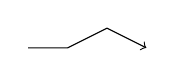
\begin{tikzpicture}[scale=0.5, baseline=(X)]
		\draw[->] (0,0) -- (1,0) -- (2, 0.5) -- (3, 0);
		\coordinate (X) at (0,0);
	\end{tikzpicture}
	menghasilkan $(\phi \circ (\psi \circ \theta))_X$. Sementara itu, komposisi sepanjang lintasan
	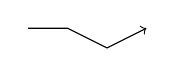
\begin{tikzpicture}[scale=0.5, baseline=(X)]
		\draw[->] (0,0) -- (1,0) -- (2, -0.5) -- (3, 0);
		\coordinate (X) at (0, -0.2);
	\end{tikzpicture}
	menghasilkan $((\phi \circ \psi) \circ \theta)_X$; di sini kita masih perlu menggunakan diagram komutatif \eqref{eqn:horizontal-comp}. Asosiativitas pun terbukti.

	Persamaan terakhir dapat diperoleh secara serupa dengan menelusuri diagram; rinciannya diserahkan kepada pembaca yang berminat.
\end{proof}

Setiap fungtor $F$ mempunyai morfisme identitas ke dirinya sendiri, $\identity_F : F \to F$. Diberikan morfisme antarfungtor $\theta: F_1 \to F_2$, jika morfisme $\psi: F_2 \to F_1$ memenuhi $\psi \circ \theta = \identity_{F_1}$, $\theta \circ \psi = \identity_{F_2}$, maka $\psi$ disebut invers dari $\theta$. Morfisme invertibel disebut isomorfisme antarfungtor dan ditulis $\theta: F_1 \rightiso F_2$. Langsung dari definisi terlihat bahwa invers $\theta$, jika ada, bersifat tunggal dan dinotasikan dengan $\theta^{-1}$; invers ini tidak lain diperoleh dengan mengambil invers ``titik demi titik'' dalam kategori: $(\theta^{-1})_X := (\theta_X)^{-1}: F_2 X \rightiso F_1 X$. Demikian pula, morfisme $\theta$ invertibel jika dan hanya jika setiap $\theta_X$ invertibel. Mudah dilihat bahwa komposisi vertikal maupun horizontal dari isomorfisme tetap merupakan isomorfisme. Pernyataan ekuivalen bagi isomorfisme antarfungtor $\theta: F_1 \rightiso F_2$ ialah bahwa $\theta_X: F_1 X \rightiso F_2 X$ merupakan \emph{isomorfisme natural} atau \emph{isomorfisme kanonik} terhadap peubah $X$.

\begin{definition}[Ekuivalensi]\label{def:cat-equivalence}\index{ekuivalensi kategori@ekuivalensi kategori (equivalence)}\index{fungtor!kuasi-invers (quasi-inverse)}
	Jika sepasang fungtor
	\begin{tikzcd}
		\mathcal{C}_1 \arrow[bend left=20, r, "F"] & \mathcal{C}_2 \arrow[bend left=20, l, "G"]
	\end{tikzcd}
	memenuhi sifat berikut: terdapat isomorfisme antarfungtor $\theta: FG \rightiso \identity_{\mathcal{C}_2}$, $\psi: GF \rightiso \identity_{\mathcal{C}_1}$, maka $G$ disebut, bagi $F$, \emph{fungtor kuasi-invers}, dan $F$ disebut ekuivalensi dari kategori $\mathcal{C}_1$ ke $\mathcal{C}_2$, atau singkatnya suatu \emph{ekuivalensi}.

	Jika lebih lanjut $FG = \identity_{\mathcal{C}_2}$, $GF = \identity_{\mathcal{C}_1}$, maka $F$ disebut \emph{isomorfisme} antarkategori, sedangkan $G$ disebut \emph{invers} dari $F$.
\end{definition}
Mudah dibuktikan bahwa komposisi ekuivalensi tetap merupakan ekuivalensi; rinciannya dijadikan latihan.

\begin{example}
	Misalkan $\cate{CHaus}$ adalah kategori ruang topologis kompak Hausdorff, dan $C^*\dcate{CommAlg}$ kategori aljabar-$C^*$ komutatif berunsur satuan (dengan morfisme berupa homomorfisme-$\ast$ yang mempertahankan unsur satuan). Versi komutatif teorema Gelfand--Naimark menyatakan bahwa fungtor-fungtor
	\[ \begin{tikzcd}[row sep=tiny]
		\cate{CHaus}^{\text{op}} \arrow[yshift=0.7ex]{r} & C^*\dcate{CommAlg} \arrow[yshift=-0.7ex]{l} \\
		X \arrow[mapsto]{r} & C(X): \text{ruang fungsi kontinu bernilai kompleks} \\
		\mathfrak{M}_A: \text{ ruang ideal maksimal} & A \arrow[mapsto]{l}
	\end{tikzcd} \]
	saling kuasi-invers: transformasi Gelfand $a \mapsto \hat{a}$ memberikan isomorfisme natural $A \rightiso C(\mathfrak{M}_A)$; lihat \cite[Teorema 5.4.8]{Zh2}. Isomorfisme natural pada arah sebaliknya, $X \rightiso \mathfrak{M}_{C(X)}$, relatif lebih mudah; lihat \cite[Teorema 5.3.2]{Zh2}.
\end{example}

\begin{proposition}
	Jika $G, G'$ merupakan kuasi-invers dari fungtor $F: \mathcal{C}_1 \to \mathcal{C}_2$, maka terdapat isomorfisme antarfungtor $G \simeq G'$.
\end{proposition}
\begin{proof}
	Komposisi horizontal transformasi natural memberikan $G \xleftarrow[\sim]{\psi' \circ \identity_G} (G'F)G = G'(FG) \xrightarrow[\sim]{\identity_{G'} \circ \theta} G'$.
\end{proof}

\begin{remark}\label{rem:strict-or-not}
	Kita telah mendefinisikan konsep invers bagi morfisme antarobjek dan morfisme antarfungtor (transformasi natural); invers tersebut, jika ada, bersifat tunggal, dan dari sinilah isomorfisme antarobjek atau antarfungtor didefinisikan. Konsep invers dapat pula didefinisikan bagi fungtor, dan fungtor invers, jika ada, bersifat tunggal. Sebaliknya, dua fungtor kuasi-invers dapat berbeda hingga suatu isomorfisme. Praktik menunjukkan bahwa konsep isomorfisme kategori kurang berguna, sedangkan konsep ekuivalensi muncul di mana-mana. Hal ini mencerminkan suatu kaidah praktis dalam teori kategori: pada tingkat fungtor, isomorfisme (seperti $\theta: FG \rightiso \identity$ di atas) hampir selalu lebih berguna daripada kesamaan ketat (seperti $FG = \identity$ di atas). Namun, isomorfisme itu pun tidak boleh sebarang; syarat yang diperlukan biasanya disebut koherensi. Dalam kasus ekuivalensi, pembaca mungkin telah merasakan dalam argumen sebelumnya bahwa konsep kuasi-invers agak longgar; Teorema \ref{prop:adjoint-equivalence} akan memberikan suatu penyempurnaan yang disebut \emph{ekuivalensi adjoin}. \index{ekuivalensi adjoin@ekuivalensi adjoin (adjoint equivalence)}
\end{remark}

Subkategori penuh $\mathcal{C}' \subset \mathcal{C}$ disebut, bagi $\mathcal{C}$, suatu \emph{kerangka} jika setiap objek dalam $\mathcal{C}$, katakan $X$, memiliki isomorfisme $X \rightiso Y \in \Obj(\mathcal{C}')$, dan $Y \in \Obj(\mathcal{C}')$ tersebut tunggal. Kategori yang merupakan kerangka bagi dirinya sendiri disebut \emph{kategori skeletal}.\index{kategori!kerangka (skeleton)}

\begin{lemma}\label{prop:skeletal-cat-isom}
	Setiap kategori $\mathcal{C}$ memiliki suatu kerangka $\mathcal{C}'$, dan fungtor inklusi $\iota: \mathcal{C}' \hookrightarrow \mathcal{C}$ merupakan ekuivalensi. Setiap fungtor penuh, setia, dan surjektif secara esensial di antara kategori skeletal merupakan isomorfisme.
\end{lemma}
\begin{proof}
	Kita buktikan dahulu bagian pertama. Dengan aksioma pilihan, pilih satu wakil dari setiap kelas isomorfisme dalam $\Obj(\mathcal{C})$, lalu nyatakan subkategori penuh yang dibentuk oleh wakil-wakil tersebut sebagai $\mathcal{C}'$. Demikian pula, untuk setiap $X \in \Obj(\mathcal{C})$, kita dapat memilih isomorfisme $\theta_X: X \rightiso \kappa(X) $, dengan $\kappa(X) \in \Obj(\mathcal{C}')$; tanpa mengurangi keumuman, andaikan bagi $X \in \Obj(\mathcal{C}')$ berlaku $\theta_X = \identity_X$. Ada tepat satu cara memperluas $\kappa: \Obj(\mathcal{C}) \to \Obj(\mathcal{C}')$ menjadi fungtor sedemikian sehingga $\theta: \identity_{\mathcal{C}} \rightiso \iota \kappa$: tetapkan
	\[ \kappa(f) := \theta_Y \circ f \circ \theta_X^{-1} \in \Hom_{\mathcal{C}'}(\kappa(X), \kappa(Y)), \quad f \in \Hom_{\mathcal{C}}(X, Y). \]
	Di sisi lain, kita memiliki kesamaan fungtor $\kappa\iota = \identity_{\mathcal{C}'}$. Jadi, $\kappa$ merupakan fungtor kuasi-invers dari $\iota$.
	
	Untuk bagian kedua, misalkan $F: \mathcal{C}_1 \to \mathcal{C}_2$ adalah fungtor penuh, setia, dan surjektif secara esensial di antara kategori skeletal. Untuk sebarang objek dalam $\mathcal{C}_2$, katakan $Z$, terdapat $X$ sedemikian sehingga $Z \simeq FX$, dan karena itu $Z = FX$. Objek $X$ seperti ini tunggal, sebab sifat penuh dan setia bersama $FX \simeq FX'$ mengakibatkan $X \simeq X'$. Dengan demikian, $F$ bijektif pada himpunan objek, sehingga fungtor inversnya $G$ dapat didefinisikan.
\end{proof}

\begin{theorem}\label{prop:functor-equiv-criterion}\index{ekuivalensi kategori@ekuivalensi kategori (equivalence)}
	Untuk fungtor $F: \mathcal{C}_1 \to \mathcal{C}_2$, pernyataan-pernyataan berikut ekuivalen.
	\begin{compactenum}
		\item $F$ merupakan ekuivalensi kategori,
		\item $F$ merupakan fungtor penuh, setia, dan surjektif secara esensial.
	\end{compactenum}
\end{theorem}
\begin{proof}
	Andaikan $F$ merupakan ekuivalensi kategori. Ambil fungtor kuasi-invers $G: \mathcal{C}_2 \to \mathcal{C}_1$ beserta $GF \xrightarrow[\sim]{\psi} \identity_{\mathcal{C}_1}$, $FG \xrightarrow[\sim]{\phi} \identity_{\mathcal{C}_2}$. Untuk setiap objek dalam $\mathcal{C}_2$, katakan $Z$, terdapat $\phi_Z: F(GZ) \rightiso Z$, sehingga $F$ surjektif secara esensial; dengan cara yang sama, $G$ juga surjektif secara esensial. Perhatikan bahwa
	\[\begin{tikzcd}[row sep=tiny, column sep=small]
		\Hom(X,Y) \arrow[r, "F"] & \Hom(FX, FY) \arrow[r, "G"] & \Hom(GF(X), GF(Y)) \arrow[r, "\sim"] & \Hom(X, Y) \\
		f \arrow[mapsto, r] & Ff \arrow[mapsto, r] & GF(f) \arrow[mapsto, r] & \psi_Y GF(f) \psi_X^{-1}
	\end{tikzcd}\]
	komposisinya merupakan peta identitas; jadi, panah pertama $F$ pada diagram mempunyai invers kiri, sedangkan panah kedua $G$ mempunyai invers kanan. Dengan menukar peran $F, G$, terlihat bahwa apabila $X, Y \in \Obj(\mathcal{C}_1)$ termasuk dalam citra $G$, peta $\Hom(X, Y) \xrightarrow{F} \Hom(FX, FY)$ mempunyai invers kanan. Akan tetapi, setiap objek dalam $\mathcal{C}_1$ isomorfik dengan suatu objek dalam citra $G$; karena itu, $F$ merupakan fungtor penuh dan setia.

	Sekarang kita buktikan arah sebaliknya. Dengan Lema \ref{prop:skeletal-cat-isom}, ambil kerangka $\iota_i: \mathcal{C}'_i \rightarrow \mathcal{C}_i$ beserta fungtor kuasi-inversnya $\kappa_i$ (di sini $i=1,2$). Fungtor $F' := \kappa_2 \circ F \circ \iota_1: \mathcal{C}'_1 \to \mathcal{C}'_2$ tetap penuh, setia, dan surjektif secara esensial; jadi, $F'$ merupakan isomorfisme kategori. Tetapkan $G := \iota_1 \circ F'^{-1} \circ \kappa_2$; maka
	\begin{gather*}
		GF = \iota_1  F'^{-1} \kappa_2 F \simeq \iota_1  F'^{-1} \underbracket{\kappa_2 F \iota_1}_{= F'} \kappa_1 = \iota_1 \kappa_1 \simeq \identity_{\mathcal{C}_1}, \\
		FG = F \iota_1  F'^{-1} \kappa_2 \simeq \iota_2 \underbracket{\kappa_2 F \iota_1}_{= F'}  F'^{-1} \kappa_2 = \iota_2 \kappa_2 \simeq \identity_{\mathcal{C}_2}.
	\end{gather*}
	Di sini kita telah menggunakan komposisi horizontal transformasi natural.
\end{proof}

\begin{example}\label{eg:vectf-duality}
	Masih dengan medan $\Bbbk$, perhatikan kembali kategori ruang vektor di atasnya $\cate{Vect}(\Bbbk)$ beserta subkategorinya $\cate{Vect}_f(\Bbbk)$. Dalam Contoh \ref{eg:functors}, telah didefinisikan fungtor dual ganda $D D^\text{op}: \cate{Vect}(\Bbbk) \to \cate{Vect}(\Bbbk)$. Untuk setiap ruang vektor $V$, terdapat peta evaluasi
	\begin{align*}
		\text{ev}: V & \longrightarrow DD^\text{op} V = (V^\vee)^\vee \\
		v & \longmapsto [\lambda \mapsto \lambda(v)].
	\end{align*}
	Untuk sebarang peta linear $f: V \to W$, dari definisi $f^\vee$ tidak sulit diperiksa bahwa diagram berikut
	\[\begin{tikzcd}
		V \arrow[r, "\text{ev}"] \ar[d, "f"'] & DD^\text{op} V \arrow[d, "{DD^\text{op} f}"] \\
		W \ar[r, "\text{ev}"'] & DD^\text{op} W
	\end{tikzcd} \]
	komutatif, sehingga diperoleh $\text{ev}: \identity \to D D^\text{op}$. Mudah dilihat bahwa $\text{ev}: V \to D D^\text{op} V$ selalu injektif; bahkan dapat dibuktikan bahwa $\text{ev}$ bijektif jika dan hanya jika $V$ berdimensi hingga. Setelah semuanya dibatasi pada subkategori penuh $\cate{Vect}_f(\Bbbk)$, diperoleh isomorfisme
	\[ \text{ev}: \identity_{\cate{Vect}_f(\Bbbk)} \rightiso D D^\text{op}. \]
	Jika rumus yang sama ditafsirkan dalam kategori lawan, diperoleh
	\[ \identity_{\cate{Vect}_f(\Bbbk)^\text{op}} \rightiso D^\text{op} D. \]
	Jadi, fungtor $D: \cate{Vect}_f(\Bbbk)^\text{op} \to \cate{Vect}_f(\Bbbk)$ merupakan ekuivalensi antarkategori, sedangkan $D^\text{op}: \cate{Vect}_f(\Bbbk) \to \cate{Vect}_f(\Bbbk)^\text{op}$ merupakan kuasi-inversnya.
\end{example}

\begin{example}
	Pilih sebuah medan $\Bbbk$, dan definisikan kategori $\cate{Mat}$ sebagai berikut: objek-objeknya adalah $\Z_{\geq 0}$; untuk sebarang objek $n, m \in \Z_{\geq 0}$, definisikan $\Hom(n, m) := M_{m \times n}(\Bbbk)$ sebagai himpunan semua matriks di atas medan $\Bbbk$ yang berukuran $m \times n$, yaitu $A = (a_{ij})_{\substack{1 \leq i \leq m \\ 1 \leq j \leq n}}$. Dengan konvensi $M_{0 \times n}(\Bbbk) = M_{m \times 0}(\Bbbk) := \{0\}$, komposisi morfisme didefinisikan sebagai perkalian matriks biasa
	\begin{align*}
		\Hom(n, m) \times \Hom(m, k) & \longrightarrow \Hom(n, k) \\
		(A, B) & \longmapsto BA .
	\end{align*}

	Definisikan fungtor $F: \cate{Mat} \to \cate{Vect}_f(\Bbbk)$ sebagai berikut: tetapkan $F(n) = \Bbbk^{\oplus n} := M_{n \times 1}(\Bbbk)$; untuk $A \in \Hom(n, m)$, peta linear $FA: \Bbbk^{\oplus n} \to \Bbbk^{\oplus m}$ adalah perkalian matriks $v \mapsto Av$. Kita menyatakan bahwa $F$ merupakan ekuivalensi kategori.

	Semua ini hanyalah aljabar linear yang tampak lebih megah daripada sebenarnya. Pertama, perhatikan bahwa $F: \Hom(n, m) \to \Hom_\Bbbk(\Bbbk^{\oplus n}, \Bbbk^{\oplus m})$ merupakan bijeksi; ini tidak lain adalah representasi matriks suatu peta linear. Selanjutnya, dari $V \simeq \Bbbk^{\oplus \dim V}$ (dengan $V$ ruang vektor-$\Bbbk$) diketahui bahwa $F$ penuh, setia, dan surjektif secara esensial; menurut Teorema \ref{prop:functor-equiv-criterion}, fungtor tersebut merupakan ekuivalensi kategori.
\end{example}

\section{Kategori Fungtor}\label{sec:functor-category}
Pertama-tama kita definisikan konsep produk dan koproduk (juga disebut gabungan saling lepas) kategori; konsep-konsep ini sangat berguna untuk menyatakan sejumlah sifat kategori.

Ingat kembali Konvensi \ref{con:U-small}: kecuali dinyatakan lain, kategori yang dibahas berikut ini semuanya merupakan kategori-$\mathcal{U}$, dengan $\mathcal{U}$ semesta yang telah dipilih. Himpunan yang termasuk dalam $\mathcal{U}$ disebut himpunan-$\mathcal{U}$.

\begin{definition}\index{kategori!produk, koproduk}
	Misalkan $I$ merupakan himpunan-$\mathcal{U}$ dan $\{\mathcal{C}_i : i \in I \}$ suatu keluarga kategori.
	\begin{itemize}
		\item Kategori produk $\prod_{i \in I} \mathcal{C}_i$ didefinisikan sebagai berikut:
			\begin{align*}
				\Obj\left( \prod_{i \in I} \mathcal{C}_i \right) & := \prod_{i \in I} \Obj(\mathcal{C}_i), \\
				\Hom_{\prod_{i \in I} \mathcal{C}_i}( (X_i)_i, (Y_i)_i ) & := \prod_{i \in I} \Hom_{\mathcal{C}_i}(X_i, Y_i),
			\end{align*}
			dengan $(X_i)_i$ menyatakan suatu unsur dari $\prod_{i \in I} \Obj(\mathcal{C}_i)$. Komposisi morfisme didefinisikan per komponen.
		\item Kategori koproduk (juga disebut gabungan saling lepas) $\coprod_{i \in I} \mathcal{C}_i$ didefinisikan sebagai berikut:
			\begin{align*}
				\Obj\left( \coprod_{i \in I} \mathcal{C}_i \right) & := \coprod_{i \in I} \Obj(\mathcal{C}_i), \\
				\Hom_{\coprod_{i \in I} \mathcal{C}_i}(X_j, X'_k) & :=
				\begin{cases}
					\Hom_{\mathcal{C}_j}(X_j, X'_k), & j = k, \\
					\emptyset, & j \neq k;
				\end{cases}
			\end{align*}
			di sini, untuk setiap $j \in I$, berlaku $X_j, X'_j \in \Obj(\mathcal{C}_j)$. Komposisi morfisme didefinisikan secara terpisah di dalam setiap $\mathcal{C}_i$.
	\end{itemize}
\end{definition}
Karena $I$ diasumsikan sebagai himpunan-$\mathcal{U}$, kategori yang dikonstruksi di atas tetap merupakan kategori-$\mathcal{U}$; jika setiap $\mathcal{C}_i$ merupakan kategori kecil-$\mathcal{U}$, maka produk dan koproduknya pun demikian.

Kita memiliki keluarga fungtor proyeksi $\pr_j: \prod_{i \in I} \mathcal{C}_i \to \mathcal{C}_j$, yang memetakan $(X_i)_i$ ke $X_j$ dan, pada tingkat morfisme, secara serupa memproyeksikan ke komponen ke-$j$. Demikian pula, didefinisikan keluarga fungtor inklusi $\iota_j: \mathcal{C}_j \to \coprod_{i \in I} \mathcal{C}_i$, yang menyisipkan $\mathcal{C}_j$ dengan cara yang jelas sebagai subkategori penuh.

Khususnya, dengan mengambil $I$ sebagai himpunan hingga, kita dapat mendefinisikan $\mathcal{C}_1 \times \cdots \times \mathcal{C}_n$ dan $\mathcal{C}_1 \sqcup \cdots \sqcup \mathcal{C}_n$.

\begin{definition}
	Fungtor berbentuk $F: \mathcal{C}_1 \times \mathcal{C}_2 \to \mathcal{C}$ disebut fungtor biner. Fungtor banyak peubah $\mathcal{C}_1 \times \cdots \times \mathcal{C}_n \to \mathcal{C}$ didefinisikan secara serupa.
\end{definition}

\begin{example}[Fungtor $\Hom$]\label{eg:Hom-functor} \index[sym1]{HomC}
	Untuk kategori $\mathcal{C}$, pemetaan $(X,Y)\mapsto\Hom_{\mathcal{C}}(X,Y)$ mendefinisikan fungtor biner
	\[ \Hom_{\mathcal{C}}: \mathcal{C}^\text{op} \times \mathcal{C}  \to \cate{Set}. \]
	Memang, setiap pasangan morfisme $f: X' \to X$, $g: Y \to Y'$ dalam $\mathcal{C}$ menginduksi
	\begin{align*}
		\Hom_{\mathcal{C}}(X, Y) & \longrightarrow \Hom_{\mathcal{C}}(X', Y') \\
		\phi & \longmapsto g \phi f .
	\end{align*}
	Kadang-kadang hal ini juga dikatakan sebagai \emph{tarik balik} morfisme $\phi$ sepanjang $f$ dan \emph{dorong maju} sepanjang $g$. Tarik balik dan dorong maju lazim dinotasikan dengan $f^* \phi = \phi f$ dan $g_* \phi = g\phi$.\index{tarik balik@tarik balik (pullback)}\index{dorong maju@dorong maju (pushforward)}\index[sym1]{$f_*, f^*$}
	Mudah dilihat bahwa $(f_1 f_2)^* = f_2^* f_1^*$ dan $(f_1 f_2)_* = (f_1)_* (f_2)_*$.
\end{example}

\begin{definition}[Kategori fungtor]\index{kategori fungtor@kategori fungtor (functor category)}\index[sym1]{Fct@$\text{Fct}$}
	Misalkan $\mathcal{C}_1, \mathcal{C}_2$ merupakan kategori-$\mathcal{U}$. Definisikan kategori fungtor $\text{Fct}(\mathcal{C}_1, \mathcal{C}_2)$ sebagai berikut: objeknya adalah fungtor dari $\mathcal{C}_1$ ke $\mathcal{C}_2$, dan morfisme di antara sebarang dua objek $F, G$ adalah transformasi natural $\theta: F \to G$; komposisi morfisme $\theta: F \to G$ dan $\psi: G \to H$ adalah komposisi vertikal transformasi natural $\psi \circ \theta: F \to H$.
\end{definition}
Konstruksi ini menjelaskan Konvensi \ref{con:naturaltrans-morphism}.

\begin{remark}
	Definisi ini memerlukan sedikit penjelasan. Pertama, perhatikan bahwa objek dan morfisme $\text{Fct}(\mathcal{C}_1, \mathcal{C}_2)$ masing-masing membentuk himpunan. Untuk morfisme terdapat hasil yang lebih tepat: jika $\mathcal{C}_1$ merupakan kategori kecil-$\mathcal{U}$, maka $\text{Fct}(\mathcal{C}_1, \mathcal{C}_2)$ merupakan kategori-$\mathcal{U}$, sebab bagi sebarang dua fungtor $F, G: \mathcal{C}_1 \to \mathcal{C}_2$, transformasi natural di antaranya membentuk subhimpunan dari himpunan
	\[ \prod_{X \in \Obj(\mathcal{C}_1)} \Hom_{\mathcal{C}_2} (FX, GX) \]
	Jika $\mathcal{C}_1$ merupakan kategori kecil-$\mathcal{U}$, maka himpunan di atas merupakan himpunan kecil-$\mathcal{U}$.

	Selain itu, diperlukan pula asosiativitas komposisi vertikal transformasi natural; lihat Lema \ref{prop:naturaltrans-associativity}.
\end{remark}

Bagi fungtor $F, G : \mathcal{C}_1 \to \mathcal{C}_2$, pada kategori lawan terdapat fungtor yang bersesuaian $F^\text{op}, G^\text{op}: \mathcal{C}_1^\text{op} \to \mathcal{C}_2^\text{op}$ (lihat Catatan \ref{rem:op-functor}). Mudah dilihat bahwa transformasi natural $\varphi: F \to G$ dibalik pada kategori lawan menjadi $\varphi^\text{op}: G^\text{op} \to F^\text{op}$, dan bahwa $(\varphi^{\text{op}})^{\text{op}} = \varphi$. Hal ini dirangkum sebagai berikut.

\begin{proposition}\label{prop:op-functor-cat}
	Terdapat isomorfisme natural $\text{Fct}(\mathcal{C}_1, \mathcal{C}_2)^\text{op} \rightiso \text{Fct}(\mathcal{C}_1^{\text{op}}, \mathcal{C}_2^{\text{op}})$ yang memetakan $\varphi$ ke $\varphi^\text{op}$.
\end{proposition}

Dalam kebanyakan penggunaan selanjutnya, $\mathcal{C}_1$ merupakan kategori kecil. Kadang-kadang $\text{Fct}(\mathcal{C}_1, \mathcal{C}_2)$ juga ditulis sebagai $\mathcal{C}_2^{\mathcal{C}_1}$.
\begin{example}
	Perhatikan himpunan $I \in \mathcal{U}$ dan ambil $\mathcal{I} := \cate{Disc}(I)$ sebagai kategori diskret yang bersesuaian (Contoh \ref{eg:categories}). Maka, untuk setiap $\mathcal{C}$, terdapat isomorfisme kategori $\mathcal{C}^{\mathcal{I}} \simeq \prod_{i \in I} \mathcal{C}$.
\end{example}

Setelah kategori fungtor didefinisikan, di dalamnya kita tentu dapat membahas monoid endomorfisme $\End(F)$ dan grup automorfisme $\Aut(F)$ dari suatu fungtor $F: \mathcal{C}_1 \to \mathcal{C}_2$. Sebagai himpunan, keduanya belum tentu termasuk dalam $\mathcal{U}$.
\begin{definition}\label{def:cat-center}\index{pusat kategori@pusat kategori (center)}
	\emph{Pusat} suatu kategori $\mathcal{C}$ didefinisikan sebagai $Z(\mathcal{C}) := \End(\identity_{\mathcal{C}})$.
\end{definition}

Pusat merupakan suatu invarian kategori yang sangat berguna. Menurut \eqref{eqn:naturaltrans-def}, unsur $Z(\mathcal{C})$ tidak lain adalah keluarga endomorfisme $\psi_X: X \to X$ sedemikian sehingga diagram
\begin{tikzcd}
	X \arrow[r, "{\psi_X}"] \arrow[d, "f"'] & X \arrow[d, "f"] \\
	Y \arrow[r, "{\psi_Y}"'] & Y
\end{tikzcd}
komutatif untuk setiap $f: X \to Y$.

\begin{proposition}
	Pusat $Z(\mathcal{C})$ selalu komutatif terhadap operasi biner $\circ$.
\end{proposition}
\begin{proof}
	Diberikan $\theta, \psi \in \End(\identity_{\mathcal{C}})$, ambil endomorfisme $\theta$, objek $X=Y$, dan morfisme $f = \psi_X$ pada diagram di atas; diperoleh $\theta_X \psi_X = \psi_X \theta_X$.
\end{proof}

\begin{proposition}
	Ekuivalensi kategori $F: \mathcal{C}_1 \to \mathcal{C}_2$ menginduksi isomorfisme pusat $Z(\mathcal{C}_1) \simeq Z(\mathcal{C}_2)$.
\end{proposition}
Pembuktiannya mudah dan diserahkan sebagai latihan.

\section{Sifat Universal}\label{sec:cat-universals}
Banyak konstruksi matematika dapat dicirikan secara unik oleh sifat universal. Kita menguraikannya dengan bahasa objek awal, objek terminal, dan kategori koma.

\begin{definition}\label{def:universal-objects}\index{objek!objek awal/objek terminal/objek nol (initial/terminal/zero object)}
	Dalam kategori $\mathcal{C}$, objek $X$ disebut \emph{objek awal} jika, untuk setiap objek $Y$, himpunan $\Hom_{\mathcal{C}}(X, Y)$ memiliki tepat satu unsur. Demikian pula, $X$ disebut \emph{objek terminal} jika, untuk setiap objek $Y$, himpunan $\Hom_{\mathcal{C}}(Y, X)$ memiliki tepat satu unsur. Jika $X$ merupakan objek awal sekaligus objek terminal, maka disebut \emph{objek nol}.
\end{definition}

Objek awal dan objek terminal merupakan konsep yang saling dual: objek awal dari $\mathcal{C}$ tidak lain adalah objek terminal dari $\mathcal{C}^\text{op}$, dan sebaliknya.

\begin{proposition}\label{prop:initial-obj-uniqueness}
	Misalkan $X, X'$ merupakan objek awal dalam $\mathcal{C}$. Maka terdapat tepat satu isomorfisme $X \rightiso X'$. Pernyataan serupa berlaku untuk objek terminal.
\end{proposition}
\begin{proof}
	Cukup tangani kasus objek awal. Misalkan $X, X'$ keduanya merupakan objek awal. Maka terdapat tepat satu morfisme $f: X \to X'$ dan $g: X' \to X$. Komposisinya $gf: X \to X$ juga tunggal, sehingga harus sama dengan $\identity_X$; dengan cara yang sama, $fg = \identity_{X'}$. Jadi, $f: X \rightiso X'$ adalah isomorfisme yang dicari.
\end{proof}

\begin{definition}\label{def:zero-morphism}\index{morfisme!morfisme nol (zero morphism)}
	Misalkan $\mathcal{C}$ memiliki objek nol, yang kita nyatakan dengan $0$. Untuk sebarang $X, Y \in \Obj(\mathcal{C})$, definisikan \emph{morfisme nol} $0: X \to Y$ sebagai
	\[ X \to 0 \to Y \]
	komposisi kedua morfisme tersebut.
\end{definition}

Dua pengamatan: (1) Komposisi morfisme nol dari kiri maupun dari kanan dengan sebarang morfisme tetap merupakan morfisme nol. (2) Definisi morfisme nol tidak bergantung pada pilihan objek nol: jika $0, 0'$ keduanya merupakan objek nol, setiap panah yang masuk ke atau keluar dari $0, 0'$ ditentukan secara unik, sehingga diagram di bawah komutatif secara otomatis.
\[ \begin{tikzcd}[row sep=small]
	{} & 0 \arrow[rd] \arrow[dd, "\simeq"] & {} \\
	X \arrow[ru] \arrow[rd] & & Y . \\
	& 0' \arrow[ru] &
\end{tikzcd} \]

\begin{example}
	Secara umum, objek awal dan objek terminal tidak selalu ada (contoh: kategori diskret). Berikut beberapa contoh yang khas:
	\begin{enumerate}
		\item Kategori himpunan $\cate{Set}$: $\emptyset$ merupakan objek awal, sedangkan $\{\text{pt}\}$ merupakan objek terminal;
		\item Kategori himpunan bertitik $\cate{Set}_\bullet$: $(\{\text{pt}\}, \text{pt})$ merupakan objek nol;
		\item Kategori grup $\cate{Grp}$: grup trivial $\{1\}$ merupakan objek nol, dan homomorfisme konstan bernilai $1$ merupakan morfisme nol;
		\item Kategori ruang vektor atas medan $\Bbbk$, yaitu $\cate{Vect}(\Bbbk)$: ruang nol merupakan objek nol, dan pemetaan nol merupakan morfisme nol.
	\end{enumerate}
\end{example}

Objek awal, objek terminal, dan keunikannya sering digunakan untuk menyatakan \emph{sifat universal}; mari kita lihat beberapa contoh.\index{sifat universal@sifat universal (universal property)}
\begin{example}\label{eg:free-vectorspace}
	Pilih medan $\Bbbk$, lalu definisikan fungtor $V: \cate{Set} \to \cate{Vect}(\Bbbk)$ sebagai berikut: untuk himpunan $X$, tetapkan $V(X) := \bigoplus_{x \in X} \Bbbk x$ sebagai ruang vektor dengan $X$ sebagai basis atas medan $\Bbbk$. Setiap pemetaan $f: X \to Y$ menginduksi pemetaan linear $V(f): V(X) \to V(Y)$ yang ditentukan oleh pembatasan $f$ pada basis. Misalkan $U: \cate{Vect}(\Bbbk) \to \cate{Set}$ merupakan fungtor pelupa (Contoh \ref{eg:functors}); maka $x \mapsto x \in V(X)$ memberikan morfisme $\iota: X \to UV(X)$. Walaupun ungkapannya agak canggung, bayangkan saja $V(X)$ sebagai ``ruang vektor bebas'' atas $X$.

	Untuk menjelaskan sifat universal $V(X)$, definisikan kategori $(X / U)$ yang objeknya berbentuk $(W, i: X \to U(W))$, dengan $W \in \Obj \cate{Vect}(\Bbbk)$ dan $X \xrightarrow{i} U(W)$ merupakan morfisme dalam $\cate{Set}$. Morfismenya didefinisikan sebagai pemetaan linear $h: W_1 \to W_2$ yang membuat diagram berikut komutatif:
	\[ \begin{tikzcd}
		{} & X \arrow[ld, "i_1"'] \arrow[rd, "i_2"] & \\
		U(W_1) \arrow[rr, "U(h)"'] & & U(W_2).
  \end{tikzcd} \]

	Kita menyatakan bahwa $(V(X), \iota)$ merupakan objek awal dalam $(X / U)$. Ini berarti bahwa untuk setiap $(W, i) \in \Obj(X / U)$, terdapat tepat satu $h: V(X) \to W$ yang membuat diagram
	\[\begin{tikzcd}
		{} & X \arrow[ld, "\iota"'] \arrow[rd, "i"] & \\
		U(V(X)) \arrow[rr, "U(h)"'] & & U(W)
	\end{tikzcd}\]
	komutatif. Karena $X$ merupakan basis dari $V(X)$, pemetaan $h$ tersebut ditentukan secara unik.

	Syarat mengenai $h$ pada diagram di atas disebut sifat universal yang dipenuhi oleh $V(X)$. Menurut Proposisi \ref{prop:initial-obj-uniqueness}, kita mengatakan bahwa sifat universal mencirikan $V(X)$ bersama $\iota: X \to UV(X)$ hingga satu isomorfisme unik. Kelak kita akan menjumpai konstruksi objek bebas yang lebih canggih, misalnya grup bebas pada \S\ref{sec:free-group}.
\end{example}

\begin{example}\label{eg:metric-completion}
	Pertimbangkan kategori $\cate{Metr}$ yang terdiri atas semua ruang metrik $(X, d)$, dengan morfisme berupa pemetaan pelestari jarak (isometri) $f: (X, d_X) \to (Y, d_Y)$, yaitu $\forall u,v, \; d_Y(f(u), f(v))=d_X(u,v)$. Subkategori penuh yang terdiri atas ruang metrik lengkap dilambangkan dengan $\cate{ComMetr}$. Konstruksi pelengkapan yang dikenal luas \cite[\S 8.1]{Xiong} memberikan suatu fungtor
	\begin{align*}
		C: \cate{Metr} & \longrightarrow \cate{ComMetr} \\
		(X, d) & \longmapsto (\hat{X}, \hat{d}),
	\end{align*}
	dengan $\hat{X}$ merupakan kelas-kelas ekuivalensi semua barisan Cauchy $\vec{x} = (x_n)_{n \geq 0}$ dalam $X$, dan $\hat{d}(\vec{x}, \vec{y}) := \displaystyle\lim_{n \to \infty} d(x_n, y_n)$. Selanjutnya kita hilangkan metrik $d$. Misalkan $I: \cate{ComMetr} \to \cate{Metr}$ merupakan fungtor inklusi. Untuk ruang metrik $X$ yang diberikan, pembenaman diagonal $x \mapsto \left( x_n := x \right)_{n \geq 1}$ memberikan morfisme $\iota: X \to I(\hat{X})$. Seperti pada contoh sebelumnya, definisikan kategori $(X / I)$ yang objeknya berbentuk $(Y, i: X \to I(Y))$.

	Sifat universal pelengkapan $\hat{X}$ sudah dikenal luas; dengan kategori $(X / I)$, sifat itu dapat dirumuskan ulang sebagai berikut: untuk setiap $(Y, i) \in \Obj(X / I)$, terdapat tepat satu morfisme $h: \hat{X} \to Y$ yang membuat diagram
	\[\begin{tikzcd}[row sep=small]
		{} & X \arrow[ld, "\iota"'] \arrow[rd, "i"] & \\
		I(\hat{X}) \arrow[rr, "I(h)"'] & & I(Y)
	\end{tikzcd}\]
	komutatif; hal ini berakar pada kepadatan $X$ di dalam $\hat{X}$. Oleh karena itu, pelengkapan $(\hat{X}, \iota: X \to I(\hat{X}))$ dapat dicirikan sebagai objek awal dalam $(X / I)$.
\end{example}

Contoh-contoh di atas juga dapat ditangani dengan fungtor adjoin atau fungtor representabel, yang akan dibahas nanti. Untuk sekarang, mari gunakan kesempatan ini untuk memperkenalkan suatu kelas konstruksi yang luas.
\begin{definition}[Kategori koma]\label{def:comma-category} \index{kategori koma@kategori koma (comma category)} \index[sym1]{$(S/T)$}
	Untuk fungtor $\mathcal{A} \xrightarrow{S} \mathcal{C} \xleftarrow{T} \mathcal{B}$, definisikan kategori koma $(S / T)$ sebagai berikut:
	\begin{compactitem}
		\item Objek: berbentuk $(A, B, f)$, dengan $A \in \Obj(\mathcal{A})$, $B \in \Obj(\mathcal{B})$, dan $f: SA \to TB$;
		\item Morfisme: morfisme dari $(A, B, f)$ ke $(A', B', f')$ berbentuk $(g,h)$, dengan $g: A \to A'$ dan $h: B \to B'$ masing-masing merupakan morfisme dalam $\mathcal{A}$ dan $\mathcal{B}$, sedemikian sehingga diagram berikut komutatif
		\[\begin{tikzcd}
			SA \arrow[r, "Sg"] \arrow[d, "f"'] & SA' \arrow[d, "f'"] \\
			TB \arrow[r, "Th"'] & TB' .
		\end{tikzcd}\]
		Komposisi morfisme diberikan oleh $(g_1, h_1) \circ (g_2, h_2) = (g_1 \circ g_2, h_1 \circ h_2)$, sedangkan morfisme identitas dari $(A,B,f)$ ke dirinya sendiri adalah $(\identity_A, \identity_B)$.
	\end{compactitem}
\end{definition}
Kita memiliki fungtor proyeksi kiri dan kanan yang jelas, yaitu $P: (S / T) \to \mathcal{A}$ dan $Q: (S / T) \to \mathcal{B}$. Literatur awal menulis $(S / T)$ sebagai $(S, T)$, yang menjelaskan penamaannya. Mari kita lihat beberapa contoh.

Ingat kategori $\mathbf{1}$ yang didefinisikan dalam Contoh \ref{eg:categories}; kategori ini hanya memiliki satu morfisme. Menetapkan sebuah objek $X$ dalam $\mathcal{C}$ ekuivalen dengan menetapkan sebuah fungtor $j_X: \mathbf{1} \to \mathcal{C}$. \index[sym1]{$j_X$}
\begin{enumerate}
	\item Pertimbangkan fungtor $T: \mathcal{C}' \to \mathcal{C}$ dan $X \in \Obj(\mathcal{C})$. Kategori koma $(X / T) := (j_X / T)$ yang bersesuaian dengan $\mathbf{1} \xrightarrow{j_X} \mathcal{C} \xleftarrow{T} \mathcal{C}'$ memiliki objek berbentuk $(W, X \xrightarrow{i} TW)_{W \in \Obj(\mathcal{C}')}$, sedangkan morfisme antara $(W_1, i_1), (W_2, i_2)$ adalah $h: W_1 \to W_2$ yang membuat diagram berikut komutatif:
		\[ \begin{tikzcd}
			{} & X \arrow[ld, "i_1"'] \arrow[rd, "i_2"] & \\
			TW_1 \arrow[rr, "Th"'] & & TW_2 .
		\end{tikzcd} \]
		Definisi komposisi morfisme jelas sehingga tidak perlu dituliskan. Inilah kategori yang digunakan dalam Contoh \ref{eg:free-vectorspace} dan Contoh \ref{eg:metric-completion}.
  \item Sebaliknya, pertimbangkan $\mathcal{C}' \xrightarrow{T} \mathcal{C} \xleftarrow{j_X} \mathbf{1}$. Kategori koma $(T / X)$ memiliki objek berbentuk $(W, TW \xrightarrow{p} X)_{W \in \Obj(\mathcal{C}')}$; morfisme dari $(W_1, p_1)$ ke $(W_2, p_2)$ adalah $f: W_1 \to W_2$ yang membuat diagram berikut komutatif:
		\[ \begin{tikzcd}
			TW_1 \arrow[rd, "p_1"'] \arrow[rr, "Tf"] & & TW_2 \arrow[ld, "p_2"] \\
			& X & .
		\end{tikzcd} \]
		Kategori semacam ini sering muncul dalam geometri. Ambil $T = \identity_{\mathcal{C}}$; salah satu cara memandang $p: W \to X$ adalah sebagai objek ``terfibrasi'' di atas $X$. Ambil $\mathcal{C}$ sebagai kategori beberapa ruang (misalnya ruang topologis, varietas aljabar kompleks, dan sebagainya); pemetaan $p: W \to X$ dapat dibayangkan sebagai keluarga ruang yang diparameterkan oleh $X$: untuk setiap titik $x \in X$, ruang yang bersesuaian adalah serat di atas $x$, yaitu $W_x := p^{-1}(x)$.
     % Biasanya $(\mathcal{C}/X) := (\identity_{\mathcal{C}} / X)$ disebut \emph{kategori slice}, sedangkan $(X/\mathcal{C}) := (X / \identity_{\mathcal{C}})$ disebut \emph{kategori koslice}.

	\item Objek kategori koma $(\identity_{\mathcal{C}} / \identity_{\mathcal{C}})$ adalah semua morfisme $f: X \to Y$ dalam $\mathcal{C}$. Morfisme antara dua objek $f: X \to Y$ dan $f': X' \to Y'$ adalah diagram komutatif
	$\begin{tikzcd}
		X \arrow[r, "f"] \arrow[d] & Y \arrow[d] . \\
		X' \arrow[r, "f'"'] & Y'
	\end{tikzcd}$.
	Mudah dipahami bahwa $(\identity_{\mathcal{C}} / \identity_{\mathcal{C}})$ juga disebut kategori panah dari $\mathcal{C}$.
\end{enumerate}

\section{Fungtor Representabel}\label{sec:representable-functors}
Dalam bagian ini tetapkan kategori $\mathcal{C}$. Perhatikan beberapa persoalan teori himpunan: sesuai Konvensi \ref{con:U-small}, semesta $\mathcal{U}$ telah ditetapkan, $\mathcal{C}$ merupakan kategori-$\mathcal{U}$, sedangkan $\cate{Set}$ menyatakan kategori yang terdiri atas himpunan-$\mathcal{U}$. Definisikan\index[sym1]{C-wedge@$\mathcal{C}^\wedge$, $\mathcal{C}^\vee$}
\begin{align*}
	\mathcal{C}^\wedge & := \text{Fct}(\mathcal{C}^\text{op}, \cate{Set}), \\
	\mathcal{C}^\vee & := \text{Fct}(\mathcal{C}^\text{op}, \cate{Set}^\text{op}) = \text{Fct}(\mathcal{C}, \cate{Set})^\text{op}.
\end{align*}
Jika $\mathcal{C}$ merupakan kategori kecil-$\mathcal{U}$, maka $\mathcal{C}^\wedge$ dan $\mathcal{C}^\vee$ juga merupakan kategori-$\mathcal{U}$; secara umum hal ini tidak berlaku. Karena asal-usul geometrisnya (terutama teori gemal (sheaf theory)), $\mathcal{C}^\wedge$ juga disebut kategori \emph{pragemal} (presheaf) di atas $\mathcal{C}$\index{pragemal@pragemal (presheaf)}. Proposisi \ref{prop:op-functor-cat} menyiratkan
\begin{gather}\label{eqn:Yoneda-cat-duality}
	(\mathcal{C}^\vee)^\text{op} = (\mathcal{C}^\text{op})^\wedge .
\end{gather}

Pembahasan berikut berkaitan dengan fungtorialitas $\Hom_{\mathcal{C}}$; pembaca dapat mengingat kembali Contoh \ref{eg:Hom-functor}. Definisikan fungtor
\begin{align*}
	h_{\mathcal{C}}: \mathcal{C} & \longrightarrow \mathcal{C}^\wedge, \\
	S & \longmapsto \Hom_{\mathcal{C}}(\cdot, S).
\end{align*}
Kita memiliki fungtor evaluasi natural $\text{ev}^\wedge: \mathcal{C}^\text{op} \times \mathcal{C}^\wedge \to \cate{Set}$, yang memetakan $(S, A)$ ke himpunan $A(S)$. Dengan cara yang sama, definisikan fungtor
\[\begin{array}{rlrl}
	k_{\mathcal{C}}: \mathcal{C} & \longrightarrow \mathcal{C}^\vee, & \text{ev}^\vee: (\mathcal{C}^\vee)^\text{op} \times \mathcal{C} & \longrightarrow \cate{Set} \\
	S & \longmapsto \Hom_{\mathcal{C}}(S, \cdot) & (B, S) & \longmapsto B(S).
\end{array}\]

\begin{theorem}[Nobuo Yoneda]\label{prop:Yoneda-lemma}\index{lema Yoneda@Lema Yoneda (Yoneda's Lemma)}
	Untuk $S \in \Obj(\mathcal{C})$ dan $A \in \Obj(\mathcal{C}^\wedge)$, pemetaan
	\begin{equation}\label{eqn:Yoneda-map}\begin{aligned}
		\Hom_{\mathcal{C}^\wedge}(h_{\mathcal{C}}(S), A) & \longrightarrow A(S) \\
		\left[ \Hom_{\mathcal{C}}(\cdot, S) \xrightarrow{\phi} A(\cdot) \right] & \longmapsto \phi_S(\identity_S)
	\end{aligned}\end{equation}
	adalah bijeksi; pemetaan ini memberikan isomorfisme natural antar-fungtor $\Hom_{\mathcal{C}^\wedge}(h_{\mathcal{C}}(\cdot), \cdot) \rightiso \text{ev}^\wedge$. Fungtor $h_{\mathcal{C}}$ bersifat penuh dan setia.

	Dengan cara yang sama, terdapat isomorfisme natural antar-fungtor berikut:\[ \Hom_{\mathcal{C}^\vee}(\cdot, k_{\mathcal{C}}(\cdot)) \rightiso \text{ev}^\vee \] Fungtor $k_{\mathcal{C}}$ bersifat penuh dan setia.
\end{theorem}
Hasil ini biasanya disebut Lema Yoneda; fungtor $h_{\mathcal{C}}, k_{\mathcal{C}}$ masing-masing disebut pembenaman Yoneda.

\begin{proof}
	Berdasarkan \eqref{eqn:Yoneda-cat-duality}, cukup dibuktikan bagian pertama. Sifat fungtorial pemetaan \eqref{eqn:Yoneda-map} terhadap $S,A$ sudah jelas. Untuk sembarang morfisme $f: T \to S$ dalam $\mathcal{C}$, tetapkan $u_S := \phi_S(\identity_S) \in A(S)$. Diagram berikut komutatif
	\[ \begin{tikzcd}
		\identity_S \arrow[mapsto, d] \arrow[phantom, r, description, "\in"] & \Hom_{\mathcal{C}}(S, S) \arrow[r, "\phi_S"] \arrow[d, "f^*"'] & A(S) \arrow[d, "A(f)"] & \arrow[phantom, l, description, "\ni"] u_S \arrow[mapsto, d] \\
		f \arrow[phantom, r, description, "\in"] & \Hom_{\mathcal{C}}(T, S) \arrow[r, "\phi_T"'] & A(T) & \arrow[phantom, l, description, "\ni"] \phi_T(f)
	\end{tikzcd} \]
	Ini menyelesaikan argumen. Terakhir, dalam \eqref{eqn:Yoneda-map} ambil $A = h_{\mathcal{C}}(T)$ untuk memperoleh bahwa $h_{\mathcal{C}}$ bersifat penuh dan setia.
\end{proof}

	Penggunaan $u_S$ dalam pembuktian merupakan teknik standar yang akan berulang kali digunakan selanjutnya.
\begin{definition}\label{def:representable-functor}\index{fungtor representabel@fungtor representabel (representable functor)}
	Fungtor $A: \mathcal{C}^\text{op} \to \cate{Set}$ disebut fungtor representabel jika terdapat $X \in \Obj(\mathcal{C})$ dan isomorfisme $\phi: h_{\mathcal{C}}(X) \rightiso A$; pasangan $(X, \phi)$ disebut representasi fungtor tersebut. Dengan cara serupa, $k_{\mathcal{C}}$ digunakan untuk mendefinisikan representabilitas dan representasi bagi fungtor $B: \mathcal{C} \to \cate{Set}$.
\end{definition}

\begin{remark}\label{rem:Yoneda-universal-family}
	Dari pembuktian Teorema \ref{prop:Yoneda-lemma} terlihat bahwa data $(X, \phi: h_{\mathcal{C}}(X) \to A)$ ekuivalen dengan data $(X, u)$, dengan $u \in A(X)$ merupakan citra $\identity_X: X \to X$ di bawah $\phi_X$; untuk morfisme $f: T \to X$ dalam $\mathcal{C}$ berlaku $\phi_T(f) = A(f)(u)$.
	
	Oleh karena itu, representasi fungtor representabel $A$ dapat dideskripsikan dengan $(X, u)$, dengan $u$ biasanya disebut \emph{keluarga universal}; istilah ini berasal dari kajian ruang moduli dalam geometri.\index{keluarga universal@keluarga universal (universal family)}
\end{remark}

\begin{lemma}\label{prop:representable-functor-uniqueness}
	Jika fungtor $A: \mathcal{C}^\text{op} \to \cate{Set}$ representabel, maka representasinya $(X, \phi: h_{\mathcal{C}}(X) \rightiso A)$ unik hingga isomorfisme unik. Pernyataan serupa berlaku untuk fungtor $B: \mathcal{C} \to \cate{Set}$.
\end{lemma}

	Representasi tersebut beserta isomorfismenya dapat dijelaskan dengan kategori koma $(h_{\mathcal{C}} / A)$ yang dibahas dalam \S\ref{sec:cat-universals}, sesuai dengan fungtor $\mathcal{C} \xrightarrow{h_{\mathcal{C}}} \mathcal{C}^\wedge \xleftarrow{j_A} \mathbf{1}$; lihat pembuktian berikut.
\begin{proof}
	Untuk setiap $Y \in \Obj(\mathcal{C})$ dan $\psi: h_{\mathcal{C}}(Y) \to A$, berdasarkan sifat penuh dan setia yang dinyatakan Teorema \ref{prop:Yoneda-lemma}, terdapat tepat satu $f \in \Hom_{\mathcal{C}}(Y, X)$ sehingga diagram berikut komutatif.
	\[\begin{tikzcd}[column sep=small, row sep=small]
		h_{\mathcal{C}}(Y) \arrow[rd, "\psi"'] \arrow[rr, "h_{\mathcal{C}}(f)"] & & h_{\mathcal{C}}(X) \arrow[ld, "\phi", "\simeq"'] \\
		 & A &
	\end{tikzcd}\]
	Dengan menelaah definisi \ref{def:comma-category} untuk $(h_{\mathcal{C}} / A)$, terlihat bahwa $(X, \phi)$ merupakan objek terminalnya. Keunikan kemudian mengikuti Proposisi \ref{prop:initial-obj-uniqueness}.
\end{proof}

\begin{example}
	Ingat kembali fungtor $V: \cate{Set} \to \cate{Vect}(\Bbbk)$ dari Contoh \ref{eg:free-vectorspace}. Sifat universalnya memberikan
	\[ \Hom_{\cate{Set}}(X, U(\cdot)) \rightiso \Hom_{\cate{Vect}(\Bbbk)}(V(X), \cdot). \]
	Karena itu, $V(X)$ bersama isomorfisme di atas merepresentasikan fungtor $\Hom_{\cate{Set}}(X, U(\cdot))$.
\end{example}

\begin{example}
	Pertimbangkan fungtor $P: \cate{Set}^\text{op} \to \cate{Set}$ yang memetakan objek $S$ dari $\cate{Set}$ ke himpunan kuasanya $P(S)$, dan memetakan morfisme $f: S \to T$ ke $T \supset A \mapsto f^{-1}(A) \subset S$. Tetapkan $\Omega := \{0, 1\}$ dan $u := \{1\} \in P(\Omega)$. Dengan menggunakan Catatan \ref{rem:Yoneda-universal-family}, kita nyatakan bahwa $(\Omega, u)$ memberikan isomorfisme $ \phi: \Hom_{\cate{Set}}(\cdot, \Omega) \rightiso P$, sehingga $P$ representabel.

	Untuk setiap objek $S$ di $\cate{Set}$, pemetaan yang bersesuaian adalah
	\begin{align*}
		\phi_S: \Hom_{\cate{Set}}(S, \Omega) & \longrightarrow P(S) \\
		f & \longmapsto f^{-1}(\{1\}).
	\end{align*}
	Menurut matematika sekolah menengah, $\phi_S$ merupakan bijeksi; inversnya memetakan $A \in P(S)$ ke fungsi karakteristik $\mathbf{1}_A:  S \to \Omega$, yang didefinisikan oleh $\mathbf{1}_A (s)=1$ jika dan hanya jika $s \in A$.
\end{example}
Fungtor representabel memiliki banyak contoh mendalam dalam matematika, misalnya ruang moduli dalam geometri aljabar (masalah klasifikasi objek geometris), atau ruang Eilenberg-MacLane dalam topologi (yang merepresentasikan fungtor kohomologi), dan lain-lain.

	Kita akan sering menghilangkan simbol $h_{\mathcal{C}}$ atau $k_{\mathcal{C}}$, dan memandang $\mathcal{C}$ langsung sebagai subkategori penuh dari $\mathcal{C}^\wedge$ atau $\mathcal{C}^\vee$. Dalam penerapan seperti geometri aljabar, banyak konstruksi yang sukar didefinisikan di dalam kategori $\mathcal{C}$ yang ``konkret'', tetapi memiliki definisi langsung di dalam $\mathcal{C}^\wedge$ atau $\mathcal{C}^\vee$. Karena itu, pembenaman Yoneda dapat dianalogikan dengan teori fungsi rampat (distribusi) L. Schwartz dalam analisis; justru karena abstrak, teori itu berguna.

\section{Fungtor Adjoin}\label{sec:adjoint-functor}
D.\ Kan pertama kali menjelaskan konsep pasangan adjoin pada 1958. Sifat adjoin muncul hampir di mana-mana dalam teori kategori dan penerapannya; untuk catatan sejarah terkait, lihat \cite[p.107]{ML98}.
\begin{definition}\label{def:adjunction-pair} \index{pasangan adjoin@pasangan adjoin (adjunction pair)}
	\emph{Pasangan adjoin} berarti data berikut $(F, G, \varphi)$, dengan
	\begin{tikzcd}
		\mathcal{C}_1 \arrow[bend left=20, r, "F"] & \mathcal{C}_2 \arrow[bend left=20, l, "G"]
	\end{tikzcd}
	merupakan sepasang fungtor, sedangkan $\varphi$ merupakan isomorfisme natural berikut:
	\[ \varphi: \Hom_{\mathcal{C}_2}(F(\cdot), \cdot) \rightiso \Hom_{\mathcal{C}_1}(\cdot, G(\cdot)). \]
\end{definition}
Biasanya $G$ disebut fungtor adjoin kanan bagi $F$, $F$ disebut fungtor adjoin kiri bagi $G$, atau $(F, G, \varphi)$ disebut pasangan adjoin; data $\varphi$ sering dihilangkan dari notasi.

\begin{example}
	Tetapkan medan $\Bbbk$. Dalam Contoh \ref{eg:functors}, kita telah mendefinisikan fungtor dual $D: \cate{Vect}(\Bbbk)^\text{op} \to \cate{Vect}(\Bbbk)$, $DV := V^\vee$. Terdapat isomorfisme natural
	\begin{align*}
		\varphi_{V, W}: \Hom_\Bbbk(V,  W^\vee) & \longrightarrow \Hom_\Bbbk(W, V^\vee) \\
		f & \longmapsto \left[ w \mapsto [v \mapsto f(v)(w)] \right]
	\end{align*}
	dengan $V, W$ ruang vektor atas $\Bbbk$. Sebenarnya, kedua ruas isomorfik secara natural dengan ruang bentuk bilinear $B: V \times W \to \Bbbk$: cukup petakan $f \in \Hom_\Bbbk(V,  W^\vee)$ ke $B: (v, w) \mapsto f(v)(w)$; dengan mempertukarkan peran $V, W$, diperoleh kasus $\Hom_\Bbbk(W, V^\vee)$. Isomorfisme-isomorfisme ini dapat ditulis ulang sebagai
	\[ \varphi_{V,W} : \Hom_{\cate{Vect}(\Bbbk)}(V, DW) \rightiso \Hom_{\cate{Vect}(\Bbbk)^\text{op}}(D^\text{op}V, W) \]
	dan bersifat fungtorial dalam variabel $V,W$, sehingga diperoleh pasangan adjoin $(D^\text{op}, D, \varphi^{-1})$.
\end{example}

Perhatikan bahwa pembatasan $D$ pada $\cate{Vect}_f(\Bbbk)^\text{op}$ memberikan ekuivalensi kategori $\cate{Vect}_f(\Bbbk)^\text{op} \to \cate{Vect}_f(\Bbbk)$; lihat Contoh \ref{eg:vectf-duality}. Kunci pembuktiannya adalah meninjau morfisme $\identity_{\cate{Vect}(\Bbbk)} \to DD^\text{op}$, yang merupakan isomorfisme hanya apabila dibatasi pada $\cate{Vect}_f(\Bbbk)$. Untuk pasangan adjoin umum $(F, G, \varphi)$, morfisme serupa tetap memainkan peranan penting.

\begin{definition}\label{def:adjunction-unit-counit}\index{pasangan adjoin!unit (unit), kounit (counit)}
	Misalkan $(F, G, \varphi)$ pasangan adjoin. Definisikan morfisme
	\[ \eta = (\eta_X)_{X \in \Obj(\mathcal{C}_1)} : \identity_{\mathcal{C}_1} \longrightarrow GF \]
	sebagai berikut:
	\begin{align*}
		\Hom_{\mathcal{C}_2}(FX, FX) & \xrightarrow{\varphi} \Hom_{\mathcal{C}_1}(X, GFX) \\
		\identity_{FX} & \longmapsto \eta_X.
	\end{align*}
	Secara serupa, dengan membalik arah isomorfisme di atas, kita definisikan morfisme $\varepsilon = (\varepsilon_Y)_{Y \in \Obj(\mathcal{C}_2)}: FG \to \identity_{\mathcal{C}_2}$. Kita menyebut $\eta$ dan $\varepsilon$ masing-masing sebagai \emph{unit} dan \emph{kounit} dari $(F, G, \varphi)$.
\end{definition}

Perlu diperiksa bahwa $\eta$ memang merupakan transformasi natural. Memang, dalam $\mathcal{C}_1$, untuk morfisme $h: X' \to X$, naturalitas $\varphi$ memberikan
\[ \begin{tikzcd}
	\identity_{FX} \arrow[phantom, r, description, "\in"] \arrow[mapsto, d] & \Hom(FX, FX) \arrow[r, "\varphi"] \arrow[d, "(Fh)^*"'] & \Hom(X, GFX) \arrow[d, "h^*"] & \arrow[phantom, l, description, "\ni"] \eta_X \arrow[mapsto, d] \\
	Fh \arrow[phantom, r, description, "\in"] & \Hom(FX', FX) \arrow[r, "\varphi"] & \Hom(X', GFX) & \arrow[phantom, l, description, "\ni"] \varphi(Fh) \\
	\identity_{FX'} \arrow[phantom, r, description, "\in"] \arrow[mapsto, u] & \Hom(FX', FX') \arrow[u, "(Fh)_*"] \arrow[r, "\varphi"'] & \Hom(X', GFX') \arrow[u, "(GFh)_*"'] & \arrow[phantom, l, description, "\ni"] \eta_{X'} \arrow[mapsto, u]
\end{tikzcd} \]
dan subdiagram bagian atas maupun bawah bersifat komutatif; dengan menelusuri diagram, diperoleh bahwa
$\begin{tikzcd}
	X' \arrow[r, "\eta_{X'}"] \arrow[d, "h"'] \arrow[rd, "\varphi(Fh)" description] & GFX' \arrow[d, "GFh"] \\
	X \arrow[r, "\eta_X"'] & GFX
\end{tikzcd}$
juga komutatif. Dengan cara serupa dapat dibuktikan bahwa $\varepsilon$ merupakan transformasi natural.

Selain itu, unit dan kounit masing-masing menentukan $\varphi$ melalui rumus berikut:
\begin{equation}\label{eqn:unit-adjunction}\begin{aligned}
	\varphi(f) & = Gf \circ \eta_X : X \to GY, \quad \forall f: FX \to Y ; \\
	\varphi^{-1}(g) & = \varepsilon_Y \circ Fg: FX \to Y , \quad \forall g: X \to GY.
\end{aligned}\end{equation}
Sekali lagi, hal ini dibuktikan dengan diagram komutatif: untuk $\varphi(f)$, perhatikan
\[ \begin{tikzcd}
	\identity_{FX} \arrow[phantom, r, description, "\in"] \arrow[mapsto, d] & \Hom(FX, FX) \arrow[r, "\varphi"] \arrow[d, "f_*"'] & \Hom(X, GFX) \arrow[d, "(Gf)_*"] & \arrow[phantom, l, description, "\ni"] \eta_X \arrow[mapsto, d] \\
	f \arrow[phantom, r, description, "\in"] & \Hom(FX, Y) \arrow[r, "\varphi"'] & \Hom(X, GY) & \arrow[phantom, l, description, "\ni"] \varphi(f) = Gf \circ \eta_X .
\end{tikzcd} \]
Dengan membalik panah diperoleh kasus $\varphi^{-1}(g)$.

Berikut ini akan digunakan transformasi natural $\eta G$, $G\varepsilon$, $F\eta$, dan $\varepsilon F$; penjelasan notasi terkait dapat dilihat dalam \S\ref{sec:functors}.

\begin{lemma}
	Untuk pasangan adjoin $(F, G, \varphi)$ beserta $\eta: \identity \to GF$, $\varepsilon: FG \to \identity$ yang bersesuaian, berlaku kesamaan transformasi natural berikut.
	\begin{equation}\label{eqn:unit-counit-relation}\begin{aligned}
		\left[ G \xrightarrow{\eta G} (GF)G = G(FG) \xrightarrow{G \varepsilon} G \right] = \identity_G , \\
		\left[ F \xrightarrow{F \eta} F(GF) = (FG)F \xrightarrow{\varepsilon F} F \right] = \identity_F.
	\end{aligned}\end{equation}
\end{lemma}
\begin{proof}
	Untuk sembarang $Y \in \Obj(\mathcal{C}_2)$, dari definisi $\varepsilon_Y: FGY \to Y$ dan \eqref{eqn:unit-adjunction} diperoleh
	\[ \identity_{GY} = \varphi(\varepsilon_Y) = G(\varepsilon_Y) \circ \eta_{GY}: \quad GY \to GY. \]
	Inilah persamaan pertama. Dengan cara serupa, persamaan kedua dibuktikan menggunakan $\identity_{FX} = \varphi^{-1}(\eta_X)$ bersama \eqref{eqn:unit-adjunction}.
\end{proof}

\begin{proposition}
	Untuk fungtor-fungtor yang diberikan
	\begin{tikzcd}
		\mathcal{C}_1 \arrow[bend left=20, r, "F"] & \mathcal{C}_2 \arrow[bend left=20, l, "G"]
	\end{tikzcd},
	pemetaan berikut saling invers:
	\begin{align*}
		\left\{ \varphi : (F, G, \varphi) \; \text{ membentuk pasangan adjoin }  \right\} & \rightleftharpoons \left\{ (\eta, \varepsilon) : \text{ memenuhi \eqref{eqn:unit-counit-relation} } \right\} \\
		\varphi & \longmapsto \left( \eta_X := \varphi(\identity_{FX}), \; \varepsilon_Y := \varphi^{-1}(\identity_{GY}) \right), \\
		\varphi(f) := Gf \circ \eta_X & \longmapsfrom (\eta, \varepsilon).
	\end{align*}
\end{proposition}

Dengan demikian, pasangan adjoin juga dapat dideskripsikan oleh data $(F, G, \eta, \varepsilon)$; keuntungannya ialah deskripsi ini tidak melibatkan himpunan $\Hom$.

\begin{proof}
	Misalkan $(\eta, \varepsilon)$ memenuhi \eqref{eqn:unit-counit-relation}. Definisikan $\varphi(f) = Gf \circ \eta_X$ dan $\psi(g) = \varepsilon_Y \circ Fg$ seperti dalam \eqref{eqn:unit-adjunction}, dengan $f: FX \to Y$, $g: X \to GY$. Berdasarkan naturalitas $\eta$ dan $\varepsilon$, $\varphi$ dan $\psi$ membentuk sepasang morfisme antarfungtor $\Hom(F(\cdot), \cdot) \leftrightharpoons \Hom(\cdot, G(\cdot))$.

	Kita menyatakan bahwa $\psi \varphi = \identity$: ruas kiri memetakan $f$ ke $\varepsilon_Y \circ FGf \circ F\eta_X$. Karena naturalitas $\varepsilon$, diagram
	\[\begin{tikzcd}
		FX \arrow[r, "{F\eta_X}"] & FGFX \arrow[r, "{FGf}"] \arrow[d, "{\varepsilon_{FX}}"'] & FGY \arrow[d, "{\varepsilon_Y}"] \\
		& FX \arrow[r, "f"'] & Y
	\end{tikzcd} \]
	komutatif. Karena itu, $\psi \varphi(f) = f \circ \varepsilon_{FX} \circ F\eta_X$, yang menurut \eqref{eqn:unit-counit-relation} tidak lain adalah $f$. Dengan cara serupa dapat dibuktikan bahwa $\varphi \psi =\identity$. Jadi, $(F, G, \varphi)$ merupakan pasangan adjoin. Dari definisi langsung terlihat bahwa $\varphi(\identity_{FX})=\eta_X$, $\psi(\identity_{GY}) = \varepsilon_Y$.

	Bersama pembahasan sebelumnya, hal ini menunjukkan bahwa kedua arah pemetaan, yang ditandai $\leftharpoondown$ dan $\rightharpoonup$, saling invers. Selesai.
\end{proof}
Dalam data $(F, G, \eta, \varepsilon)$, $\varepsilon$ (atau $\eta$) merupakan isomorfisme jika dan hanya jika $G$ (atau $F$) merupakan fungtor penuh dan setia; pembuktiannya akan diuraikan secara garis besar dalam latihan.

\begin{remark}\label{rem:triangle-identity}
	Relasi \eqref{eqn:unit-counit-relation} juga dapat dirangkum dalam notasi 2-sel (lihat \S\ref{sec:functors}). Komposisi horizontal $\eta G = \eta  \circ \identity_G: G \to GFG$ disajikan sebagai
	\[ \begin{tikzcd}
		\mathcal{C}_2 \arrow[r, "G"] & \mathcal{C}_1 \arrow[r, "F"] \arrow[bend left=60, rr, "\identity", ""' name=I] & \mathcal{C}_2 \arrow[r, "G"] \arrow[Leftarrow, to path= -- (I) \tikztonodes, "\eta"'] & \mathcal{C}_1 ,
	\end{tikzcd} \]
	Secara serupa dapat digambarkan diagram untuk $G\varepsilon$, $F\eta$, $\varepsilon F$, dan seterusnya. Maka \eqref{eqn:unit-counit-relation} menyatakan
	\[ \left[ \begin{tikzcd}
		\mathcal{C}_2 \arrow[r, "G"] \arrow[bend right=60, rr, "" name=J, "\identity"'] &
		\mathcal{C}_1 \arrow[r, "F"] \arrow[bend left=60, rr, "\identity", ""' name=I] \arrow[Rightarrow, to path= --(J) \tikztonodes, "\varepsilon"'] &
		\mathcal{C}_2 \arrow[r, "G"] \arrow[Leftarrow, to path= -- (I) \tikztonodes, "\eta"'] &
		\mathcal{C}_1
	\end{tikzcd} \right] = [\identity_G: G \to G] \]
	dan
	\[ \left[ \begin{tikzcd}
		\mathcal{C}_1 \arrow[r, "F"] \arrow[bend left=60, rr, "\identity", ""' name=I] &
		\mathcal{C}_2 \arrow[r, "G"] \arrow[bend right=60, rr, "" name=J, "\identity"'] \arrow[Leftarrow, to path= -- (I) \tikztonodes, "\eta"'] &
		\mathcal{C}_1 \arrow[r, "F"] \arrow[Rightarrow, to path= --(J) \tikztonodes, "\varepsilon"'] &
		\mathcal{C}_2
	\end{tikzcd} \right] = [\identity_F: F \to F], \]
	dengan setiap diagram di ruas kiri menyatakan komposisi vertikal transformasi natural. Selanjutnya, diagram-diagram ini dapat diatur menjadi bentuk yang lebih mudah diingat:
	\begin{equation*} \begin{tikzcd}
		{} & \mathcal{C}_1 \arrow[rr, "\identity", ""' name=I] \arrow[rd, "F"] \arrow[Rightarrow, d, "\varepsilon"] & & \mathcal{C}_1 \\
		\mathcal{C}_2 \arrow[ru, "G"] \arrow[rr, "\identity"', "" name=J] & {} & \mathcal{C}_2 \arrow[ru, "G"'] \arrow[Leftarrow, to path= -- (I) \tikztonodes, "\eta"'] &
	\end{tikzcd} \quad = \quad
	\begin{tikzcd}
		\mathcal{C}_1 \arrow[r, "\identity"] & \mathcal{C}_1 \\
		\mathcal{C}_2 \arrow[r, "\identity"'] \arrow[u, "G"] & \mathcal{C}_2 \arrow[u, "G"']
	\end{tikzcd} \end{equation*}
	dan
	\begin{equation*} \begin{tikzcd}
		\mathcal{C}_1 \arrow[rd, "F"'] \arrow[rr, "\identity", ""' name=I] & & \mathcal{C}_1 \arrow[Rightarrow, d, "\varepsilon"] \arrow[rd, "F"'] & & \\
		& \mathcal{C}_2 \arrow[ru, "G"] \arrow[Leftarrow, to path= --(I) \tikztonodes, "\eta"'] \arrow[rr, "\identity"'] & {} & \mathcal{C}_2
	\end{tikzcd} \quad = \quad \begin{tikzcd}
		\mathcal{C}_1 \arrow[r, "\identity"] \arrow[d, "F"'] & \mathcal{C}_1 \arrow[d, "F"] \\
		\mathcal{C}_2 \arrow[r, "\identity"'] & \mathcal{C}_2 .
	\end{tikzcd} \end{equation*}
	Oleh karena itu, \eqref{eqn:unit-counit-relation} disebut pula identitas segitiga. Diagram-diagram ini akan kita jumpai kembali dalam \S\ref{sec:2-cat}.
\end{remark}

\begin{example}\label{eg:top-adjunction}
	Fungtor pelupa $\cate{Top} \to \cate{Set}$ memiliki fungtor adjoin kiri maupun kanan: fungtor adjoin kiri $L: \cate{Set} \to \cate{Top}$ membekali suatu himpunan dengan topologi diskret (semua subhimpunan terbuka), sedangkan fungtor adjoin kanan $R: \cate{Set} \to \cate{Top}$ membekali suatu himpunan $S$ dengan topologi takdiskret (trivial; hanya $\emptyset$ dan $S$ yang terbuka).
\end{example}

\begin{example}\label{eg:forgetful-adjunction}
	Dalam matematika masih banyak konstruksi lain yang merupakan fungtor adjoin kiri dari fungtor pelupa atau fungtor inklusi. Berikut beberapa contohnya.
	\begin{enumerate}
		\item Fungtor adjoin kiri dari fungtor pelupa $\cate{Grp} \to \cate{Set}$ adalah fungtor grup bebas $F: X \mapsto \mathbf{F}(X)$ (Definisi \ref{def:free-group}); unitnya ialah pembenaman himpunan $X$ ke dalam grup bebasnya, $X \hookrightarrow \mathbf{F}(X)$. Kelak kita juga akan meninjau konstruksi bebas serupa, seperti modul bebas dan gelanggang polinomial. Untuk struktur apa pun, asasnya tidak lain ialah
		\begin{center}
			``Konstruksi bebas adalah fungtor adjoin kiri bagi pelupaan.''
		\end{center}
		Proposisi \ref{prop:adjunction-uniqueness} akan menjelaskan keunikan fungtor adjoin; karena itu, kalimat di atas harus dipandang sebagai karakterisasi umum konstruksi bebas.
		\item Fungtor adjoin kiri dari fungtor inklusi $\cate{Ab} \to \cate{Grp}$ adalah fungtor abelianisasi $G \mapsto G/G_\text{der}$; unitnya ialah homomorfisme hasil bagi $G \to G/G_\text{der}$.
		\item Dengan notasi pada Contoh \ref{eg:metric-completion}, fungtor adjoin kiri dari fungtor inklusi $\cate{ComMetr} \to \cate{Metr}$ adalah pelengkapan $(X, d) \mapsto (\hat{X}, \hat{d})$; unitnya ialah pembenaman isometrik kanonik (diagonal) $X \hookrightarrow \hat{X}$.
		\item Misalkan $\cate{CHaus}$ adalah kategori ruang topologis Hausdorff kompak. Fungtor adjoin kiri dari fungtor inklusi $\cate{CHaus} \to \cate{Top}$ adalah pengompakan Stone--Čech $X \mapsto \beta X$; unitnya ialah peta kontinu kanonik $X \to \beta X$ dari pengompakan tersebut.
	\end{enumerate}
\end{example}

Hasil berikut menunjukkan bahwa fungtor adjoin sebenarnya merupakan konstruksi ``titik demi titik'' dalam peubah $Y \in \Obj(\mathcal{C}_2)$. Tetapkan
\[ A_Y := \Hom_{\mathcal{C}_2}(F(\cdot), Y) \in \mathcal{C}_1^\wedge. \]

\begin{proposition}\label{prop:adjunction-pointwise}
	Fungtor $F: \mathcal{C}_1 \to \mathcal{C}_2$ mempunyai fungtor adjoin kanan jika dan hanya jika $A_Y$ representabel untuk setiap $Y$; serupa dengan itu, $G: \mathcal{C}_2 \to \mathcal{C}_1$ mempunyai fungtor adjoin kiri jika dan hanya jika $\Hom_{\mathcal{C}_1}(X, G(\cdot))$ representabel untuk setiap $X$.
\end{proposition}
\begin{proof}
	Cukup buktikan kasus $F$. Arah perlu sudah jelas. Sebaliknya, andaikan untuk setiap $Y$ terdapat objek $GY$ dan isomorfisme $\psi_Y: h_{\mathcal{C}_1}(GY) \rightiso A_Y := \Hom(F(\cdot), Y)$. Perhatikan bahwa $h_{\mathcal{C}_1}(GY) = \Hom_{\mathcal{C}_1}(\cdot, GY)$. Lema \ref{prop:representable-functor-uniqueness} menyatakan keunikan $(GY, \psi_Y)$: pasangan ini merupakan objek terminal dalam kategori koma $(h_{\mathcal{C}_1} / A_Y)$. Untuk setiap $Y$, pilihlah $(GY, \psi_Y)$. Setiap morfisme $h: Y \to Y'$ menginduksi $h_*: A_Y \to A_{Y'}$; oleh karena itu, terdapat tepat satu $Gh: GY \to GY'$ yang membuat diagram berikut komutatif:
	\[ \begin{tikzcd}
		h_{\mathcal{C}_1}(GY) \arrow[d, "{h_{\mathcal{C}_1}(Gh)}"'] \arrow[r, "\psi_Y", "\sim"'] & A_Y \arrow[d, "h_*"] \\
		h_{\mathcal{C}_1}(GY') \arrow[r, "{\psi_{Y'}}"', "\sim"] & A_{Y'} .
	\end{tikzcd} \]
	Dari sini mudah dilihat bahwa $(GY, \psi_Y)_Y$ memberikan $G: \mathcal{C}_2 \to \mathcal{C}_1$ dan $\varphi = \psi^{-1}: \Hom(F(\cdot), \cdot) \rightiso \Hom(\cdot, G(\cdot))$.
\end{proof}

\begin{proposition}\label{prop:adjunction-uniqueness}
	Jika fungtor $F: \mathcal{C}_1 \to \mathcal{C}_2$ mempunyai fungtor adjoin kanan, maka fungtor tersebut unik dalam arti berikut: jika $(F, G, \varphi)$ dan $(F, G', \varphi')$ merupakan pasangan adjoin, maka terdapat tepat satu isomorfisme $\psi: G \rightiso G'$ sedemikian sehingga, untuk setiap $Y \in \Obj(\mathcal{C}_2)$, diagram berikut komutatif:
	\[ \begin{tikzcd}[column sep=small]
		h_{\mathcal{C}_1}(GY) \arrow[rr, "{h_{\mathcal{C}_1}(\psi_Y)}"] \arrow[rd, "\varphi_Y"'] & & h_{\mathcal{C}_1}(G'Y) \arrow[ld, "{{\varphi}'_Y}"] \\
		& A_Y &
	\end{tikzcd} \]
	Fungtor adjoin kiri juga memenuhi keunikan yang serupa.
\end{proposition}
\begin{proof}
	Seperti dalam pembuktian Proposisi \ref{prop:adjunction-pointwise}, kita menggunakan fakta bahwa $(GY, \varphi_Y)$ dan $(G'Y, {\varphi}'_Y)$ sama-sama merupakan objek terminal dalam $(h_{\mathcal{C}_1} / A_Y)$. Untuk setiap $Y$, kita membentuk isomorfisme $\psi_Y: GY \rightiso G'Y$, lalu menggunakan sifat universal objek terminal untuk membuktikan bahwa $(\psi_Y)_Y$ merupakan suatu transformasi natural.
\end{proof}

Pasangan adjoin juga dapat dikomposisikan. Di bawah ini kita menghilangkan $\varphi$ dari notasi; definisinya tampak jelas dalam pembuktian.\index{pasangan adjoin!komposisi}

\begin{proposition}\label{prop:adjunction-composition}
	Tinjau fungtor-fungtor
	\begin{tikzcd}
		\mathcal{C}_1 \arrow[r, bend left=15, "F"] & \mathcal{C}_2 \arrow[l, bend left=15, "G"] \arrow[r, bend left=15, "F'"] & \mathcal{C}_3 \arrow[l, bend left=15, "G'"]
	\end{tikzcd}
	Jika $(F, G, \eta, \varepsilon)$ dan $(F', G', \eta', \varepsilon')$ merupakan pasangan adjoin, maka $(F'F, \; GG', \; G \eta' F \circ \eta, \; \varepsilon' \circ F' \varepsilon G')$ juga merupakan pasangan adjoin. Di sini $\circ$ menyatakan komposisi vertikal.
\end{proposition}
\begin{proof}
	Tinjau komposisi isomorfisme-isomorfisme berikut:
	\[ \Hom_{\mathcal{C}_3}(F'F(\cdot), \cdot) \rightiso \Hom_{\mathcal{C}_2}(F(\cdot), G'(\cdot)) \rightiso \Hom_{\mathcal{C}_1}(\cdot, GG'(\cdot)) \]
	Perhitungan unit dan kounit diserahkan kepada pembaca.
\end{proof}

Terakhir, kita bandingkan ekuivalensi kategori (Definisi \ref{def:cat-equivalence}) dengan definisi pasangan adjoin $(F, G, \eta, \varepsilon)$. Isomorfisme $\eta: \identity_{\mathcal{C}_1} \rightiso GF$ dan $\varepsilon: FG \rightiso \identity_{\mathcal{C}_2}$ yang melekat pada fungtor-fungtor kuasi-invers menyerupai unit dan kounit pasangan adjoin. Masalahnya, keduanya belum tentu memenuhi identitas segitiga \eqref{eqn:unit-counit-relation}, sehingga perlu disesuaikan dengan tepat. Buku ini tidak menggunakan teorema berikut, tetapi pembuktiannya menarik.

\begin{theorem}[Ekuivalensi adjoin] \label{prop:adjoint-equivalence}\index{ekuivalensi kategori}\index{ekuivalensi adjoin}
	Tinjau fungtor-fungtor kuasi-invers satu sama lain
	$\begin{tikzcd}
		\mathcal{C}_1 \arrow[r, bend left, "F"] & \mathcal{C}_2 \arrow[l, bend left, "G"]
	\end{tikzcd}$, dan andaikan diberikan isomorfisme $\eta: \identity \rightiso GF$ dan $\varepsilon: FG \rightiso \identity$. Maka terdapat tepat satu $\varepsilon': FG \rightiso \identity$ sedemikian sehingga $(F, G, \eta, \varepsilon')$ dan $(G, F, \varepsilon'^{-1}, \eta^{-1})$ keduanya merupakan pasangan adjoin.
\end{theorem}
\begin{proof}
	Pertama-tama kita harus mendefinisikan $\varepsilon'$ dan memverifikasi identitas segitiga yang diperlukan agar $(F, G, \eta, \varepsilon')$ menjadi pasangan adjoin:
	\begin{align}
		\label{eqn:adj-zigzag-1} (\varepsilon' F)(F\eta) & = \identity_F, \\
		\label{eqn:adj-zigzag-2} (G\varepsilon')(\eta G) & = \identity_G.
	\end{align}
	Karena $\varepsilon', \eta$ keduanya merupakan isomorfisme, mengambil invers semua morfisme dalam persamaan di atas juga menghasilkan kasus $(G, F, \varepsilon'^{-1}, \eta^{-1})$. Sekarang definisikan isomorfisme $FG \rightiso \identity$ dengan
	\[ \varepsilon' := \varepsilon \cdot (F\eta^{-1}G) \cdot (FG\varepsilon^{-1}) \qquad \text{(komposisi vertikal)}. \]

	Kita akan menggunakan teknik visualisasi yang disebut diagram untai (string diagram) untuk mempelajari fungtor dan morfisme di antaranya; simbol kategori akan dihilangkan. Dalam diagram ini, fungtor digambarkan sebagai simpul dan morfisme antarfungtor sebagai sisi yang berarah dari atas ke bawah. Jika komposisi fungtor $A, B$ terdefinisi, fungtor komposit $AB = A \circ B$ digambarkan dengan menempatkan kedua simpul secara horizontal. Komposisi vertikal dan horizontal masing-masing digambarkan sebagai berikut.
	\[\begin{tikzpicture}[baseline=(X), bend angle=70, auto, fct/.style={circle, draw=gray!40, fill=gray!10}]
		\node[fct] (A0) {$A_0$};
		\node[fct] (A1) [above=of A0] {$A_1$} edge[->] node {$\alpha_0$} (A0);
		\node[fct] (A2) [above=of A1] {$A_2$} edge[->] node {$\alpha_1$} (A1);
		\coordinate (X) at (A1);
		\draw[dashed, gray] (current bounding box.south west) rectangle (current bounding box.north east);
	\end{tikzpicture} = \begin{tikzpicture}[baseline=(X), bend angle=70, auto, fct/.style={circle, draw=gray!40, fill=gray!10}]
		\node[fct] (A0) {$A_0$};
		\node[fct] (A2) [above=of A0] {$A_2$} edge[->] node {$\alpha_0 \cdot \alpha_1$} (A0);
		\coordinate (X) at ($(A0)!.5!(A2)$);
	\end{tikzpicture} \quad \text{dan} \quad \begin{tikzpicture}[baseline=(X), bend angle=70, auto, fct/.style={circle, draw=gray!40, fill=gray!10}]
		\node[fct] (A) {$A$}; \node[fct] (A') [above=of A] {$A'$} edge[->] node {$\alpha$} (A);
		\node[fct] (B) [right=of A] {$B$}; \node[fct] (B') [above=of B] {$B'$} edge[->] node {$\beta$} (B);
		\coordinate (X) at ($(A)!.5!(A')$);
		\draw[dashed, gray] (current bounding box.south west) rectangle (current bounding box.north east);
	\end{tikzpicture} = \begin{tikzpicture}[baseline=(X), bend angle=70, auto, fct/.style={circle, draw=gray!40, fill=gray!10}]
		\node[fct] (C) {$AB$};
		\node[fct] (D) [above=of C] {$A'B'$} edge[->] node {$\alpha\beta$} (C);
		\coordinate (X) at ($(C)!.5!(D)$);
	\end{tikzpicture} \]
	Lema \ref{prop:naturaltrans-associativity} setara dengan mengatakan bahwa ketika diagram dikomposisikan, kita boleh mendahulukan komposisi vertikal lalu horizontal, atau mendahulukan komposisi horizontal lalu vertikal. Sesuai konvensi, fungtor identitas tidak diberi label. Dengan demikian, $\eta, \varepsilon$ beserta invers masing-masing digambarkan sebagai berikut.
	\begin{center}\begin{tikzpicture}[bend angle=70, auto, fct/.style={circle, draw=gray!40, fill=gray!10}]
		\node[fct] (G1) {$G$}; \node[fct] (F1) [right=of G1] {$F$} edge[bend right] node[swap] {$\eta$} (G1);
		\node[fct] (G2) [above right=of F1] {$G$}; \node[fct] (F2) [right=of G2] {$F$} edge[bend left] node {$\eta^{-1}$} (G2);
		\node[fct] (F3) [right=of F2] {$F$}; \node[fct] (G3) [right=of F3] {$G$} edge[bend left] node {$\varepsilon$} (F3);
		\node[fct] (F4) [below right=of G3] {$F$}; \node[fct] (G4) [right=of F4] {$G$} edge[bend right] node[swap] {$\varepsilon^{-1}$} (F4);
	\end{tikzpicture}\end{center}
	Untuk automorfisme identitas suatu fungtor, sisi yang bersesuaian tidak diberi nama. Sekarang kita nyatakan bahwa $\varepsilon': FG \to \identity$ memiliki dua representasi berikut:
	\begin{equation}\label{eqn:adj-equiv-two-expression} 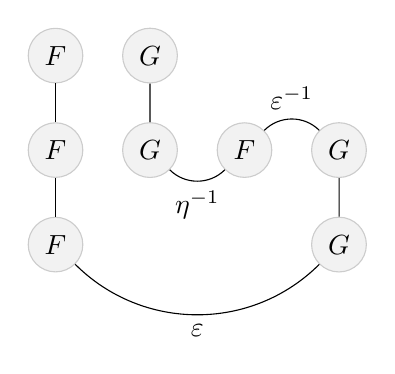
\begin{tikzpicture}[baseline=(X), scale=0.8, bend angle=45, auto, fct/.style={circle, draw=gray!40, fill=gray!10}, scale=1.5]
		\node[fct] (X0) at (0,1) {$F$};
		\node[fct] (X1) at (1,1) {$G$};

		\node[fct] (Y0) at (0,0) {$F$} edge (X0);
		\node[fct] (Y1) at (1,0) {$G$} edge (X1);
		\node[fct] (Y2) at (2,0) {$F$} edge[bend left] node {$\eta^{-1}$} (Y1);
		\node[fct] (Y3) at (3,0) {$G$} edge[bend right] node[swap] {$\varepsilon^{-1}$} (Y2);

		\node[fct] (Z0) at (0,-1) {$F$} edge (Y0);
		\node[fct] (Z1) at (3,-1) {$G$} edge (Y3) edge[bend left] node {$\varepsilon$} (Z0);
		\coordinate (X) at (0, -0.5);
	\end{tikzpicture} \quad = \quad 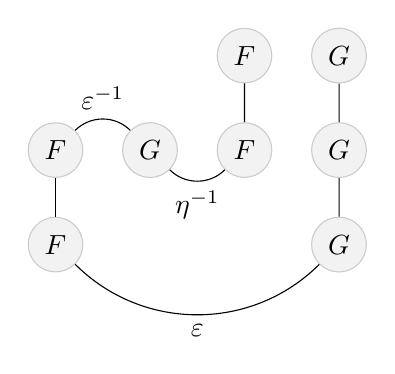
\begin{tikzpicture}[baseline=(X), scale=0.8, bend angle=45, auto, fct/.style={circle, draw=gray!40, fill=gray!10}, scale=1.5]
		\node[fct] (X0) at (2,1) {$F$};
		\node[fct] (X1) at (3,1) {$G$};

		\node[fct] (Y0) at (0,0) {$F$};
		\node[fct] (Y1) at (1,0) {$G$} edge[bend right] node[swap] {$\varepsilon^{-1}$} (Y0);
		\node[fct] (Y2) at (2,0) {$F$} edge[bend left] node {$\eta^{-1}$} (Y1) edge (X0);
		\node[fct] (Y3) at (3,0) {$G$} edge (X1);
	
		\node[fct] (Z0) at (0,-1) {$F$} edge (Y0);
		\node[fct] (Z1) at (3,-1) {$G$} edge (Y3) edge[bend left] node {$\varepsilon$} (Z0);
		\coordinate (X) at (0, -0.5);
	\end{tikzpicture} \end{equation}
	Diagram kiri memang merupakan penggambaran dari $\varepsilon \cdot (F\eta^{-1}G) \cdot (FG\varepsilon^{-1})$, sebab $FG\varepsilon^{-1}$ tidak lain ialah $\varepsilon^{-1}$ yang dikomposisikan secara horizontal di sebelah kiri oleh $\identity_F$ dan $\identity_G$, dan demikian seterusnya. Untuk beralih ke diagram kanan, gambarkan $FG \varepsilon^{-1}: FG \to FGFG$ sebagai berikut:
	\[ \begin{tikzpicture}[baseline=(X), bend angle=70, auto, fct/.style={circle, draw=gray!40, fill=gray!10}]
		\node[fct] (X0) {$F$}; \node[fct] (X1) [right=of X0] {$G$};
		\node[fct] (Y0) [below=of X0] {$F$} edge (X0); \node[fct] (Y1) [below=of X1] {$G$} edge (X1);
		\node[fct] (Y2) [right=of Y1] {$F$};
		\node[fct] (Y3) [right=of Y2] {$G$} edge[bend right] node {$\varepsilon^{-1}$} (Y2);
		\coordinate (X) at ($(X0)!.5!(Y0)$);
	\end{tikzpicture} = \begin{tikzpicture}[baseline=(X), bend angle=70, auto, fct/.style={circle, draw=gray!40, fill=gray!10}]
		\node[fct] (X0) {$F$}; \node[fct] (X1) [right=of X0] {$G$} edge[bend left] node[swap] {$\varepsilon$} (X0);
		\node[fct] (Y0) [below=of X0] {$F$}; \node[fct] (Y1) [below=of X1] {$G$} edge[bend right] node {$\varepsilon^{-1}$} (Y0);
		\node[fct] (Y2) [right=of Y1] {$F$};
		\node[fct] (Y3) [right=of Y2] {$G$} edge[bend right] node {$\varepsilon^{-1}$} (Y2);
		\coordinate (X) at ($(X0)!.5!(Y0)$);
	\end{tikzpicture} \]
	Karena komposisi horizontal dengan fungtor identitas tidak menimbulkan perubahan, $\varepsilon$ pada lapisan atas dapat ditempatkan di sebelah kiri ataupun kanan. Dengan demikian, diagram kanan menyederhana menjadi
	\[ \begin{tikzpicture}[baseline=(X), bend angle=70, auto, fct/.style={circle, draw=gray!40, fill=gray!10}]
		\node[fct] (X0) {$F$}; \node[fct] (X1) [right=of X0] {$G$} edge[bend left] node[swap] {$\varepsilon$} (X0);
		\node[fct] (Y0) [below=of X0] {$F$}; \node[fct] (Y1) [below=of X1] {$G$} edge[bend right] node {$\varepsilon^{-1}$} (Y0);
		\node[fct] (Y3) [left=of Y0] {$G$};
		\node[fct] (Y2) [left=of Y3] {$F$} edge[bend left] node {$\varepsilon^{-1}$} (Y3);
		\coordinate (X) at ($(X0)!.5!(Y0)$);
	\end{tikzpicture} = \begin{tikzpicture}[baseline=(X), bend angle=70, auto, fct/.style={circle, draw=gray!40, fill=gray!10}]
		\node[fct] (X0) {$F$}; \node[fct] (X1) [right=of X0] {$G$};
		\node[fct] (Y0) [below=of X0] {$F$} edge (X0); \node[fct] (Y1) [below=of X1] {$G$} edge (X1);
		\node[fct] (Y3) [left=of Y0] {$G$};
		\node[fct] (Y2) [left=of Y3] {$F$} edge[bend left] node {$\varepsilon^{-1}$} (Y3);
		\coordinate (X) at ($(X0)!.5!(Y0)$);
	\end{tikzpicture} \]
	Dengan menambahkan $\varepsilon \cdot (F\eta^{-1}G)$ di bawah ruas kanan, kita memperoleh \eqref{eqn:adj-equiv-two-expression}.

	Sekarang kita buktikan \eqref{eqn:adj-zigzag-2}. Substitusikan diagram kiri dalam \eqref{eqn:adj-equiv-two-expression} untuk $\varepsilon'$; dengan menghilangkan label fungtor, $(G\varepsilon')(\eta G)$ dapat digambarkan sebagai
	\[ 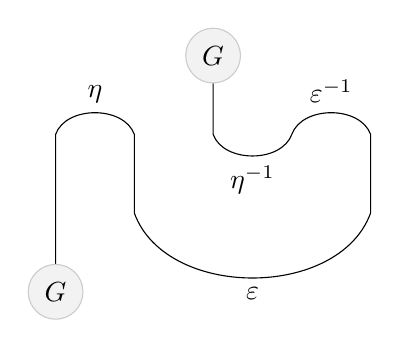
\begin{tikzpicture}[baseline=(X), bend angle=70, auto, fct/.style={circle, draw=gray!40, fill=gray!10}]
		\coordinate (A) at (0,0); \coordinate (B) at (0,2); \coordinate (C) at (1,2); \coordinate (D) at (1,1); \coordinate (E) at (4,1); \coordinate (F) at (4,2); \coordinate (G) at (3,2); \coordinate (H) at (2,2); \coordinate (I) at (2,3);
	
		\draw (A) -- (B) to[bend left] node {$\eta$} (C) -- (D) to[bend right] node[swap] {$\varepsilon$} (E) -- (F) to[bend right] node[swap] {$\varepsilon^{-1}$} (G) to[bend left] node {$\eta^{-1}$} (H) -- (I);
	
		\node[fct] at (A) {$G$}; \node[fct] at (I) {$G$};
		\coordinate (X) at (0, 1.5);
	\end{tikzpicture} \quad = \quad
	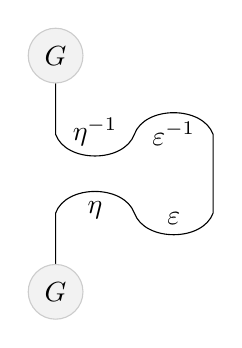
\begin{tikzpicture}[baseline=(X), bend angle=70, auto, fct/.style={circle, draw=gray!40, fill=gray!10}]
		\coordinate (A) at (0,0); \coordinate (B) at (0,1); \coordinate (C) at (1,1); \coordinate (D) at (2,1); \coordinate (E) at (2,2); \coordinate (F) at (1,2); \coordinate (G) at (0,2); \coordinate (H) at (0,3);
	
		\draw (A) -- (B) to[bend left] node[swap] {$\eta$} (C) to[bend right] node {$\varepsilon$} (D) -- (E) to[bend right] node {$\varepsilon^{-1}$} (F) to [bend left] node[swap] {$\eta^{-1}$} (G) -- (H);
		\node[fct] at (A) {$G$}; \node[fct] at (H) {$G$};
		\coordinate (X) at (0, 1.5);
	\end{tikzpicture}\]
	Untuk mengubah diagram kiri menjadi diagram kanan, mula-mula rentangkan diagram itu secara vertikal (yakni, sisipkan $\identity_F$, $\identity_G$, dan seterusnya di tengah), kemudian geser $\eta^{-1}$ ke kiri; alasannya serupa dengan argumen bagi \eqref{eqn:adj-equiv-two-expression}. Sekarang, dengan menggunakan $\eta \eta^{-1} = \identity_{GF}$ dan $\varepsilon^{-1}\varepsilon = \identity$, diagram kanan dapat disederhanakan menjadi
	\[\begin{tikzpicture}[baseline=(X), bend angle=70, auto, fct/.style={circle, draw=gray!40, fill=gray!10}]
		\node[fct] (A) {$G$}; \node[fct] (B) [above=of A] {$G$} edge (A);
		\node[fct] (C) [right=of A] {$F$}; \node[fct] (D) [above=of C] {$F$} edge (C);
		\node[fct] (E) [right=of C] {$G$} edge[bend left] node[swap] {$\varepsilon$} (C);
		\node[fct] (F) [right=of D] {$G$} edge[bend right] node {$\varepsilon^{-1}$} (D) edge (E);
		\coordinate (X) at ($(A)!.5!(B)$);
	\end{tikzpicture} \quad = \quad \begin{tikzpicture}[baseline=(X), bend angle=70, auto, fct/.style={circle, draw=gray!40, fill=gray!10}]
		\node[fct] (A) {$G$}; \node[fct] (B) [above=of A] {$G$} edge (A);
		\coordinate (X) at ($(A)!.5!(B)$);
	\end{tikzpicture}\]
	Ini membuktikan \eqref{eqn:adj-zigzag-2}. Kasus \eqref{eqn:adj-zigzag-1} hampir merupakan bayangan cermin dari argumen di atas; satu-satunya perbedaan ialah kita menggunakan diagram kanan dalam \eqref{eqn:adj-equiv-two-expression} untuk menggantikan $\varepsilon'$.
	
		Terakhir, kita buktikan keunikannya. Andaikan $\varepsilon'': FG \to \identity$ juga memenuhi \eqref{eqn:adj-zigzag-1} dan \eqref{eqn:adj-zigzag-2}. Perhatikan bahwa $\varepsilon''\cdot (\varepsilon' FG) = \varepsilon' \cdot (FG \varepsilon'')$; hal ini karena keduanya bersesuaian dengan diagram yang sama, $FGFG \to \identity$:
	\[\begin{tikzpicture}[baseline=(X), bend angle=45, auto, fct/.style={circle, draw=gray!40, fill=gray!10}]
		\node[fct] (F) {$F$}; \node[fct] (G) [right=of F] {$G$} edge[bend left] node[swap] {$\varepsilon'$} (F);
		\node[fct] (F1) [right=of G] {$F$}; \node[fct] (G1) [right=of F1] {$G$} edge[bend left] node[swap] {$\varepsilon''$} (F1);
		\coordinate (X) at (F);
	\end{tikzpicture}.\]
	Selain itu, mudah dilihat bahwa $(\varepsilon'F \cdot F\eta)G = \varepsilon' FG \cdot F\eta G$ dan $F(G\varepsilon'' \cdot \eta G) = FG\varepsilon'' \cdot F\eta G$. Dengan menerapkan \eqref{eqn:adj-zigzag-1} dan \eqref{eqn:adj-zigzag-2}, keduanya sama dengan $\identity_{FG}$. Oleh karena itu, $\varepsilon'' = \varepsilon'' \cdot (\varepsilon' FG) (F\eta G) = \varepsilon' (FG\varepsilon'')(F\eta G) = \varepsilon'$. Keunikan pun terbukti.
\end{proof}

Dalam teori kategori masih terdapat banyak teknik visualisasi serupa. Pembaca dapat merujuk kepada survei yang ditulis P.\ Selinger dalam \cite[Chapter 4]{Co11}. Teknik serupa akan kita jumpai lagi dalam \S\ref{sec:braiding}.
	
\section{Limit}\label{sec:limits}
Pertama-tama kita berikan definisi umum limit, lalu menguraikannya secara bertahap.

\begin{definition}\label{def:diagonal-functor}
	Misalkan $I, \mathcal{C}$ kategori. Definisikan fungtor diagonal $\Delta: \mathcal{C} \to \mathcal{C}^I := \text{Fct}(I, \mathcal{C})$ sebagai berikut: fungtor ini memetakan setiap $X \in \Obj(\mathcal{C})$ ke fungtor konstan
	\begin{gather*}
		\Delta(X): I \longrightarrow \mathcal{C}\;
		\left\{ \begin{array}{ll}
			\forall i \in \Obj(I), & i \longmapsto X \\
			\forall [i \to j] \in \Mor(I), & [i \to j] \longmapsto [\identity_X: X \to X].
		\end{array}\right.
	\end{gather*}
	Untuk morfisme $f: X \to Y$ yang diberikan, dalam kategori $\mathcal{C}^I$ definisi $\Delta(f): \Delta(X) \to \Delta(Y)$ sudah jelas: pada setiap $i \in \Obj(I)$, komponennya adalah $f: X \to Y$.
\end{definition}

Dengan memakai $I^{\text{op}}$ sebagai pengganti $I$, dapat pula didefinisikan fungtor diagonal $\Delta: \mathcal{C} \to \mathcal{C}^{I^{\text{op}}} := \text{Fct}(I^{\text{op}}, \mathcal{C})$. Ingat Definisi \ref{def:comma-category} dan pembahasan sesudahnya: untuk fungtor $I \xrightarrow{\alpha} \mathcal{C} \xleftarrow{\beta} I^\text{op}$, dapat dibentuk dua kategori koma
\begin{align*}
	\left[ \mathbf{1} \xrightarrow{j_\alpha} \mathcal{C}^I \xleftarrow{\Delta} \mathcal{C} \right] & \leadsto \quad (j_\alpha/\Delta) =: (\alpha / \Delta), \\
	\left[ \mathcal{C} \xrightarrow{\Delta} \mathcal{C}^{I^\text{op}} \xleftarrow{j_\beta} \mathbf{1} \right] & \leadsto \quad (\Delta/j_\beta) =: (\Delta/\beta).
\end{align*}
\begin{definition}[Limit]\label{def:limit}\index{guinajixian@limit induktif (inductive limit)}\index{toushejixian@limit proyektif (projective limit)}\index[sym1]{limind@$\varinjlim$}\index[sym1]{limproj@$\varprojlim$}
	Misalkan $I, \mathcal{C}$ kategori. Pertimbangkan fungtor $\alpha: I \to \mathcal{C}$ dan $\beta: I^\text{op} \to \mathcal{C}$.
	\begin{compactenum}
		\item Jika kategori koma $(\alpha / \Delta)$ mempunyai objek awal, objek itu dinotasikan dengan $\varinjlim \alpha$ dan disebut \emph{limit induktif} dari $\alpha$;
		\item Jika kategori koma $(\Delta / \beta)$ mempunyai objek terminal, objek itu dinotasikan dengan $\varprojlim \beta$ dan disebut \emph{limit proyektif} dari $\beta$.
	\end{compactenum}
	Keduanya juga disebut limit berindeks $I$.
\end{definition}
Terminologi tentang limit belum seragam; berikut beberapa versi yang lazim.
\begin{center}\begin{tabular}{c|c}
	$\varinjlim$ & $\varprojlim$ \\
	Limit induktif & Limit proyektif \\
	Limit langsung & Limit invers \\
	Kolimit ($\text{colim}$) & Limit ($\text{lim}$)
\end{tabular}\end{center}

Proposisi \ref{prop:initial-obj-uniqueness} menjamin bahwa setiap limit, jika ada, bersifat unik. Lebih tepatnya, kategori koma memberikan deskripsi berikut berdasarkan diagram komutatif dalam $\mathcal{C}$
\begin{equation*}\begin{gathered}
	(\alpha/\Delta): \left\{ \begin{array}{ll}
		\text{objek}: & \left( L, (\alpha(i) \xrightarrow{f_i} L)_{i \in \Obj(I)} \right), \quad \forall\; [i \xrightarrow{\phi} j], \;
			\begin{tikzcd}[column sep=tiny, row sep=tiny]
				\alpha(i) \arrow[rd] \arrow[rr, "{\alpha(\phi)}"] & & \alpha(j) \arrow[ld] \\
				{} & L &
			\end{tikzcd} \\
		\text{morfisme}: & \left[ \varphi: (L, (f_i)_i) \to (L', (f'_i)_i) \right] =  \forall i, \;
			\begin{tikzcd}[column sep=tiny, row sep=small]
				\alpha(i) \arrow[r, "f_i"] \arrow[rd, "f'_i"'] & L \arrow[d, "\varphi"] \\
				{} & L'
			\end{tikzcd}
	\end{array}\right. \\
	(\Delta/\beta): \left\{ \begin{array}{ll}
		\text{objek}: & \left( L, (L \xrightarrow{g_i} \beta(i))_{i \in \Obj(I)} \right), \quad \forall\; [i \xrightarrow{\phi} j], \;
			\begin{tikzcd}[column sep=tiny, row sep=tiny]
				\beta(i) & & \beta(j) \arrow[ll, "\beta(\phi)"'] \\
				{} & L \arrow[lu] \arrow[ru] &
			\end{tikzcd} \\
		\text{morfisme}: & \left[ \varphi: (L, (g_i)_i) \to (L', (g'_i)_i) \right] =  \forall i, \;
			\begin{tikzcd}[column sep=tiny, row sep=small]
				\beta(i) & L \arrow[d, "\varphi"] \arrow[l, "g_i"'] \\
				{} & L' \arrow[lu, "g'_i"]
			\end{tikzcd}
	\end{array}\right.
\end{gathered}\end{equation*}

Dalam beberapa pustaka, objek dari $(\alpha/\Delta)$ dan $(\Delta/\beta)$ masing-masing disebut kerucut dan kokerucut; sebutan ini bersifat intuitif.

Dengan demikian, limit induktif dari $\alpha$ dapat dipahami kembali sebagai data $(\varinjlim \alpha, \alpha(i) \xrightarrow{\iota_i} \varinjlim \alpha)$, sedangkan limit proyektif dari $\beta$ sebagai data $(\varprojlim \beta, \varprojlim \beta \xrightarrow{p_i} \beta(i))$; sifat universal masing-masing digambarkan oleh
\begin{equation}\label{eqn:lim-diagrams}\begin{tikzcd}
	\alpha(i) \arrow[rd, "{\iota_i}"] \arrow[rdd] \arrow[rr, "{\alpha(\phi)}"] & & \alpha(j) \arrow[ld, "{\iota_j}"'] \arrow[ldd] \\
	& \varinjlim \alpha \arrow[dashed, d, "\exists !"] &  \\
	& L &
	\end{tikzcd}\quad\begin{tikzcd}
	\beta(i) & & \beta(j) \arrow[ll, "{\beta(\phi)}"'] \\
	& \varprojlim \beta \arrow[lu, "p_i"'] \arrow[ru, "p_j"] & \\
	& L \arrow[luu] \arrow[ruu] \arrow[dashed, u, "{\exists !}"'] &
\end{tikzcd}\end{equation}
Diagram tersebut dibaca sebagai berikut: untuk setiap objek dari $(\alpha / \Delta)$ atau $(\Delta/\beta)$ yang berbentuk $(L, \ldots)$, terdapat morfisme tunggal $\dashrightarrow$ sehingga seluruh diagram komutatif untuk setiap $\phi \in \Mor(I)$.

\begin{remark}\label{rem:lim-duality}
	Perhatikan bahwa arah panah pada kedua diagram dalam \eqref{eqn:lim-diagrams} saling berlawanan. Sesungguhnya, $\varinjlim$ dan $\varprojlim$ adalah konsep dual: misalkan $\alpha: I \to \mathcal{C}$; pada kategori lawan terdapat $\alpha^\text{op}: I^\text{op} \to \mathcal{C}^\text{op}$ yang bersesuaian (Catatan \ref{rem:op-functor}). Untuk $I^\text{op}$ dan $\mathcal{C}^\text{op}$ terdapat pula fungtor diagonal $\Delta^{\text{op}}$ yang bersesuaian. Dengan demikian diperoleh
	\begin{align*}
		(\alpha / \Delta)^\text{op} & = (\Delta^\text{op} / \alpha^\text{op}), \\
		\varprojlim (\alpha^{\text{op}}) & = \varinjlim \alpha, \quad \text{jika limit pada salah satu ruas ada}.
	\end{align*}
\end{remark}

\begin{lemma}\label{prop:lim-functoriality}
	Misalkan $\psi: \alpha \to \alpha'$ suatu morfisme dalam kategori fungtor $\mathcal{C}^I$. Andaikan semua $\varinjlim$ yang bersesuaian ada. Maka terdapat morfisme tunggal $\varinjlim \psi$ sedemikian sehingga
	\begin{tikzcd}[row sep=small, column sep=small]
		\alpha(i) \arrow[r] \arrow[d, "\psi(i)"'] & \varinjlim \alpha \arrow[d, "\varinjlim\psi"] \\
		\alpha'(i) \arrow[r] & \varinjlim \alpha'
	\end{tikzcd}
	komutatif untuk setiap $i$. Jika $\alpha \xrightarrow{\psi_1} \alpha' \xrightarrow{\psi_2} \alpha''$, maka $\varinjlim (\psi_2 \psi_1) = \varinjlim \psi_2 \varinjlim \psi_1$. Hasil serupa juga berlaku untuk $\varprojlim$: secara natural, $\psi: \beta \to \beta'$ menginduksi $\varprojlim \beta \to \varprojlim \beta'$, dan seterusnya.
\end{lemma}
\begin{proof}
	Dalam sifat universal $\varinjlim \alpha$, cukup ambil $L := \varinjlim \alpha' \leftarrow \alpha'(i) \xleftarrow{\psi(i)} \alpha(i)$. Sifat $\varinjlim (\psi_2 \psi_1) = \varinjlim \psi_2 \varinjlim \psi_1$ mengikuti dari
	\[\begin{tikzcd}[row sep=small, column sep=small]
		\alpha(i) \arrow[r] \arrow[d] & \alpha'(i) \arrow[r] \arrow[d] & \alpha''(i) \arrow[d] \\
		\varinjlim \alpha \arrow[r] & \varinjlim \alpha' \arrow[r] & \varinjlim \alpha''
	\end{tikzcd} \qquad i \in \Obj(I) \]
	komutativitas seluruh diagram.
\end{proof}

Selanjutnya kita mengikuti Konvensi \ref{con:U-small} dan membedakan kategori dari kategori kecil. Kita hanya mempertimbangkan limit dengan $I$ kategori kecil. Hal ini terutama demi kemudahan perumusan; lagi pula, menurut Hipotesis \ref{hyp:universe}, semesta $\mathcal{U}$ yang dipilih selalu dapat diperbesar agar semua kategori yang dibahas menjadi kategori kecil. Namun, pembaca tetap perlu waspada karena dalam beberapa situasi ukuran himpunan benar-benar dapat menimbulkan perbedaan substantif, seperti dalam Proposisi \ref{prop:preorder-complete} yang akan disebutkan di bawah.

\begin{example}\label{eg:set-limits}
	Ambil $\mathcal{C} := \cate{Set}$ dan misalkan $I$ kategori kecil. Pertama-tama kita konstruksikan $\varprojlim \beta$. Definisikan
	\begin{align*}
		\varprojlim \beta & := \left\{ (x_i)_{i \in \Obj(I)} \in \prod_i \beta(i) : \forall \sigma \in \Hom_I(i,j), \; \beta(\sigma)(x_j) = x_i \right\} \\
		& = \Ker\left[ \prod_i \beta(i) \rightrightarrows \prod_\sigma \beta(s(\sigma)) \right] \quad \text{(ekualiser)},
	\end{align*}
	Kedua panah dalam $\Ker[\cdots]$ masing-masing memiliki pemetaan $(x_i)_i \mapsto x_{s(\sigma)}$ dan $(x_i)_i \mapsto \beta(\sigma)\left(x_{t(\sigma)}\right)$ sebagai ``koordinat-$\sigma$''-nya, dengan $\sigma$ merentang semua morfisme dalam $I$. Ekspresi di atas merupakan sebuah objek dalam $\cate{Set}$ dan dilengkapi keluarga pemetaan proyeksi $p_j: \varprojlim \beta \to \beta(j)$, $p_j((x_i)_i) = x_j$, dengan $j$ merentang $\Obj(I)$. Tidak sulit memeriksa bahwa $(\varprojlim \beta, (p_j)_j)$ adalah limit proyektif dari $\beta$.

	Selanjutnya, pertimbangkan $\alpha: I \to \cate{Set}$. Definisikan
	\[ \varinjlim \alpha := \left( \bigsqcup_{i \in \Obj(I)} \alpha(i) \right) \Big/ \sim \]
	dengan $\bigsqcup_i \alpha(i)$ menyatakan gabungan saling lepas, sedangkan $\sim$ adalah relasi ekuivalensi yang dibangkitkan oleh relasi berikut
	\[ x \sim \alpha(\sigma)(x), \quad \sigma: i \to j, \quad x \in \alpha(i). \]
	Dari sifat himpunan hasil bagi diperoleh keluarga pemetaan $\iota_j: \alpha(j) \to \varinjlim \alpha$, dengan $j$ merentang $\Obj(I)$; pemetaan ini membawa $x \in \alpha(j)$ ke kelas ekuivalensi yang memuat $x$. Tidak sulit memeriksa bahwa $(\varinjlim \alpha, (\iota_j)_j)$ adalah limit induktif dari $\alpha$.
\end{example}
Konstruksi di atas memiliki satu kekurangan yang jelas: konstruksi itu hanya menjelaskan cara ``membangkitkan'' relasi ekuivalensi $\sim$, tetapi tidak memberikan deskripsi langsung. Untuk mengatasinya, diperlukan syarat tambahan pada $I$; pada saat yang sama kita perkenalkan konsep kategori terarah ke atas.

\begin{definition}\label{def:filtrant-cat}\index{luguofanchou@kategori terarah ke atas (filtered category)}
	Kategori tak kosong $I$ disebut \emph{terarah ke atas (filtered)} jika memenuhi syarat-syarat berikut:
	\begin{compactitem}
		\item Untuk setiap $i, j \in \Obj(I)$, terdapat $k \in \Obj(I)$ dan morfisme $i \to k$, $j \to k$;
		\item Untuk setiap panah $f,g: i \to j$, terdapat $k \in \Obj(I)$ dan $h: j \to k$ sedemikian sehingga $hf = hg$.
	\end{compactitem}
\end{definition}
Untuk kategori yang berasal dari poset tak kosong $(I, \leq)$, syarat kedua bersifat mubazir; dalam hal ini kita kembali pada konsep poset terarah ke atas (filtered poset) yang didefinisikan dalam \S\ref{sec:group-limit}. Sebagai contoh, poset $(\Z_{\geq 1}, \leq)$ adalah poset terarah ke atas.

Sekarang kembali ke Contoh \ref{eg:set-limits}, yakni fungtor $\alpha: I \to \cate{Set}$, dan andaikan $I$ terarah ke atas. Pada gabungan saling lepas $\bigsqcup_{i \in \Obj(I)} \alpha(i)$, definisikan relasi $\sim$ sebagai berikut: untuk setiap $i, j \in \Obj(I)$ serta $x_i \in \alpha(i)$, $x_j \in \alpha(j)$, jika
\begin{equation}\label{eqn:filtrant-equiv} \text{terdapat} \begin{cases}
	f: i \to k, \\
	g: j \to k
	\end{cases}
	\text{sedemikian sehingga} \quad \alpha(f)(x_i) = \alpha(g)(x_j) \in \alpha(k)
\end{equation}
maka tetapkan $x_i \sim x_j$. Jelas bahwa relasi ekuivalensi dalam Contoh \ref{eg:set-limits} juga harus memenuhi sifat ini. Jika dapat ditunjukkan bahwa $\sim$ sudah merupakan relasi ekuivalensi, maka $\sim$ di sini tepat sama dengan relasi dalam Contoh \ref{eg:set-limits} yang juga dinotasikan $\sim$. Refleksivitas dan simetrinya jelas; kini kita periksa transitivitasnya. Andaikan $(x_i \sim x_j) \wedge (x_j \sim x_k)$; terdapat diagram
\[ \begin{tikzcd}[scale=0.75]
	i \arrow[rd] & & j \arrow[ld] \arrow[rd] & & k \arrow[ld] \\
	& h \arrow[dashed, rd] & & h' \arrow[dashed, ld] & \\
	& & g & &
\end{tikzcd} \quad \begin{tikzcd}[scale=0.75]
	x_i \arrow[mapsto, rd] & & x_j \arrow[mapsto, ld] \arrow[mapsto, rd] & & x_k \arrow[mapsto, ld] \\
	& x_h \arrow[dashed, rd] & & x_{h'} \arrow[dashed, mapsto, ld] & \\
	& & ? & & 
\end{tikzcd} \]
Panah putus-putus dan $g$ di dalamnya dilengkapi dengan syarat pertama Definisi \ref{def:filtrant-cat}. Akan tetapi, citra $x_h$ dan $x_{h'}$ di bawah panah putus-putus belum tentu sama. Karena itu, dengan syarat kedua definisi tersebut, kita cari dalam $I$ suatu morfisme $g \to g'$ sehingga morfisme komposit $j \to h \to g \to g'$ sama dengan $j \to h' \to g \to g'$. Dengan memakai $g'$ sebagai pengganti $g$ dalam diagram, dapat dipastikan bahwa $x_i \sim x_k$. Jadi, $\sim$ merupakan relasi ekuivalensi. Dari definisi $\sim$ juga diperoleh komutativitas diagram kiri dalam \eqref{eqn:lim-diagrams}. Ringkasnya,
\[ \varinjlim \alpha := \bigsqcup_{i \in \Obj(I)} \alpha(i) \big/ \sim \]
Kelak kita akan berulang kali mempertimbangkan $\varinjlim$ berindeks kategori terarah ke atas dalam berbagai kategori.

\begin{example}\label{eg:top-limits}
	Dengan cara yang sama dapat dikonstruksikan limit dalam kategori $\mathcal{C} := \cate{Top}$. Untuk kategori kecil $I$, konstruksi limit $(\varinjlim \alpha, \iota_j)$ dan $(\varprojlim \beta, p_j)$ persis sama dengan konstruksi dalam $\cate{Set}$; kita hanya perlu melengkapi himpunan-himpunan tersebut dengan topologi hasil bagi atau topologi subruang \cite[\S 3.1, \S 3.4]{Xiong}.
\end{example}

Misalkan kategori $\mathcal{C}$ diberikan. Meskipun limit yang dibahas belum tentu ada dalam $\mathcal{C}$, setelah $\mathcal{C}$ dibenamkan ke kategori fungtor $\mathcal{C}^\wedge$ atau $\mathcal{C}^\vee$ (lihat \S\ref{sec:representable-functors}), keberadaan semua limit (kecil) dapat dijamin.

\begin{proposition}\label{prop:lim-Yoneda}
	Misalkan $I$ kategori kecil. Limit fungtor $\alpha: I \to \mathcal{C}^\wedge$ diberikan oleh objek $\Yinjlim \alpha \in \Obj(\mathcal{C}^\wedge)$ yang didefinisikan sebagai berikut:
	\begin{gather*}
		\Yinjlim \alpha: S \longmapsto \varinjlim \left( \alpha(S) \right), \\
		[T \xrightarrow{f} S] \leadsto \varinjlim \alpha(S) \xrightarrow{\varinjlim \alpha(f)} \varinjlim \alpha(T),
	\end{gather*}
	beserta keluarga transformasi natural $\alpha(j)(\cdot) \to \varinjlim \alpha(\cdot)$, dengan $j \in \Obj(I)$ dan konstruksi $\varinjlim \alpha(f)$ diberikan dalam Lema \ref{prop:lim-functoriality}; di sini $\varinjlim$ tanpa hiasan tambahan adalah limit dalam $\cate{Set}$. Demikian pula, limit fungtor $\beta: I^\text{op} \to \mathcal{C}^\wedge$ diberikan oleh
	\[ \Yprojlim \beta: S \longmapsto \varprojlim \left( \beta(S) \right) \]
	dan data-data serupa. Sifat serupa juga berlaku bagi kasus dengan nilai dalam $\mathcal{C}^\vee$; secara notasi, semua limit ini kita tulis tanpa membedakannya sebagai
	\begin{align*}
		\Yinjlim \alpha: S & \longmapsto \varinjlim \left( \alpha(S) \right), \quad \alpha: I \to \mathcal{C}^\wedge \;\text{atau}\; \mathcal{C}^\vee, \\
		\Yprojlim \beta: S & \longmapsto \varprojlim \left( \beta(S) \right), \quad \beta: I^\text{op} \to \mathcal{C}^\wedge \;\text{atau}\; \mathcal{C}^\vee.
	\end{align*}
\end{proposition}
\begin{proof}
	Caranya ialah mengambil limit fungtor secara titik demi titik (atau objek demi objek), sehingga kasusnya tereduksi ke $\cate{Set}$. Kita hanya uraikan kasus $\alpha: I \to \mathcal{C}^\wedge$ dan $\Yinjlim \alpha$. Pertimbangkan diagram \eqref{eqn:lim-diagrams} yang bersesuaian, serta berikan $L \in \mathcal{C}^\wedge$ dan keluarga morfisme $\alpha(i) \to L$. Untuk setiap $S \in \Obj(\mathcal{C})$, konstruksi dalam $\cate{Set}$ bagi $\varinjlim$ menunjukkan bahwa terdapat $\varphi(S)$ tunggal sehingga diagram
	\begin{tikzcd}[column sep=tiny, row sep=tiny]
		\alpha(i)(S) \arrow[rr] \arrow[rd] & & \varinjlim \alpha(S) \arrow[ld, "\varphi(S)"] \\
		& L(S) &
	\end{tikzcd}
	komutatif untuk semua $i$. Kuncinya ialah membuktikan bahwa semua $\varphi(\cdot)$ ini dapat, dalam $\mathcal{C}^\wedge$, dirangkai menjadi $\Yinjlim \alpha \xrightarrow{\varphi} L$. Pertimbangkan dalam $\mathcal{C}$ sebarang morfisme $f: T \to S$. Selanjutnya, pandang $L(S)$ sebagai fungtor konstan $\Delta(L(S)): I \to \cate{Set}$; mudah dilihat bahwa $\varinjlim$-nya adalah $L(S)$ sendiri (silakan periksa). Demikian pula untuk $L(T)$. Maka, dari Lema \ref{prop:lim-functoriality} diperoleh: untuk setiap $i \in \Obj(I)$,
	\[ \begin{tikzcd}
		\alpha(i)(S) \arrow[r, "\alpha(i)(f)"] \arrow[d] & \alpha(i)(T) \arrow[d] \\
		L(S) \arrow[r, "L(f)"'] & L(T)
	\end{tikzcd} \;\text{komutatif, sehingga} \;
	\begin{tikzcd}
		\varinjlim \alpha(S) \arrow[r, "{\varinjlim \alpha(f)}", yshift=0.5em] \arrow[d, "\varphi(S)"'] & \varinjlim \alpha(T) \arrow[d, "\varphi(T)"] \\
		L(S) \arrow[r, "L(f)"'] & L(T)
	\end{tikzcd} \;\text{komutatif}, \]
	dan diagram kanan tepat menyatakan fungtorialitas yang diperlukan oleh $\varphi(\cdot)$.
\end{proof}
Dengan demikian, keberadaan limit tereduksi pada representabilitas fungtor; lihat \S\ref{sec:representable-functors}.

\begin{proposition}\label{prop:lim-as-fct}
	Misalkan $I$ kategori kecil. Berikut ini kita menggunakan fungtor $k_{\mathcal{C}}$ dan $h_{\mathcal{C}}$ untuk memandang $\mathcal{C}$ masing-masing sebagai subkategori dari $\mathcal{C}^\vee$ dan $\mathcal{C}^\wedge$.
	\begin{enumerate}
		\item Limit induktif fungtor $\alpha: I \to \mathcal{C}$ ada jika dan hanya jika $\Yinjlim \alpha \in \mathcal{C}^\vee$ representabel; memberikan limit dari $\alpha$ ekuivalen dengan memberikan objek $\varinjlim \alpha \in \Obj(\mathcal{C})$ beserta isomorfisme $k_{\mathcal{C}}(\varinjlim \alpha) \rightiso \Yinjlim \alpha$.
		\item Limit proyektif fungtor $\beta: I^\text{op} \to \mathcal{C}$ ada jika dan hanya jika $\Yprojlim \beta \in \mathcal{C}^\wedge$ representabel; memberikan limit dari $\beta$ ekuivalen dengan memberikan objek $\varprojlim \beta \in \Obj(\mathcal{C})$ beserta isomorfisme $h_{\mathcal{C}}(\varprojlim \beta) \rightiso \Yprojlim \beta$.
	\end{enumerate}
\end{proposition}
Sifat limit dengan demikian dapat dicirikan secara ringkas sebagai
\begin{align*}
	\Hom_{\mathcal{C}}(\varinjlim \alpha, \cdot) & \rightiso \varprojlim_i \Hom_{\mathcal{C}}(\alpha(i), \cdot) = \Yinjlim \alpha, \\
	\Hom_{\mathcal{C}}(\cdot, \varprojlim \beta) & \rightiso \varprojlim_i \Hom_{\mathcal{C}}(\cdot, \beta(i)) = \Yprojlim \beta.
\end{align*}
Perhatikan bahwa $\mathcal{C}^\vee$ dan $\mathcal{C}^\wedge$ di sini tidak dapat dipertukarkan: limit di luar $\Hom_{\mathcal{C}}$ haruslah $\varprojlim$!

\begin{proof}
	Pertama, tinjau kasus limit induktif. Sifat universal dalam \eqref{eqn:lim-diagrams} dapat ditulis ulang sebagai berikut: memberikan limit dari $\alpha$ ekuivalen dengan memberikan objek $\varinjlim \alpha \in \Obj(\mathcal{C})$ beserta keluarga morfisme $\iota_i: \alpha(i) \to \varinjlim \alpha$, sedemikian sehingga morfisme antarfungtor
	\begin{equation*}\begin{tikzcd}[row sep=small]
		k_{\mathcal{C}}(\varinjlim \alpha) \arrow[equal, r] & \Hom_{\mathcal{C}}(\varinjlim \alpha , \cdot) \arrow[r, "\xi"] & \varprojlim_i \Hom_{\mathcal{C}}(\alpha(i), \cdot) & \Yinjlim \alpha \arrow[equal, l] \\
		& f \arrow[phantom, u, sloped, "\in" description] \arrow[mapsto, r] & (\iota_i^* f = f \circ \iota_i)_{i \in \Obj(I)} \arrow[phantom, u, sloped, "\in" description] &
	\end{tikzcd}\end{equation*}
	merupakan isomorfisme. Sebaliknya, setiap isomorfisme $\xi: k_{\mathcal{C}}(\varinjlim \alpha) \rightiso \Yinjlim \alpha$ dapat diinduksi dengan cara tersebut oleh suatu keluarga $\iota_i: \alpha(i) \to \varinjlim \alpha$: ini merupakan penerapan Teorema \ref{prop:Yoneda-lemma}. Secara lebih langsung, ambil peubah pada diagram di atas sebagai $\varinjlim \alpha$; citra dari $f = \identity$ tepat merupakan $(\iota_i)_i$ yang dicari.

	Kasus limit proyektif ditangani dengan cara yang sepenuhnya serupa; kali ini isomorfisme yang ditinjau ialah
	\begin{equation*}\begin{tikzcd}[row sep=small]
		\Hom_{\mathcal{C}}(\cdot, \varprojlim \beta) \arrow[r] & \varprojlim_i \Hom_{\mathcal{C}}(\cdot, \beta(i)) = \Yprojlim \beta \\
		f \arrow[phantom, u, sloped, "\in" description] \arrow[mapsto, r] & (p_{i *} f = p_i \circ f)_{i \in \Obj(I)} \arrow[phantom, u, sloped, "\in" description]
	\end{tikzcd}\end{equation*}
	Pernyataan pun terbukti.
\end{proof}

Proposisi \ref{prop:lim-as-fct} mereduksi banyak sifat limit ke kasus himpunan, sehingga pembuktiannya sangat disederhanakan. Mari kita lihat sebuah contoh.
\begin{lemma}\label{prop:lim-Fubini}
	Misalkan $I, J$ kategori kecil dan andaikan $\mathcal{C}$ memiliki limit induktif berindeks $I$ dan $J$, yang dinotasikan dengan $\varinjlim$. Pertimbangkan fungtor $\alpha: I \times J \to \mathcal{C}$. Terdapat isomorfisme kanonik
	\[ \varinjlim_j \left( \varinjlim\alpha(\cdot, j) \right) \simeq \varinjlim \alpha \simeq \varinjlim_i \left( \varinjlim\alpha(i, \cdot) \right) \]
	dengan limit pada ruas kiri diambil terlebih dahulu terhadap $I$, lalu terhadap $J$, sedangkan pada ruas kanan urutannya dibalik. Kasus limit proyektif $\varprojlim \beta$ serupa.
\end{lemma}
\begin{proof}
	Cukup buktikan kasus $\varinjlim$. Untuk suatu morfisme dalam $I$ yang diberikan, yakni $i \to i'$, Lema \ref{prop:lim-functoriality} memberikan diagram komutatif natural berikut untuk setiap $j$:
	\[ \begin{tikzcd}
		\varinjlim \alpha(i, \cdot) \arrow[r] & \varinjlim \alpha(i', \cdot) \\
		\alpha(i, j) \arrow[r] \arrow[u] & \alpha(i', j) \arrow[u]
	\end{tikzcd} \]
	Karena itu, limit pada ruas kanan dalam pernyataan tersebut terdefinisi; demikian pula ruas kiri. Proposisi \ref{prop:lim-as-fct} mereduksi pernyataan itu ke kategori $\mathcal{C} = \cate{Set}$, tepatnya kasus $\varprojlim$, yang langsung jelas dari konstruksi pada Contoh \ref{eg:set-limits}.
\end{proof}

Jika himpunan objek dan himpunan morfisme kategori $I$ keduanya berhingga, limit yang bersesuaian disebut limit berhingga; dalam hal ini, diagram lazim digunakan untuk mendeskripsikan konstruksi $I$. Limit dapat dikonstruksikan dalam dua tahap: produk (atau koproduk) dan ekualiser (atau koekualiser). Dalam pembahasan berikut, semua limit yang dibicarakan diandaikan ada.
\begin{asparaenum}\index{yuji@koproduk (coproduct)}\index{ji@produk (product)}
	\item Ambil $I$ sebagai kategori diskret; kita dapat mengidentifikasi $I$ dengan $\Obj(I)$. Dalam hal ini, $\varinjlim_{i \in I} \alpha(i)$ untuk objek-objek $X_i := \alpha(i)$ disebut \emph{koproduk} dan ditulis $\coprod_{i \in I} X_i$; sejalan dengan itu, $\prod_{i \in I} Y_i := \varprojlim_{i \in I} \beta(i)$ untuk objek-objek $Y_i := \beta(i)$ disebut \emph{produk}. Sifat universal \eqref{eqn:lim-diagrams} menjadi
		\[\begin{tikzcd}[row sep=small, column sep=small]
			\Hom_{\mathcal{C}} \left( \displaystyle\coprod_{i \in I} X_i, \cdot \right) \arrow[r, "\sim"] & \displaystyle\prod_{i \in I} \Hom_{\mathcal{C}}(X_i, \cdot) & \Hom_{\mathcal{C}} \left( \cdot, \displaystyle\prod_{i \in I} Y_i \right)  \arrow[r, "\sim"] & \displaystyle\prod_{i \in I} \Hom_{\mathcal{C}}(\cdot, Y_i) \\
			\phi \arrow[mapsto, r] & (\phi \iota_i)_{i \in I} & \phi \arrow[mapsto, r] & (p_i \phi)_{i \in I}
		\end{tikzcd}\]
		Di sini digunakan morfisme $\iota_j: X_j \to \coprod_i X_i$ dan $p_j: \prod_i Y_i \to Y_j$; yang terakhir disebut proyeksi ke $Y_j$.

		Koproduk atau produk dari sejumlah berhingga objek lazim ditulis $X_1 \sqcup \cdots \sqcup X_n$ atau $Y_1 \times \cdots \times Y_n$. Notasi ini sesuai dengan kelaziman dalam kasus $\cate{Set}$ dan $\cate{Top}$ (ruang produk, gabungan saling lepas).
	\item Ambil kategori kosong $I = \mathbf{0}$. Dalam hal ini, \eqref{eqn:lim-diagrams} menunjukkan bahwa $\varinjlim$ adalah objek awal, sedangkan $\varprojlim$ adalah objek terminal. Keduanya juga dapat dipahami masing-masing sebagai koproduk kosong dan produk kosong.
	\item Ambil $I$ sebagai kategori yang diberikan oleh diagram
		\begin{tikzcd}
			\bullet \arrow[r, yshift=0.5ex] \arrow[r, yshift=-0.5ex] & \bullet
		\end{tikzcd}
		(dua objek, dua morfisme bukan $\identity$); jelas bahwa $I^\text{op} \simeq I$. Fungtor $\alpha: I \to \mathcal{C}$ atau $\beta: I^\text{op} \to \mathcal{C}$ dapat dipahami sebagai dua panah sejajar dalam $\mathcal{C}$,
		\begin{tikzcd}
			X \arrow[yshift=0.5ex, r, "f"] \arrow[yshift=-0.5ex, r, "g"'] & Y ;
		\end{tikzcd}
		Limit yang bersesuaian dinotasikan dengan $\Coker(f,g) := \varinjlim \alpha$ (disebut \emph{koekualiser}) dan $\Ker(f,g) := \varprojlim \beta$ (disebut \emph{ekualiser} atau kernel selisih). Sifat universal ekualiser $\Ker(f,g)$ dinyatakan oleh \index{yudenghuazi@koekualiser (coequalizer)}\index{denghuazi@ekualiser (equalizer)}\index[sym1]{Ker@$\Ker$}\index[sym1]{Coker@$\Coker$}
		\begin{equation}\label{eqn:equalizer}\begin{tikzcd}
			{} & L \arrow[dashed, ld, "\exists !"'] \arrow[d, "\phi"] \arrow[rd] & \\
			\Ker(f,g) \arrow[r] & X \arrow[yshift=0.5ex, r, "f"] \arrow[yshift=-0.5ex, r, "g"'] & Y
		\end{tikzcd}\end{equation}
		Artinya, kedua morfisme komposit $\Ker(f,g) \to X \xrightarrow{f} Y$ dan $\Ker(f,g) \to X \xrightarrow{g} Y$ adalah sama. Selain itu, untuk setiap $\phi: L \to X$, jika $f\phi = g\phi$, maka terdapat morfisme tunggal $L \dasharrow \Ker(f,g)$ yang membuat segitiga kiri komutatif. Demikian pula, sifat universal koekualiser dinyatakan oleh
		\begin{equation}\label{eqn:coequalizer}\begin{tikzcd}
			{} & L & \\
			X \arrow[yshift=0.5ex, r, "f"] \arrow[yshift=-0.5ex, r, "g"'] \arrow[ru] & Y \arrow[r] \arrow[u, "\psi"] & \Coker(f,g) \arrow[dashed, lu, "\exists !"'],
		\end{tikzcd}\end{equation}
		Artinya, $X \xrightarrow{f} Y \to \Coker(f,g)$ sama dengan $X \xrightarrow{g} Y \to \Coker(f,g)$. Selain itu, untuk setiap $\psi: Y \to L$, jika $\psi f = \psi g$, maka terdapat morfisme tunggal $\Coker(f,g) \dasharrow L$ yang membuat segitiga kanan komutatif.

		Jika $\mathcal{C} = \cate{Set}$, ekualiser dari $f, g: X \rightrightarrows Y$ adalah himpunan bagian $\{x: f(x)=g(x)\} \hookrightarrow X$, sedangkan koekualisernya adalah himpunan hasil bagi $Y \twoheadrightarrow Y/\sim$, dengan $\sim$ relasi ekuivalensi yang dibangkitkan oleh $f(x) \sim g(x)$; kasus $\mathcal{C} = \cate{Top}$ serupa.
\end{asparaenum}
Sebelum menelaah sifat limit umum, terlebih dahulu kita kumpulkan beberapa sifat sederhana dari kasus-kasus khusus di atas.

\begin{lemma}[Kendala asosiativitas produk dan koproduk]\label{prop:product-associativity}\index{jieheyueshu@kendala asosiativitas (associativity constraint)}
	Misalkan suatu himpunan kecil mempunyai dekomposisi gabungan saling lepas $I = \bigsqcup_{j \in J}  I_j$. Jika kategori $\mathcal{C}$ mempunyai produk berindeks $J$ dan juga produk berindeks setiap $I_j$, maka produk berindeks $I$ juga ada. Selain itu, terdapat isomorfisme tunggal $a$ beserta diagram komutatif berikut:
	\[\begin{tikzcd}[row sep=small]
		 \prod_{i \in I} X_i \arrow[rr, "a", "\sim"'] \arrow[rd, "p_k"'] & & \prod_{j \in J} \left( \prod_{i \in I_j} X_i \right) \arrow[ld, "p_k p_j"] \\
		 & X_k & 
	\end{tikzcd} \qquad j \in J, \; k \in I_j. \]
	Pernyataan yang sama juga berlaku bagi koproduk dan morfisme $\iota_k: X_k \to \coprod_{i \in I} X_i$, dan seterusnya.
\end{lemma}
Hasil di atas disebut ``kendala asosiativitas'', bukan hukum asosiatif, karena diwujudkan oleh isomorfisme tunggal, bukan oleh kesamaan. Hasil berikut menunjukkan bahwa produk dan koproduk juga memiliki semacam ``kendala komutativitas''. Pembuktiannya dapat meniru argumen dalam Lema \ref{prop:lim-Fubini} dan mereduksinya ke kasus himpunan yang sudah dikenal.
\begin{lemma}[Kendala komutativitas produk dan koproduk]\label{prop:product-commutativity}\index{jiaohuanyueshu@kendala komutativitas (commutativity constraint)}
	Misalkan $\sigma: I \to I$ suatu bijeksi pada himpunan kecil. Andaikan kategori $\mathcal{C}$ mempunyai produk berindeks $I$, dan $\{X_i\}_{i \in I}$ suatu keluarga objek. Maka terdapat isomorfisme tunggal $c$ beserta diagram komutatif berikut:
	\[\begin{tikzcd}[row sep=small]
		\prod_{i \in I} X_i \arrow[rr, "c", "\sim"'] \arrow[rd, "p_j"'] & & \prod_{i \in I} X_{\sigma(i)} \arrow[ld, "p_{\sigma^{-1}(j)}"] \\
		& X_j &
	\end{tikzcd} \qquad j \in I. \]
	Pernyataan yang sama juga berlaku bagi koproduk dan morfisme $\iota_j: X_j \to \coprod_{i \in I} X_i$, dan seterusnya.
\end{lemma}

\begin{lemma}
	Misalkan $f,g: X \to Y$. Jika $\Ker(f,g)$ ada, maka $\Ker(f,g) \to X$ adalah monomorfisme. Jika $\Coker(f,g)$ ada, maka $Y \to \Coker(f,g)$ adalah epimorfisme.
\end{lemma}
\begin{proof}
	Andaikan morfisme $\mu, \nu: L \rightrightarrows \Ker(f,g)$ sedemikian sehingga komposit keduanya dengan morfisme $\Ker(f,g) \to X$ sama, yaitu morfisme $\phi: L \to X$. Maka $f\phi = g\phi$, sehingga dalam diagram komutatif \eqref{eqn:equalizer}, $\dasharrow$ dapat diambil sebagai $\mu$ maupun $\nu$. Dari keunikan diperoleh $\mu=\nu$. Jadi, $\Ker(f,g) \to X$ adalah monomorfisme. Kasus $\Coker(f,g)$ terbukti dengan membalik semua panah.
\end{proof}
	
\section{Kelengkapan}
Limit mencakup banyak konstruksi penting dalam praktik matematika, seperti ruang produk dan ruang hasil bagi dalam topologi. Ketika merumuskan suatu kategori untuk menangani persoalan matematika, wajar bila kita juga menghendaki cukup banyak limit di dalamnya. Hal ini membawa kita pada konsep berikut.

\begin{definition}\label{def:completeness}\index{kategori!lengkap (complete)}\index{kategori!kolengkap (co-complete)}
	Untuk kategori $\mathcal{C}$, jika untuk setiap kategori kecil $I$ semua $\varprojlim$ berindeks $I$ ada, maka kategori itu disebut \emph{lengkap}; jika untuk setiap kategori kecil $I$ semua $\varinjlim$ ada, maka kategori itu disebut \emph{kolengkap}.
\end{definition}
Sebagai contoh, $\cate{Set}$ lengkap sekaligus kolengkap; lihat Contoh \ref{eg:set-limits}. Jika dalam definisi tersebut tidak disyaratkan bahwa $\mathcal{C}$ ``lebih besar'' daripada $I$, jangkauan penerapannya akan sangat terbatas. Perhatikan hasil berikut.
\begin{proposition}[P.\ Freyd]\label{prop:preorder-complete}
	Kategori kecil $\mathcal{C}$ lengkap jika dan hanya jika $\mathcal{C}$ berasal dari suatu himpunan praterurut $(P, \leq)$ (Contoh \ref{eg:categories}) yang setiap subhimpunannya mempunyai infimum.
\end{proposition}
\begin{proof}
	Andaikan $\mathcal{C}$ lengkap. Jika terdapat morfisme berbeda $f, g: X \to Y$, maka untuk setiap himpunan kecil $I$ dapat dibentuk $\prod_{i \in I} Y$, sehingga $\Hom_{\mathcal{C}}(X, \prod_{i \in I} Y) \supset \{f, g\}^I$. Dengan mengambil $|I| = |\Mor(\mathcal{C})|$ dan menerapkan Teorema \ref{prop:Cantor}, diperoleh kontradiksi. Jadi, $\mathcal{C}$ merupakan kategori praterurut. Sebaliknya, dari \eqref{eqn:lim-diagrams} mudah dilihat bahwa $\varprojlim \beta$ dalam himpunan praterurut $(P, \leq)$ tidak lain adalah infimum subhimpunan $\{\beta(i) : i \in \Obj(I) \}$; perhatikan bahwa infimum unik hingga isomorfisme. Pernyataan pun terbukti.
\end{proof}

\begin{theorem}\label{prop:limit-buildingblocks}
	Misalkan $I$ kategori kecil dan $\mathcal{C}$ kategori.
	\begin{compactenum}
		\item Jika $\prod_{j \in J} X_j$ ada untuk setiap subhimpunan $J \subset \Mor(I)$ dan setiap keluarga objek $(X_j)_{j \in J}$ dalam $\mathcal{C}$, serta $\Ker(f,g)$ ada untuk setiap $f, g: X \to Y$, maka $\mathcal{C}$ mempunyai semua $\varprojlim$ berindeks $I$.
		\item Jika $\coprod_{j \in J} X_j$ ada untuk setiap subhimpunan $J \subset \Mor(I)$ dan setiap $(X_j)_{j \in J}$, serta $\Coker(f,g)$ ada untuk setiap $f, g: X \to Y$, maka $\mathcal{C}$ mempunyai semua $\varinjlim$ berindeks $I$.
	\end{compactenum}
\end{theorem}
\begin{proof}
	Kedua pernyataan tersebut jelas dual dan dapat saling diperoleh dengan mengganti $\mathcal{C}$ oleh $\mathcal{C}^\text{op}$. Karena itu, berikut ini kita hanya meninjau kasus $\varprojlim$.

	Pertimbangkan fungtor $\beta: I^\text{op} \to \mathcal{C}$. Untuk morfisme $\sigma: i \to j$ dalam $I$, ingat kembali sumber $s(\sigma)=i$ dan target $t(\sigma)=j$ yang didefinisikan sebelumnya. Bentuk produk $\prod_{i \in \Obj(I)} \beta(i)$ dan $\prod_{\sigma \in \Mor(I)} \beta(s(\sigma))$. Untuk setiap $\sigma \in \Mor(I)$, definisikan sepasang morfisme
	\[\begin{tikzcd}[row sep=tiny]
		\prod_{i \in \Obj(I)} \beta(i) \arrow[bend left=15, rr, "{p_{s(\sigma)}}"] \arrow[bend right=15, rd, "{p_{t(\sigma)}}"'] & & \beta(s(\sigma)) \\
		& \beta(t(\sigma)) \arrow[ru, bend right=15, "{\beta(\sigma)}"'] &
	\end{tikzcd}\]
	Maka, dari sifat universal produk diperoleh morfisme-morfisme yang bersesuaian
	\begin{tikzcd}
		\displaystyle\prod_{i \in \Obj(I)} \beta(i) \arrow[yshift=0.5ex, r, "f"] \arrow[yshift=-0.5ex, r, "g"'] & \displaystyle\prod_{\sigma \in \Mor(I)} \beta(s(\sigma))
	\end{tikzcd}.
	Sekarang kita nyatakan bahwa data berikut membentuk $\varprojlim\beta$ yang dikehendaki:
	\begin{equation}\label{eqn:lim-as-ker}
		\Ker(f,g), \quad \left(q_j: \Ker(f,g) \to \prod_{i \in \Obj(I)} \beta(i) \xrightarrow{p_j} \beta(j) \right)_{j \in \Obj(I)}.
	\end{equation}

	Dengan memakai konstruksi limit pada Contoh \ref{eg:set-limits} dan Proposisi \ref{prop:lim-Yoneda}, kita bekerja dalam $\mathcal{C}^\wedge$ dan memperoleh bahwa fungtor $\Yprojlim \beta$ sama dengan
	\begin{align*}
		\varprojlim_i \Hom_{\mathcal{C}}(\cdot, \beta(i)) & = \Ker\left[ \prod_i \Hom_{\mathcal{C}}(\cdot, \beta(i)) \rightrightarrows \prod_\sigma \Hom_{\mathcal{C}}(\cdot, \beta(s(\sigma)))  \right] \\
		& = \Hom_{\mathcal{C}}\left( \cdot, \Ker(f,g) \right).
	\end{align*}
	Ini menunjukkan bahwa fungtor $\Yprojlim \beta$ representabel. Dengan mencermati $q_j$, terlihat bahwa mengambil proyeksi $\varprojlim_i \Hom(\cdot, \beta(i)) \to \Hom(\cdot, \beta(j))$ pada ruas kiri persamaan di atas bersesuaian dengan mengambil $q_{j *}: \Hom(\cdot, \Ker(f,g)) \to \Hom(\cdot, \beta(j))$ pada ruas kanan. Penerapan Proposisi \ref{prop:lim-as-fct} menghasilkan pernyataan \eqref{eqn:lim-as-ker}.
\end{proof}

Demi keringkasan, selanjutnya produk berindeks himpunan kecil $I$ (dipandang sebagai kategori diskret) disebut produk kecil; koproduk kecil didefinisikan serupa. Hasil berikut merupakan akibat langsung Teorema \ref{prop:limit-buildingblocks}.
\begin{corollary}\label{prop:completeness-criterion}
	Kategori $\mathcal{C}$ lengkap jika dan hanya jika kategori itu mempunyai semua ekualiser dan produk kecil; kategori itu kolengkap jika dan hanya jika mempunyai semua koekualiser dan koproduk kecil.

	Kategori $\mathcal{C}$ mempunyai semua $\varprojlim$ berhingga jika dan hanya jika mempunyai objek terminal, semua $\Ker(f,g)$, dan semua $X \times Y$; kategori itu mempunyai semua $\varinjlim$ berhingga jika dan hanya jika mempunyai objek awal, semua $\Coker(f,g)$, dan semua $X \sqcup Y$.
\end{corollary}

Sekarang kita perkenalkan dua konstruksi limit yang paling lazim: produk serat dan versi dualnya, koproduk serat. Berikut ini diandaikan bahwa limit-limit yang dibahas ada.
\begin{definition}
	Misalkan $I$ kategori yang diberikan oleh diagram $\bullet \leftarrow \bullet \rightarrow \bullet$ (dengan morfisme identitas diabaikan).
	\begin{enumerate}
		\item Fungtor $\beta: I^\text{op} \to \mathcal{C}$ bersesuaian dengan panah $X \rightarrow Z \leftarrow Y$ dalam $\mathcal{C}$. Tetapkan $X \dtimes{Z} Y := \varprojlim \beta$ dan sebut objek ini \emph{produk serat} atau \emph{tarik balik} dari $X \to Z$ dan $Y \to Z$.\index{lahui@tarik balik (pullback)}\index{xianweiji@produk serat (fibered product)}
		\item Fungtor $\alpha: I \to \mathcal{C}$ bersesuaian dengan panah $X \leftarrow Z \rightarrow Y$ dalam $\mathcal{C}$. Tetapkan $X \dsqcup{Z} Y := \varinjlim \alpha$ dan sebut objek ini \emph{koproduk serat} atau \emph{dorong keluar} dari $X \leftarrow Z$ dan $Y \leftarrow Z$.\index{tuichu@dorong keluar (pushout)}\index{xianweiyuji@koproduk serat (fibered coproduct)}
	\end{enumerate}
\end{definition}
Mengikuti konvensi dalam \eqref{eqn:lim-diagrams}, sifat universal tarik balik dan dorong keluar digambarkan oleh
\begin{equation}
	\begin{tikzcd}[column sep=tiny]
		{} & L \arrow[bend left=30, rdd] \arrow[bend right=30, ldd] \arrow[dashed, d, "{\exists !}"] & \\
		& X \dtimes{Z} Y \arrow[rd] \arrow[ld] \\
		X \arrow[rd] & & Y \arrow[ld] \\
	& Z &
	\end{tikzcd} \quad \text{dan} \quad
	\begin{tikzcd}[column sep=tiny]
		{} & L & \\
		& X \dsqcup{Z} Y \arrow[dashed, u, "{\exists !}"] \\
		X \arrow[ru] \arrow[bend left=30, ruu] & & Y \arrow[lu] \arrow[bend right=30, luu] \\
		& Z \arrow[ru] \arrow[lu] &
	\end{tikzcd}
\end{equation}

\begin{convention}\index{lahui@tarik balik (pullback)}\index{tuichu@dorong keluar (pushout)}
	Diagram komutatif tarik balik dan dorong keluar sering muncul dan lazim ditandai masing-masing dengan simbol $\Box$ dan $\boxplus$, seperti berikut:
	\begin{equation}\begin{tikzcd}
		X \dtimes{Z} Y \arrow[r] \arrow[d] & X \arrow[d] \arrow[ld, phantom, "\Box" description] \\
		Y \arrow[r] & Z
	\end{tikzcd}
	\qquad
	\begin{tikzcd}
		X \dsqcup{Z} Y & X \arrow[l] \arrow[ld, phantom, "\boxplus" description] \\
		Y \arrow[u] & Z \arrow[u] \arrow[l] .
	\end{tikzcd}\end{equation}
	Diagram tarik balik juga sering disebut \emph{diagram Kartesius}; Renatus Cartesius adalah nama Latin René Descartes.
\end{convention}

\begin{example}\label{eg:complete-cocomplete}
	Kategori-kategori berikut semuanya lengkap sekaligus kolengkap.
	\begin{itemize}
		\item $\cate{Set}$: lihat Contoh \ref{eg:set-limits}.
		\item $\cate{Top}$: lihat Contoh \ref{eg:top-limits}.
		\item $\cate{Grp}$: kita andaikan pengetahuan dasar tentang teori grup dan membuktikan pernyataan ini dengan Korolari \ref{prop:completeness-criterion}. Misalkan $I$ himpunan kecil.
		\begin{compactitem}
			\item Produk suatu keluarga grup $(G_i)_{i \in I}$ adalah produk langsung grup $\prod_{i \in I} G_i$ (Definisi \ref{def:monoid-times}), bersama homomorfisme proyeksinya $p_j: \prod_i G_i \to G_j$ ($j \in I$);
			\item Koproduk suatu keluarga grup $(G_i)_{i \in I}$ adalah produk bebas grup $\circledast_{i \in I} G_i$ (Definisi \ref{def:free-product}), bersama homomorfisme inklusinya $\iota_j: G_j \to {\circledast}_{i \in I} G_i$;
			\item Untuk homomorfisme grup $f,g: G \to H$, definisikan $\Ker(f,g) := \{x \in G: f(x)=g(x) \} \hookrightarrow G$ dan $H \twoheadrightarrow \Coker(f,g) :=H/N$, dengan $N$ adalah subgrup normal yang dibangkitkan oleh subhimpunan
				\[ \{f(x)g(y) : x,y \in G, \; xy=1\} \]
				tersebut.
		\end{compactitem}
	\item Kategori $\cate{Ab}$: sekali lagi kita gunakan Korolari \ref{prop:completeness-criterion}.
		\begin{compactitem}
			\item Produk didefinisikan seperti dalam kasus $\cate{Grp}$, yakni produk langsung;
			\item Koproduk suatu keluarga grup abelian $(G_i)_{i \in I}$ adalah jumlah langsung grup abelian $\bigoplus_{i \in I} G_i$ (Proposisi \ref{prop:monoid-direct-sum}), bersama morfisme inklusinya $\iota_j: G_j \to \bigoplus_{i \in I} G_i$;
			\item Untuk homomorfisme grup abelian $f,g: G \to H$, definisikan $\Ker(f,g) := \Ker(f-g) \hookrightarrow G$ dan $H \twoheadrightarrow \Coker(f,g) :=H/(f-g)(G)$. Ini menjelaskan asal-usul istilah ``kernel selisih''.
		\end{compactitem}
	\end{itemize}
	Kategori-kategori di atas bukan kategori kecil, sehingga tidak bertentangan dengan Proposisi \ref{prop:preorder-complete}.
\end{example}

Sekarang kita beralih ke hubungan antara limit dan fungtor. Misalkan $F: \mathcal{C}_1 \to \mathcal{C}_2$ fungtor dan $I$ kategori kecil. Menurut Proposisi \ref{prop:lim-as-fct}, keberadaan limit berindeks $I$ dapat direduksi menjadi masalah representabilitas fungtor $\Yinjlim \alpha \in \Obj(\mathcal{C}_i^\vee)$ atau $\Yprojlim \beta \in \Obj(\mathcal{C}_i^\wedge)$, dengan $I \xrightarrow{\alpha} \mathcal{C}_i \xleftarrow{\beta} I^\text{op}$ ($i=1,2$). Sekarang kita akan mengkaji citra di bawah $F$ dari limit-limit dalam $\mathcal{C}_1$.

Pertama-tama tinjau $\alpha: I \to \mathcal{C}_1$. Andaikan $\varinjlim \alpha$ ada dalam $\mathcal{C}_1$; selanjutnya notasi $k_{\mathcal{C}_2}$ akan dihilangkan. Proposisi \ref{prop:lim-Yoneda} menyiratkan bahwa $\Yinjlim F\alpha$ dalam $\mathcal{C}_2^\vee$ adalah $\varinjlim$ dari $F\alpha$; menurut sifat universal \eqref{eqn:lim-diagrams}, diperoleh data berikut:
\[
	[i \xrightarrow{\phi} j] \in \Mor(I) \implies \begin{tikzcd}[column sep=small]
	F\alpha(i) \arrow[rd] \arrow[rdd, "F(\alpha(i) \to \varinjlim \alpha)"'] \arrow[rr, "F\alpha(\phi)"] & & F\alpha(j) \arrow[ld] \arrow[ldd, "F(\alpha(j) \to \varinjlim \alpha)"] \\
	& \Yinjlim F\alpha \arrow[d, "\exists !" description] & \\
	& F\varinjlim\alpha &
\end{tikzcd} \]
Data tersebut mencirikan morfisme $\Yinjlim F\alpha \to F\varinjlim \alpha$. Serupa dengan itu, andaikan $\varprojlim \beta$ ada dalam $\mathcal{C}_1$; dengan membalik panah-panah pada diagram di atas diperoleh morfisme $F\varprojlim \beta \to \Yprojlim F\beta$ dalam $\mathcal{C}_2^\wedge$.

%Definisikan morfisme $\Yinjlim (F\alpha) \to FL$ dalam $\mathcal{C}_2^\vee$ sebagai berikut: dengan menerapkan Teorema \ref{prop:Yoneda-lemma} dan Proposisi \ref{prop:lim-Yoneda}, diperoleh
%\begin{align*}
%	\Hom_{\mathcal{C}_2^\vee}\left( \Yinjlim (F\alpha), FL \right) & = \left( \Yinjlim F\alpha \right)(FL) \\
%	& = \varprojlim_i \Hom_{\mathcal{C}_2}\left( F\alpha(i), FL \right).
%\end{align*}
%Kita hendak memilih suatu elemen kanonik dari $\varprojlim_i \Hom \left( F\alpha(i), FL \right)$, yakni suatu keluarga morfisme $F\alpha(i) \to FL$ yang kompatibel (lihat konstruksi $\varprojlim$ pada Contoh \ref{eg:set-limits}); pilihannya jelas, yaitu citra di bawah $F$ dari $\iota_i: \alpha(i) \to \varinjlim \alpha =: L$.
%
%Serupa dengan itu, pertimbangkan $\beta: I^\text{op} \to \mathcal{C}_1$ dan andaikan $L := \varprojlim \beta$ ada dalam $\mathcal{C}_1$. Maka dapat didefinisikan morfisme $FL \to \Yprojlim (F\beta)$ dalam $\mathcal{C}_2^\wedge$: argumennya sama, yakni ambil citra di bawah $F$ dari $p_i: \varprojlim \beta \to \beta(i)$.

\begin{definition}\label{def:preservation-limit}
	Misalkan $F$ serta $\alpha, \beta$ seperti di atas, dan andaikan limit-limit dari $\alpha, \beta$ ada.
	\begin{compactitem}
		\item Fungtor $F$ dikatakan mempertahankan $\varinjlim \alpha$ jika $\Yinjlim (F\alpha) \rightiso F (\varinjlim \alpha)$;
		\item Fungtor $F$ dikatakan mempertahankan $\varprojlim \beta$ jika $F(\varprojlim \beta) \rightiso \Yprojlim (F\beta)$.
	\end{compactitem}
\end{definition}
Menurut Proposisi \ref{prop:lim-as-fct}, bagi fungtor $F$ yang mempertahankan $\varinjlim \alpha$ (berturut-turut, $\varprojlim \beta$), limit $\varinjlim (F\alpha)$ (berturut-turut, $\varprojlim (F\beta)$) ada dalam $\mathcal{C}_2$.

\begin{remark}\label{rem:preservation-limit}
	Menurut Teorema \ref{prop:limit-buildingblocks}, khususnya \eqref{eqn:lim-as-ker}, untuk memeriksa apakah $F$ mempertahankan semua $\varprojlim$ berindeks $I$, cukup diperiksa apakah fungtor tersebut mempertahankan produk dan ekualiser. Serupa dengan itu, untuk $\varinjlim$ berindeks $I$, cukup diperiksa koproduk dan koekualiser.
\end{remark}

\begin{example}\label{eg:preservation-limit}
	Fungtor pelupa $\cate{Top} \to \cate{Set}$ mempertahankan semua limit kecil; lihat Contoh \ref{eg:top-limits}. Sebaliknya, $\cate{Ab} \to \cate{Grp}$ mempertahankan $\varprojlim$ kecil, tetapi tidak mempertahankan $\varinjlim$ kecil. Sebagai contoh, koproduk dalam $\cate{Ab}$ adalah jumlah langsung grup abelian, sedangkan dalam $\cate{Grp}$ adalah produk bebas; keduanya sama sekali berbeda.
\end{example}

\begin{proposition}\label{prop:Hom-exact}
	Misalkan $I$ kategori kecil dan $X \in \Obj(\mathcal{C})$.
	\begin{itemize}
		\item Fungtor $\Hom_{\mathcal{C}}(X, \cdot): \mathcal{C} \to \cate{Set}$ mempertahankan $\varprojlim$ berindeks $I$ (jika ada);
		\item Fungtor $\Hom_{\mathcal{C}}(\cdot, X): \mathcal{C}^\text{op} \to \cate{Set}$	mempertahankan $\varprojlim$ berindeks $I$ (jika ada).
	\end{itemize}
\end{proposition}
\begin{proof}
	Pernyataan ini merupakan perumusan ulang Proposisi \ref{prop:lim-Yoneda}, \ref{prop:lim-as-fct}; perlu diperhatikan bahwa $\varprojlim$ dalam $\mathcal{C}^\text{op}$ tidak lain adalah $\varinjlim$ dalam $\mathcal{C}$.
\end{proof}

Salah satu teknik ampuh untuk memeriksa bahwa suatu fungtor mempertahankan limit ialah menggunakan fungtor adjoin, yang diperkenalkan dalam \S\ref{sec:adjoint-functor}.
\begin{theorem}\label{prop:adjuncion-limit}\index{bansuidui@pasangan adjoin}
	Pertimbangkan pasangan adjoin $(F, G, \varphi)$, dengan $\begin{tikzcd} \mathcal{C}_1 \arrow[yshift=0.5ex, r, "F"] & \mathcal{C}_2 \arrow[yshift=-0.5ex, l, "G"] \end{tikzcd}$. Maka
	$\left\{\begin{array}{ll}
		F \;\text{mempertahankan}\; \varinjlim \\
		G \;\text{mempertahankan}\; \varprojlim
	\end{array}\right.$; di sini limit-limit yang dibahas diandaikan ada dan merupakan limit kecil.
\end{theorem}
\begin{proof}
	Menurut dualitas dalam Catatan \ref{rem:lim-duality}, cukup dibuktikan pernyataan kedua. Pertimbangkan fungtor $\beta: I^\text{op} \to \mathcal{C}_2$ dan andaikan $\varprojlim \beta$ ada. Menurut Proposisi \ref{prop:lim-Yoneda}, \ref{prop:lim-as-fct}, dan fungtorialitas isomorfisme adjoin $\varphi$, terdapat isomorfisme berikut dalam $\mathcal{C}_1^\wedge$:
	\begin{align*}
		\Hom_{\mathcal{C}_1} \left( \cdot, G(\varprojlim \beta) \right) & \rightiso \Hom_{\mathcal{C}_2} \left( F(\cdot), \varprojlim \beta \right) \\
		& = \varprojlim_i \Hom_{\mathcal{C}_2}(F(\cdot), \beta(i)) \\
		& \rightiso \varprojlim_i \Hom_{\mathcal{C}_1}(\cdot, G\beta(i)) = \Yprojlim G\beta.
	\end{align*}
	Apakah ini telah menyelesaikan pembuktian? Secara tegas, masih ada satu langkah: perlu diperiksa bahwa isomorfisme ini sesuai dengan konstruksi dalam Definisi \ref{def:preservation-limit}. Walaupun pemeriksaan semacam ini hampir tidak menyisakan keraguan, demi pertimbangan pedagogis kita tetap membuktikannya secara terperinci.

	Untuk setiap $j \in \Obj(I)$, notasikan morfisme proyeksi dengan $p_j: \varprojlim \beta \to \beta(j)$. Terdapat diagram komutatif berikut:
	\[\begin{tikzcd}[row sep=small, column sep=small]
		\Hom_{\mathcal{C}_1} \left( \cdot, G(\varprojlim \beta) \right) \arrow[d] \arrow[r, "(Gp_j)_*"] & \Hom_{\mathcal{C}_1}(\cdot, G\beta(j)) \arrow[d, "\varphi"] \\
		\Hom_{\mathcal{C}_2} \left( F(\cdot), \varprojlim \beta \right) \arrow[equal, d] \arrow[r, "p_{j *}"] & \Hom_{\mathcal{C}_2}(F(\cdot), \beta(j)) \arrow[equal, d] \\
		\varprojlim_i \Hom_{\mathcal{C}_2}(F(\cdot), \beta(i)) \arrow[d] \arrow[r] & \Hom_{\mathcal{C}_2}(F(\cdot), \beta(j)) \arrow[d, "\varphi^{-1}"] \\
		\varprojlim_i \Hom_{\mathcal{C}_1}(\cdot, G\beta(i)) \arrow[r] & \Hom_{\mathcal{C}_1}(\cdot, G\beta(j))
	\end{tikzcd}\]
	Di sini
	\begin{inparaenum}[(a)]
		\item persegi pertama dan ketiga komutatif karena fungtorialitas $\varphi$,
		\item komposit pada kolom kanan adalah $\identity$,
		\item komposit pada kolom kiri adalah isomorfisme yang diperoleh pada langkah sebelumnya.
	\end{inparaenum}
	Dengan demikian, isomorfisme $G\varprojlim\beta \rightiso \Yprojlim G\beta$ dan morfisme $G\varprojlim\beta \to \Yprojlim G\beta$ dalam Definisi \ref{def:preservation-limit} dicirikan oleh keluarga diagram komutatif yang sama. Pernyataan pun terbukti.
\end{proof}

Ingat kembali Contoh \ref{eg:preservation-limit}. Dapat dikatakan bahwa fungtor $\cate{Top} \to \cate{Set}$ mempertahankan limit kecil karena mempunyai fungtor adjoin kiri sekaligus kanan (Contoh \ref{eg:top-adjunction}). Sementara itu, menurut Contoh \ref{eg:forgetful-adjunction} dan Lema \ref{prop:abelianization}, fungtor pelupa $U: \cate{Ab} \to \cate{Grp}$ mempunyai fungtor adjoin kiri $G \mapsto G/G_\text{der}$, sehingga mempertahankan $\varprojlim$ kecil; dari fakta bahwa $U$ tidak mempertahankan koproduk, dapat pula disimpulkan bahwa fungtor tersebut tidak mempunyai fungtor adjoin kanan.

\begin{Exercises}
	\item Misalkan $A \xrightarrow{f} B \xrightarrow{g} C \xrightarrow{h} D$ morfisme-morfisme dalam sebarang kategori. Buktikan bahwa jika $A \xrightarrow{gf} C$ dan $B \xrightarrow{hg} D$ keduanya merupakan isomorfisme, maka $f,g,h$ semuanya merupakan isomorfisme.
	\item Untuk kategori $\mathcal{C}$ dan $\mathcal{C}'$, definisikan \emph{gabungan} $\mathcal{C} \star \mathcal{C}'$ sebagai berikut:
		\begin{align*}
			\Obj(\mathcal{C} \star \mathcal{C}') & := \Obj(\mathcal{C}) \sqcup \Obj(\mathcal{C}'), \\
			\Hom_{\mathcal{C} \star \mathcal{C}'}(X, Y) & := \begin{cases}
				\Hom_{\mathcal{C}}(X, Y), & X, Y \in \Obj(\mathcal{C}) \\
				\Hom_{\mathcal{C}'}(X, Y), & X, Y \in \Obj(\mathcal{C}'), \\
				\text{himpunan tunggal}\; \{\ast\}, & X \in \Obj(\mathcal{C}), \; Y \in \Obj(\mathcal{C}'), \\
				\emptyset, & X \in \Obj(\mathcal{C}'), \; Y \in \Obj(\mathcal{C}).
			\end{cases}
		\end{align*}
		Definisikan komposisi dan morfisme identitas dalam $\mathcal{C} \star \mathcal{C}'$ secara wajar, lalu periksa bahwa $\mathcal{C} \star \mathcal{C}'$ memang membentuk kategori; kategori ini memuat $\mathcal{C}$ dan $\mathcal{C}'$ sebagai subkategori penuh. Untuk kategori ordinal berhingga, buktikan bahwa $\mathbf{n} \star \mathbf{m}$ isomorfik dengan $\mathbf{n+m}$.
	\item Pilih suatu semesta Grothendieck, lalu buktikan bahwa semua himpunan terurut total berhingga di dalamnya beserta peta-peta pelestari urutan di antaranya membentuk kategori $\cate{Ord}_f$. Buktikan bahwa ordinal-ordinal berhingga $\mathbf{0}, \mathbf{1}, \ldots$ membentuk kerangka kategori ini.
	\item Misalkan $\mathcal{C}$ kategori dan, untuk setiap $X, Y \in \Obj(\mathcal{C})$, diberikan relasi biner $\mathcal{R}$ pada $\Hom_{\mathcal{C}}(X,Y)$. Konstruksikan \emph{kategori hasil bagi} $\mathcal{C}/\mathcal{R}$ yang bersesuaian, beserta fungtor $Q: \mathcal{C} \to \mathcal{C}/\mathcal{R}$ sedemikian sehingga
		\begin{compactitem}
			\item untuk setiap morfisme $f$, $g$ dalam $\mathcal{C}$, berlaku $f \mathcal{R} g \implies Q(f)=Q(g)$,
			\item fungtor $Q$ bijektif pada himpunan objek,
			\item untuk setiap fungtor $S: \mathcal{C} \to \mathcal{C}'$ yang memenuhi $f \mathcal{R} g \implies S(f)=S(g)$, terdapat fungtor tunggal $\bar{S}: \mathcal{C}/\mathcal{R} \to \mathcal{C}'$ sedemikian sehingga $S = \bar{S} Q$.
		\end{compactitem}
		Jelaskan keunikan $Q: \mathcal{C} \to \mathcal{C}/\mathcal{R}$.
	\item Misalkan $F: \mathcal{C}_1 \to \mathcal{C}_2$ dan $G: \mathcal{C}_2 \to \mathcal{C}_3$ ekuivalensi kategori (yakni, mempunyai fungtor kuasi-invers). Buktikan bahwa $GF: \mathcal{C}_1 \to \mathcal{C}_3$ juga merupakan ekuivalensi; fungtor kuasi-inversnya dapat diambil sebagai komposisi, dalam urutan yang sesuai, dari fungtor kuasi-invers bagi $F$ dan fungtor kuasi-invers bagi $G$.
	\item Uraikan secara terperinci kounit setiap pasangan adjoin dalam Contoh \ref{eg:forgetful-adjunction}.
	\item Misalkan $\cate{Ring}$ kategori yang objeknya gelanggang dan morfismenya homomorfisme gelanggang; perhatikan bahwa semua gelanggang di sini mempunyai unsur satuan perkalian dan, secara definisi, homomorfismenya harus mempertahankan unsur satuan. Jika gelanggang tidak disyaratkan mempunyai unsur satuan, kategori yang diperoleh dinotasikan dengan $\cate{Rng}$ (mungkin inilah satu-satunya tempat dalam buku ini yang mempertimbangkan gelanggang semacam itu). Buktikan bahwa fungtor yang jelas $\cate{Ring} \to \cate{Rng}$ mempunyai fungtor adjoin kiri.
	\item Misalkan $(F, G, \varphi)$ pasangan adjoin. Maka
		\begin{inparaenum}[(i)]
			\item $\eta: \identity_{\mathcal{C}_1} \to GF$ merupakan isomorfisme jika dan hanya jika $F$ adalah fungtor penuh dan setia;
			\item $\varepsilon: FG \to \identity_{\mathcal{C}_2}$ merupakan isomorfisme jika dan hanya jika $G$ adalah fungtor penuh dan setia.
		\end{inparaenum}
		\hint{ Berdasarkan dualitas (dengan mengganti $\mathcal{C}_i$ oleh $\mathcal{C}_i^\text{op}$), cukup dibuktikan (i). Pertama, buktikan bahwa untuk setiap morfisme $f: X \to Y$ dalam $\mathcal{C}_1$ berlaku $\varphi(Ff) = \eta_Y f: X \to GFY$: hal ini mengikuti dari naturalitas $\varphi$, yang membuat diagram
		\[ \begin{tikzcd}
			\identity_{FY} \arrow[phantom, r, description, "\in"] \arrow[mapsto, d] & \Hom(FY, FY) \arrow[r, "\varphi"] \arrow[d, "(Ff)^*"'] & \Hom(Y, GFY) \arrow[d, "f^*"] & \arrow[phantom, l, description, "\ni"] \eta_Y \arrow[mapsto, d] \\
			Ff \arrow[phantom, r, description, "\in"] & \Hom(FX, FY) \arrow[r, "\varphi"'] & \Hom(X, GFY) & \arrow[phantom, l, description, "\ni"] \varphi(Ff) = \eta_Y f .
		\end{tikzcd} \]
		komutatif. Lema Yoneda (Teorema \ref{prop:Yoneda-lemma}) menunjukkan bahwa $\eta_Y: Y \rightiso GFY$ jika dan hanya jika $f \mapsto \eta_Y f$ memberikan bijeksi $\Hom(X, Y) \rightiso \Hom(X, GFY)$, dengan $X$ merentang objek-objek $\mathcal{C}_1$; karena $\varphi$ merupakan isomorfisme, hal ini ekuivalen dengan pernyataan bahwa $f \mapsto Ff$ merupakan bijeksi, yakni bahwa $F$ penuh dan setia. }

	\item Andaikan $\mathcal{C}$ lengkap sekaligus kolengkap. Untuk kategori kecil $I$, buktikan bahwa fungtor diagonal $\Delta: \mathcal{C} \to \mathcal{C}^I$ (Definisi \ref{def:diagonal-functor}) mempunyai fungtor adjoin kiri dan kanan. Jelaskan hubungan kedua fungtor adjoin itu dengan $\varinjlim$ dan $\varprojlim$ dalam $\mathcal{C}$, serta penafsiran unit dan kounit yang bersesuaian.
	\item Misalkan $\Bbbk$ medan. Buktikan bahwa dalam kategori ruang vektor-$\Bbbk$, $\cate{Vect}(\Bbbk)$, setiap objek isomorfik dengan $\varinjlim$ dari subruang-subruang berdimensi hingga. Terapkan gagasan ini pada kategori grup abelian $\cate{Ab}$ (pertimbangkan $\varinjlim$ dari grup-grup abelian yang dibangkitkan secara berhingga).
	\item Misalkan $\mathcal{C}$ subkategori penuh dari $\mathcal{C}'$, dengan fungtor inklusi dinotasikan oleh $J: \mathcal{C} \to \mathcal{C}'$. Tunjukkan bahwa, untuk setiap dua fungtor $F, G: \mathcal{C}_0 \rightrightarrows \mathcal{C}$, komposisi horizontal dengan $J$ menginduksi bijeksi
		\[ \Hom_{\text{Fct}(\mathcal{C}_0, \mathcal{C}')}(JF, JG) = \Hom_{\text{Fct}(\mathcal{C}_0, \mathcal{C})}(F, G). \]
	\item Deskripsikan produk dan koproduk dalam kategori himpunan bertitik dasar $\cate{Set}_\bullet$, lalu buktikan bahwa kategori tersebut lengkap sekaligus kolengkap. Perluas hasil ini ke kasus $\cate{Top}_\bullet$.
	\item Pertimbangkan fungtor pelupa $U: \cate{Set}_\bullet \to \cate{Set}$. Tentukan fungtor adjoin kiri dari $U$, dan buktikan bahwa $U$ tidak mempunyai fungtor adjoin kanan.
\end{Exercises}
